\documentclass[a4paper,oneside,11pt]{book}

\setlength{\textwidth}{180mm}
\setlength{\textheight}{240mm}
\setlength{\oddsidemargin}{-10mm}
\setlength{\evensidemargin}{0mm}
\setlength{\topmargin}{-10mm}

\usepackage[utf8]{inputenc}
\usepackage[spanish]{babel}

\usepackage{graphicx}
\graphicspath{ {images/} }

\usepackage{fancyhdr}
\pagestyle{fancy}

\usepackage{enumerate} 

\newsavebox{\mygraphic} 

\sbox{\mygraphic}{
\includegraphics[keepaspectratio, 
	height=0.3\textheight, width=0.3\textwidth]{icaro}} 

\pagestyle{fancy} 
\fancyhead{} % limpio la cabecera 
\fancyhead[L]{\setlength{\unitlength}{1in} 
	\fancyhead[R]{\thepage} % Número arriba a la derecha 
	\begin{picture}(10,0) 
	\put(0,0){\usebox{\mygraphic}} 
	\end{picture}} 


%\fancyhf{}
\fancyfoot[LE,RO]{Armado de la placa np07, Release 1.0} %Escribo este texto a la izquierda en las páginas impares y a la derecha en las pares
\renewcommand{\footrulewidth}{0.4pt}

%Encabezado para los capitulos
\fancypagestyle{plain}{
	
	\fancyhead[L]{\setlength{\unitlength}{1in} 
		\fancyhead[R]{\thepage} % Número arriba a la derecha 
		\begin{picture}(10,0) 
		\put(0,0){\usebox{\mygraphic}} 
		\end{picture}} 
}

{\huge \title{\textbf{Armado de la placa np07}}}

\author{\\ \\ \\ Oliveda Claudio \\ \\ \\ Release 1.0 \\ \\ \\ }


\begin{document}
	
\maketitle

\tableofcontents



\chapter{Caracteristicas Tecnicas}

	El hardware np07 se basa en el micro controlador 18f4550/18f2550, usando el bootloader y las librerias del proyecto PINGUINO. El micro controlador, soporta conexiones USB 2.0 de forma nativa, capacidad de controlar hasta 18 señales de PWM mediante interrupciones, un clock de 20 Mhz y viene en formato “true hole” que lo hace un integrado sencillo de soldar a mano.

\begin{itemize}
	\item 8 entradas analogicas con rango de 0 - 1023 (el micro controlador soporta 10 entradas analogicas)
	\item 4 entradas digitales (on/off)
	\item 5 salidas para servomotores por PWM (se puede controlar hasta 18 con las librerias)
	\item 8 salidas digitales a traves del PORTB(soporta hasta 12V 1A)
	\item 2 motores de corriente continua (controlados por un L293B)
	\item 1 fuente regulada de 5V (lm7805)
	\item 1 fuente regulada de 5v para el micro controlador (78L05)	
	
\end{itemize}	
	


\chapter{Listado de Componentes}

\begin{tabular}{|c|c|l|p{5cm}|c|}
	\hline
	\textbf{Item} & \textbf{Cantidad} & \textbf{Componente}          & \textbf{Ubicación}                  &                              \textbf{Imagen}                               \\[0.5cm] \hline\hline
	      1       &        11         & Resistencias 470 Ohm - 1/4W  & R1 R2 R3 R4 R5 R6 R7 R8 R9 R12 R17  &    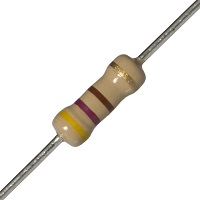
\includegraphics[width=0.05\linewidth]{Componentes/resistencia-470}     \\[0.5cm] \hline
	      2       &         5         & Resistencias 10k Ohm - 1/4W  & R11 R13 R14 R15 R16                 &    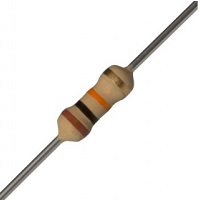
\includegraphics[width=0.05\linewidth]{Componentes/resistencia-10k}     \\[0.5cm] \hline
	      3       &         2         & Capacitores Cerámicos 22pF   & C2 C3                               &     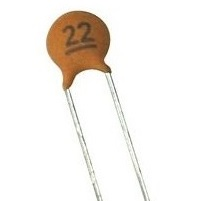
\includegraphics[width=0.05\linewidth]{Componentes/capacitor-22pf}     \\[0.5cm] \hline
	      4       &         5         & Capacitores Cerámicos 0.1uF  & C9 C10 C11 (C12 C13)                &     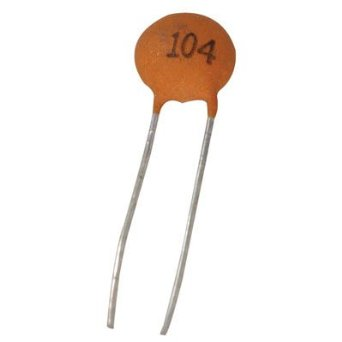
\includegraphics[width=0.05\linewidth]{Componentes/capacitor-01uf}     \\[0.5cm] \hline
	      5       &         1         & Capacitor Cerámico 220nF     & C1                                  &    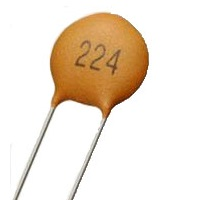
\includegraphics[width=0.05\linewidth]{Componentes/capacitor-220nf}     \\[0.5cm] \hline
	      6       &         1         & Capacitor Electrol. 10uF 16V & C5                                  & 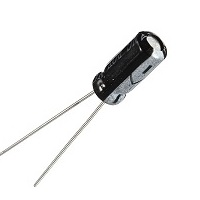
\includegraphics[width=0.05\linewidth]{Componentes/capacitorelectrolitico} \\[0.5cm] \hline
	      7       &         4         & Capacitor Electrol. 100uF    & C4 C6 C7 C8                         &    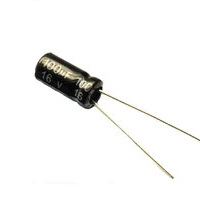
\includegraphics[width=0.05\linewidth]{Componentes/capacitor-100uf}     \\[0.5cm] \hline
	      8       &         3         & Diodos 1N4007                & D9 D12 D14                          &      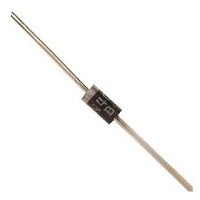
\includegraphics[width=0.05\linewidth]{Componentes/diodo-1n4007}      \\[0.5cm] \hline
	      9       &        11         & Leds difusos 5mm             & D1 D2 D3 D4 D5 D6 D7 D8 D10 D11 D12 &    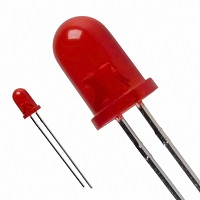
\includegraphics[width=0.05\linewidth]{Componentes/led-difusos-5mm}     \\[0.5cm] \hline
	     10       &         1         & Conector USB hembra Tipo B   & J1                                  &     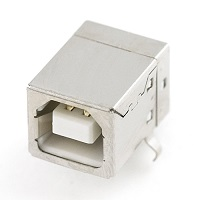
\includegraphics[width=0.05\linewidth]{Componentes/conector-usb-b}     \\[0.4cm] \hline
	     11       &         1         & Push Button (Soft Touch)     & SW2                                 &       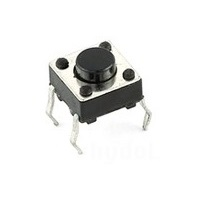
\includegraphics[width=0.05\linewidth]{Componentes/pushbutton}       \\[0.4cm] \hline
\end{tabular} 

\newpage

\begin{tabular}{|c|c|l|p{5cm}|c|}	
	\hline
	\textbf{Item} & \textbf{Cantidad} & \textbf{Componente}                        & \textbf{Ubicación}                           & \textbf{Imagen}                                                                     \\[0.5cm] \hline\hline
	12   & 1        & Regulador de Voltaje LM7805       & U4                                  & 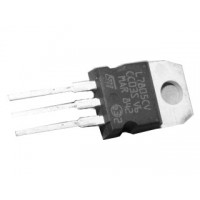
\includegraphics[width=0.05\linewidth]{Componentes/lm7805}                 \\[0.5cm] \hline
	13   & 1        & Regulador de Voltaje 78L05        & U5                                  & 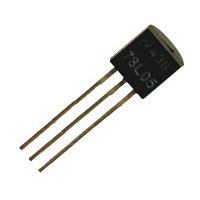
\includegraphics[width=0.05\linewidth]{Componentes/78L05}                  \\[0.5cm] \hline
	14   & 7        & Borneras Dobles                   & P8 P9 P10 P11 P12 P13 P14           & 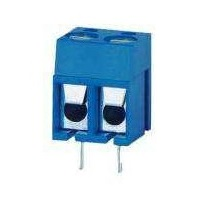
\includegraphics[width=0.05\linewidth]{Componentes/bornera}                \\[0.5cm] \hline
	15   & 1        & Zócalo de 8x2 Pines               & U3                                  & 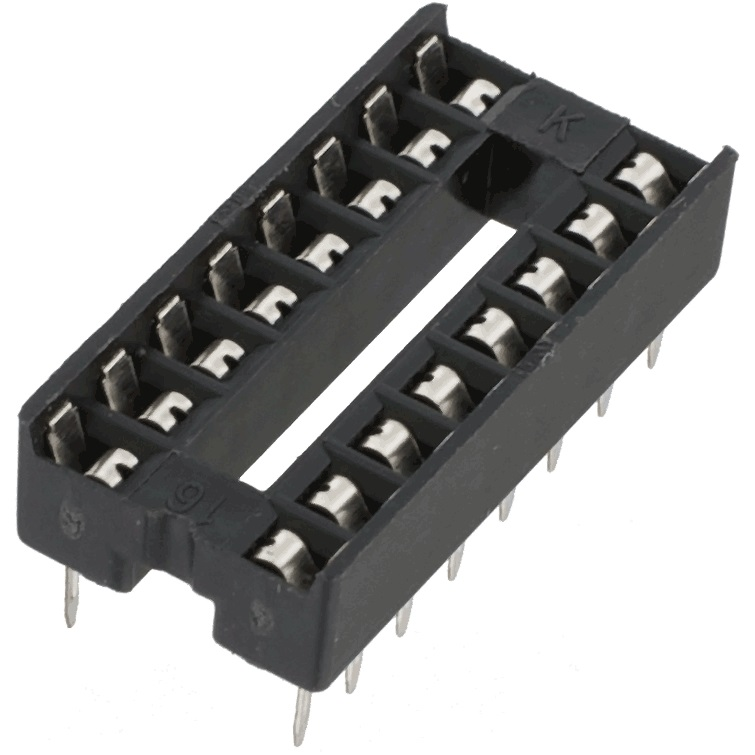
\includegraphics[width=0.05\linewidth]{Componentes/zocalo-8}               \\[0.5cm] \hline
	16   & 1        & Zócalo de 20x2 Pines              & U2                                  & 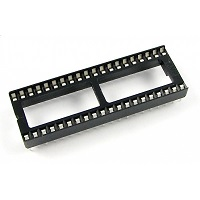
\includegraphics[width=0.05\linewidth]{Componentes/zocalo-20}              \\[0.5cm] \hline
	17   & 1        & Zócalo de 9x2 Pines               & P6                                  & 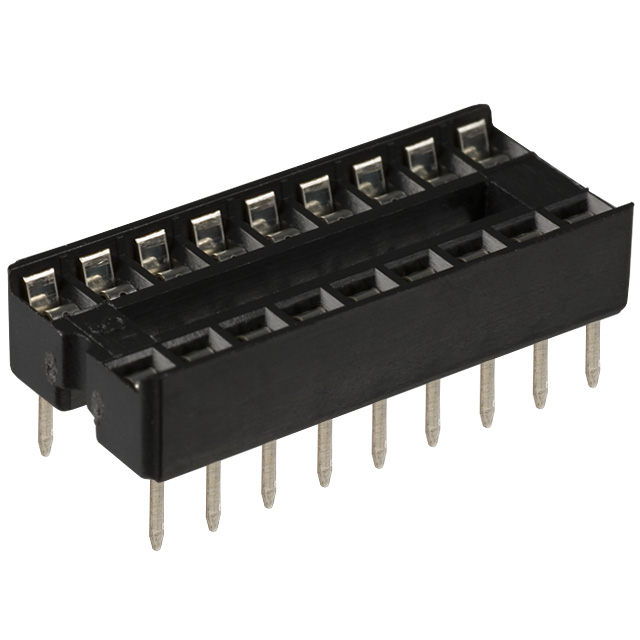
\includegraphics[width=0.05\linewidth]{Componentes/zocalo-9}               \\[0.5cm] \hline
	18   & 1        & Cristal de 20Mhz                  & X1                                  & 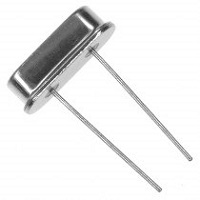
\includegraphics[width=0.05\linewidth]{Componentes/cristal-20mhz}          \\[0.5cm] \hline
	19   & 2        & Tira Postes Macho de 40 Pines     & K2 K3 K4 K5 K6 SW1 SW3 K1 K8 P4     & 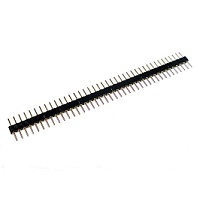
\includegraphics[width=0.05\linewidth]{Componentes/pinesmacho}             \\[0.5cm] \hline
	20   & 1        & Tira de Postes Hembra de 40 Pines & P1 P7 P5 P15 P16 P17 P18            & 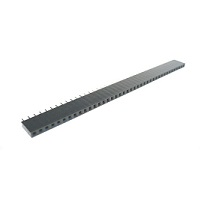
\includegraphics[width=0.05\linewidth]{Componentes/pineshembra}            \\[0.5cm] \hline
	21   & 1        & Driver L293D (Puente H)           & U3                                  & 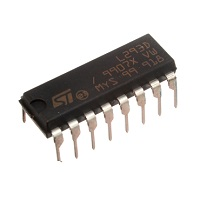
\includegraphics[width=0.05\linewidth]{Componentes/L293D}                  \\[0.5cm] \hline
	22   & 1        & Integrado ULN2803                 & P6                                  & 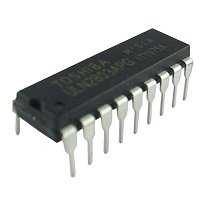
\includegraphics[width=0.05\linewidth]{Componentes/uln2803}                \\[0.5cm] \hline
	23   & 1        & Microcontrolador PIC18F4550       & U2                                  & 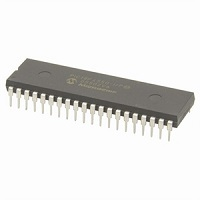
\includegraphics[width=0.05\linewidth]{Componentes/pic18f4550}             \\[0.5cm] \hline
	24   & 1        & Jumper                            & SW1 SW3 K1 K8                       & 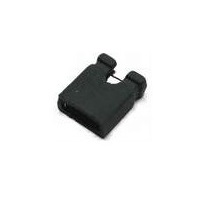
\includegraphics[width=0.05\linewidth]{Componentes/Jumper}                 \\[0.5cm] \hline
\end{tabular} 	
	

\chapter{Herramientas}

Las herramientas que necesitamos para armar una placa robotica np07 son faciles de conseguir y muy comunes para cualquier hobbista de la electronica.

\section{Soldador}

Un soldador eléctrico o de estaño, también conocido como cautín, es una herramienta eléctrica usada para soldar.
Funciona convirtiendo la energía eléctrica en calor, que a su vez provoca la fusión del material utilizado en la soldadura, como por ejemplo el estaño.

\begin{figure}[h]
	\centering
	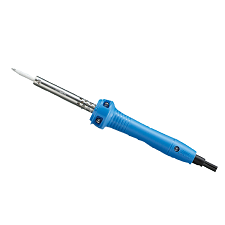
\includegraphics[width=0.5\linewidth]{herramientas/soldador}
	\caption{Soldador}
	\label{fig:soldador}
\end{figure}

\newpage

\section{Estaño}

El estaño que se utiliza en electrónica tiene alma de resina con el fin de facilitar la soldadura. 
Para garantizar una buena soldadura es necesario que tanto el estaño como el elemento a soldar alcancen una temperatura determinada, si esta temperatura no se alcanza se produce el fenómeno denominado soldadura fría. La temperatura de fusión depende de la aleación utilizada, cuyo componente principal es el estaño y suele estar comprendida entre unos 200 a 400 grados celsius.
En realidad, el término “estaño” se emplea de forma impropia porque no se trata de estaño sólo, sino de una aleación de este metal con plomo, generalmente con una proporción respectiva del 60 y del 40 por ciento, que resulta ser la más indicada para las soldaduras en Electrónica. 
Para realizar una buena soldadura, además del soldador y de la aleación descrita, se necesita una sustancia adicional, llamada pasta de soldar, cuya misión es la de facilitar la distribución uniforme del estaño sobre las super?cies a unir y evitando, al mismo tiempo, la oxidación producida por la temperatura demasiado elevada del soldador.
La composición de esta pasta es a base de colofonia (normalmente llamada “resina”) y que en el caso del estaño que utilizaremos, está contenida dentro de las cavidades del hilo, en una proporción del 2 a 2.5 por ciento.

\begin{figure}[h]
	\centering
	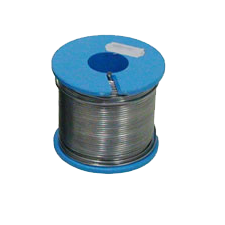
\includegraphics[width=0.5\linewidth]{herramientas/estanio}
	\caption{Estaño}
	\label{fig:estanio}
\end{figure}

\newpage

\section{Pinza}

Un pequeño alicate, para poder cortar el excedente de material (estaño, alambres de las resistensias por ejmplo).

\begin{figure}[h]
	\centering
	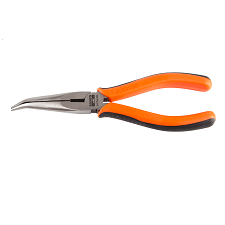
\includegraphics[width=0.5\linewidth]{herramientas/pinza}
	\caption{Alicate para Electronica}
	\label{fig:pinza}
\end{figure}

\newpage

\section{Destornillador}

Nos sirve para ajustar las borneras y para hacer palanca para sacar un integrado que hayamos puesto en un zocalo.

\begin{figure}[h]
	\centering
	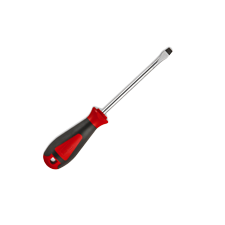
\includegraphics[width=0.5\linewidth]{herramientas/destornillador}
	\caption{Destornillador Plano Pequeño}
	\label{fig:destornillador}
\end{figure}

\newpage

\section{Desoldador de Estaño}

El desoldador de estaño, nos permite sacar el estaño que hayamos puesto de mas o para remplazar algun componente efectuoso de la placa robotica np07

\begin{figure}[h]
	\centering
	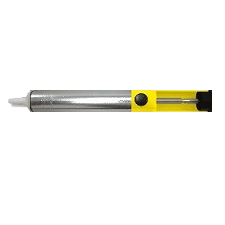
\includegraphics[width=0.5\linewidth]{herramientas/desoldador}
	\caption{Desoldador de Estaño}
	\label{fig:desoldador}
\end{figure}



\chapter{Fabricación}

A continución veremos el paso a paso del armado de la placa np07.
\\

Lo vamos a dividir en 6 Módulos:


\begin{enumerate}
	
	\item Módulo 1: Preparación
	\item Módulo 2: Microcontrolador
	\item Módulo 3: Leds y sensores digitales
	\item Módulo 4: Sensores analógicos y servos
	\item Módulo 5: Motores de Corriente Continua
	\item Módulo 6: Fuente de poder externa

\end{enumerate}



\chapter{Módulo 1: Preparación}

Iniciaremos con la placa np07

\begin{figure}[h]
	\centering
	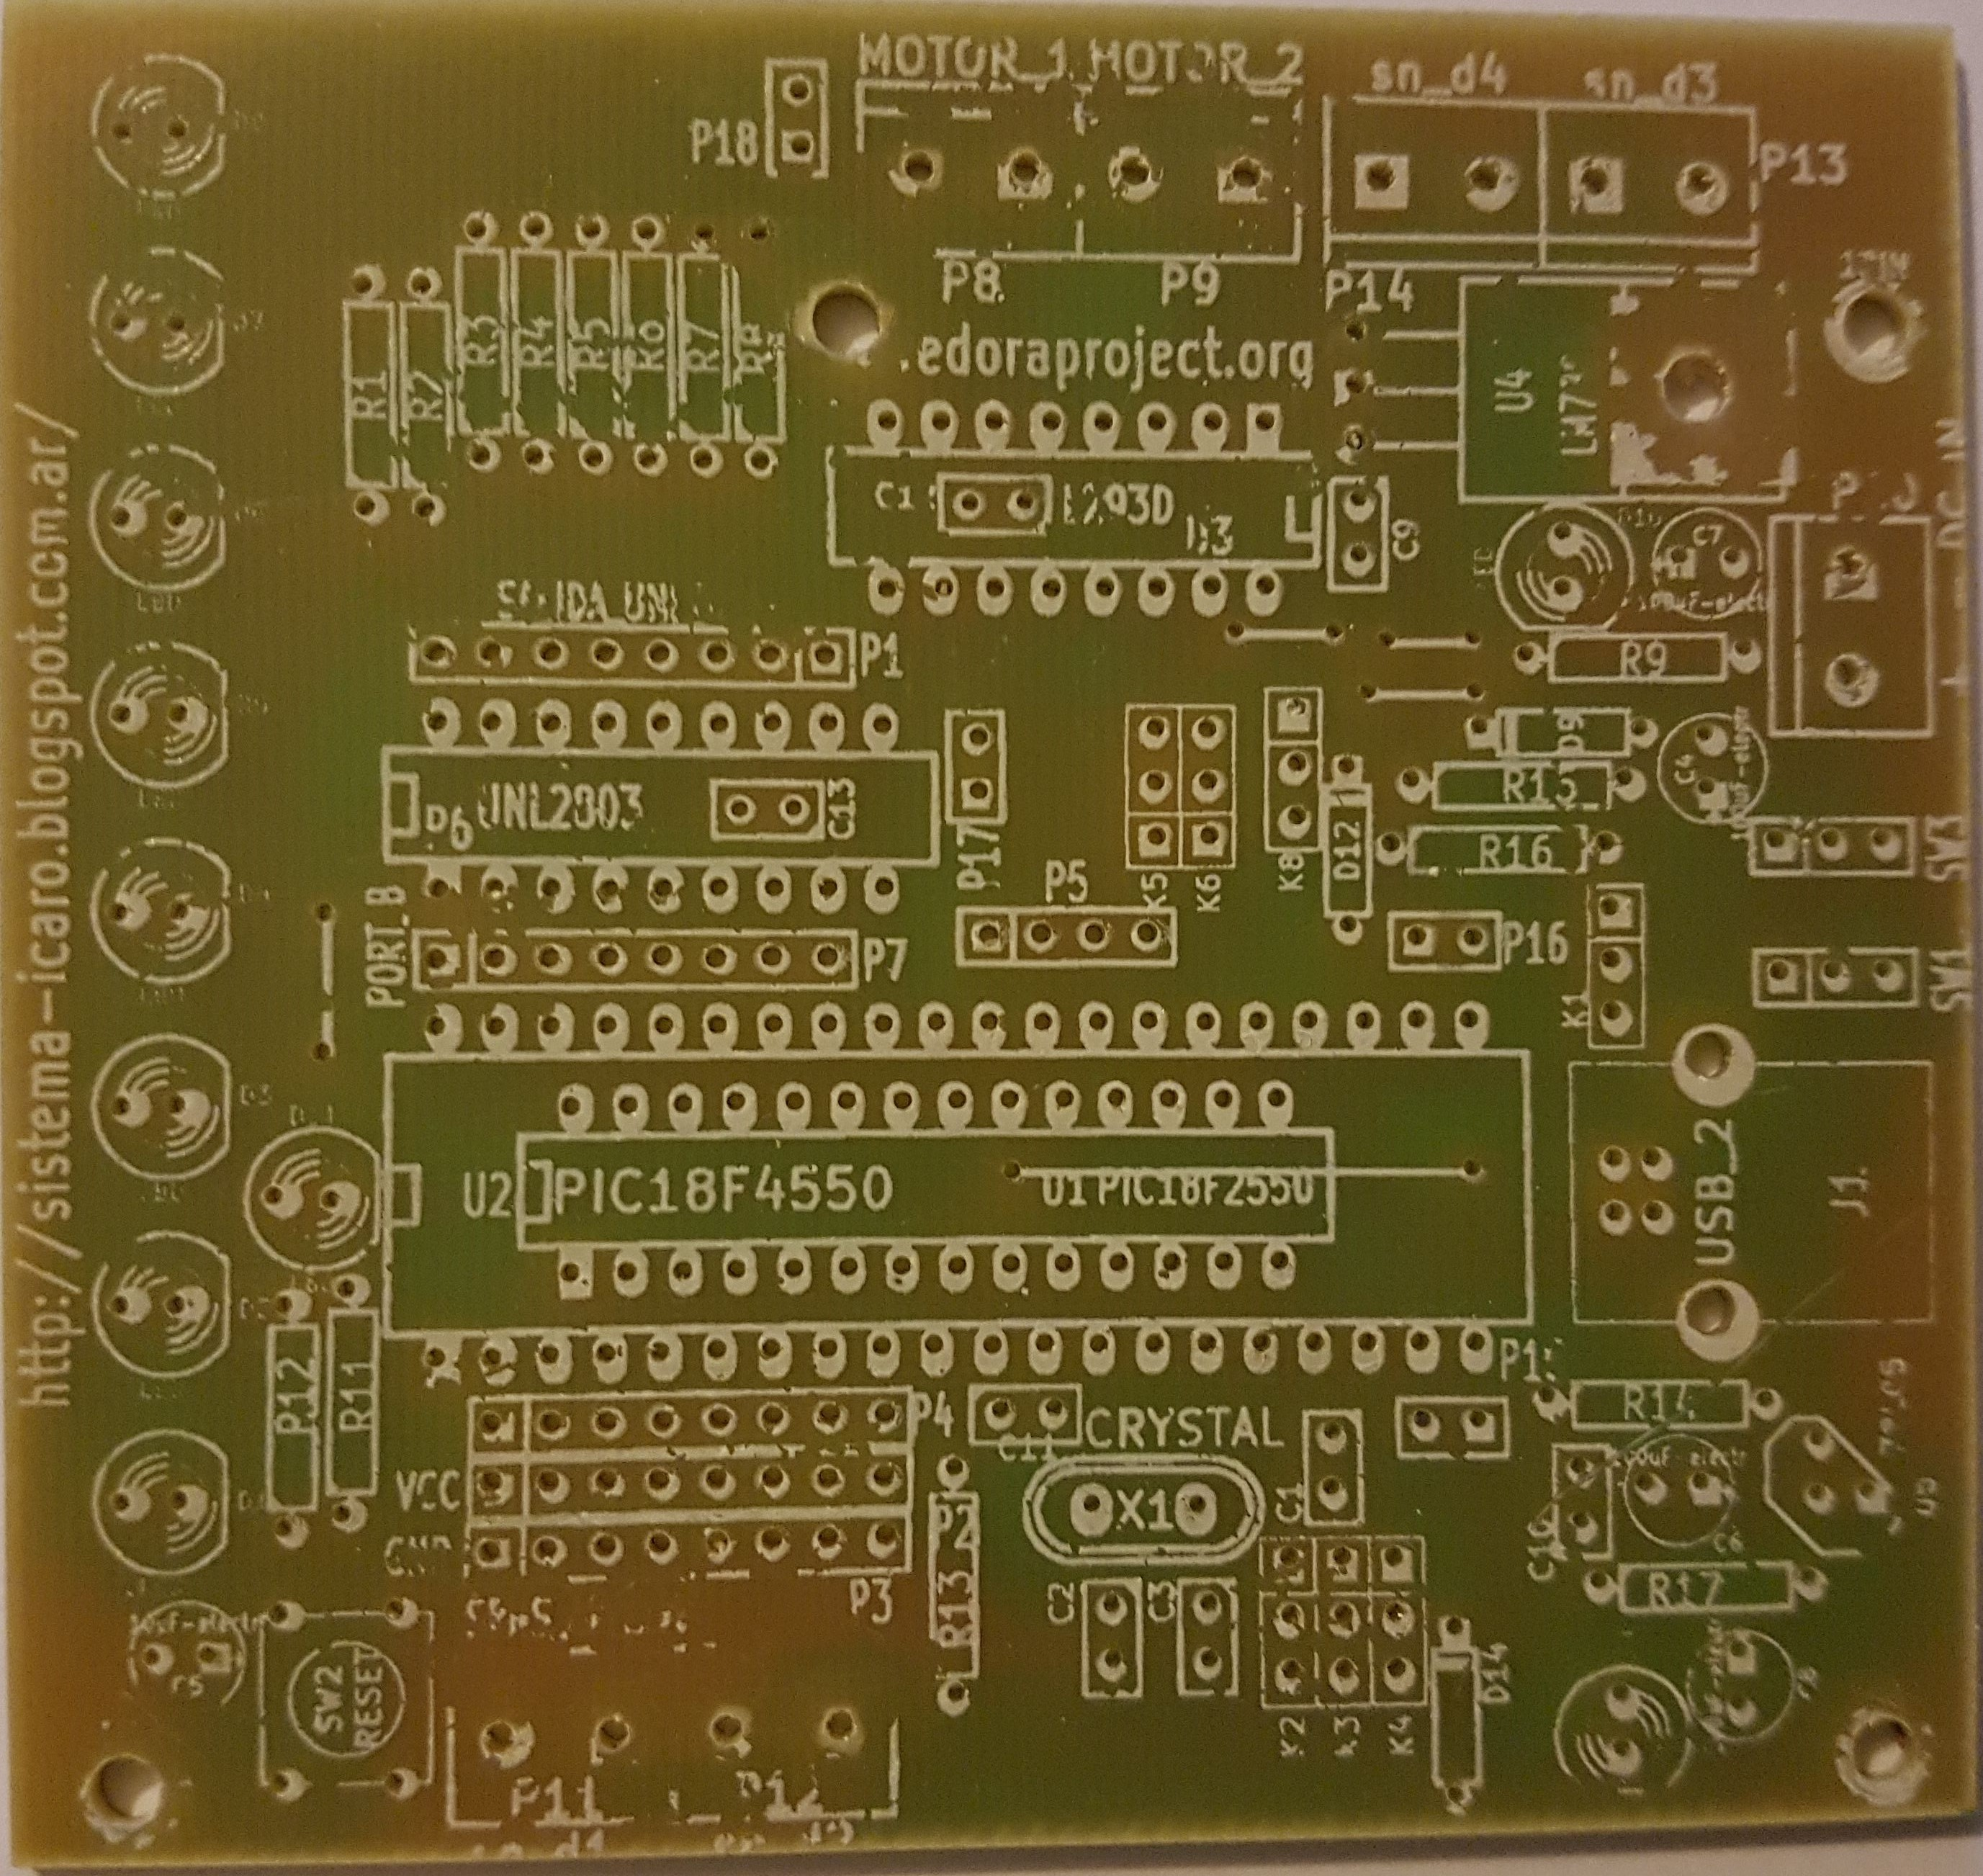
\includegraphics[width=0.8\linewidth]{Modulo_1/M1_0}
	\caption{Módulo 1 - Placa np07}
	\label{fig:M1_0}
\end{figure}

\newpage

\section{Paso 1:}

Instalar los 5 puentes de la placa. Para el puente que quedará bajo el Microcontrolador se requiere un pedazo de cable. Lo más común es cable UTP de redes, pelado. La cubierta del cable se derretirá de todas formas al soldarlo. Los otros puentes se pueden hacer usando más de este tipo de cable o se puede usar patitas de resistencias.

\begin{figure}[h]
	\centering
	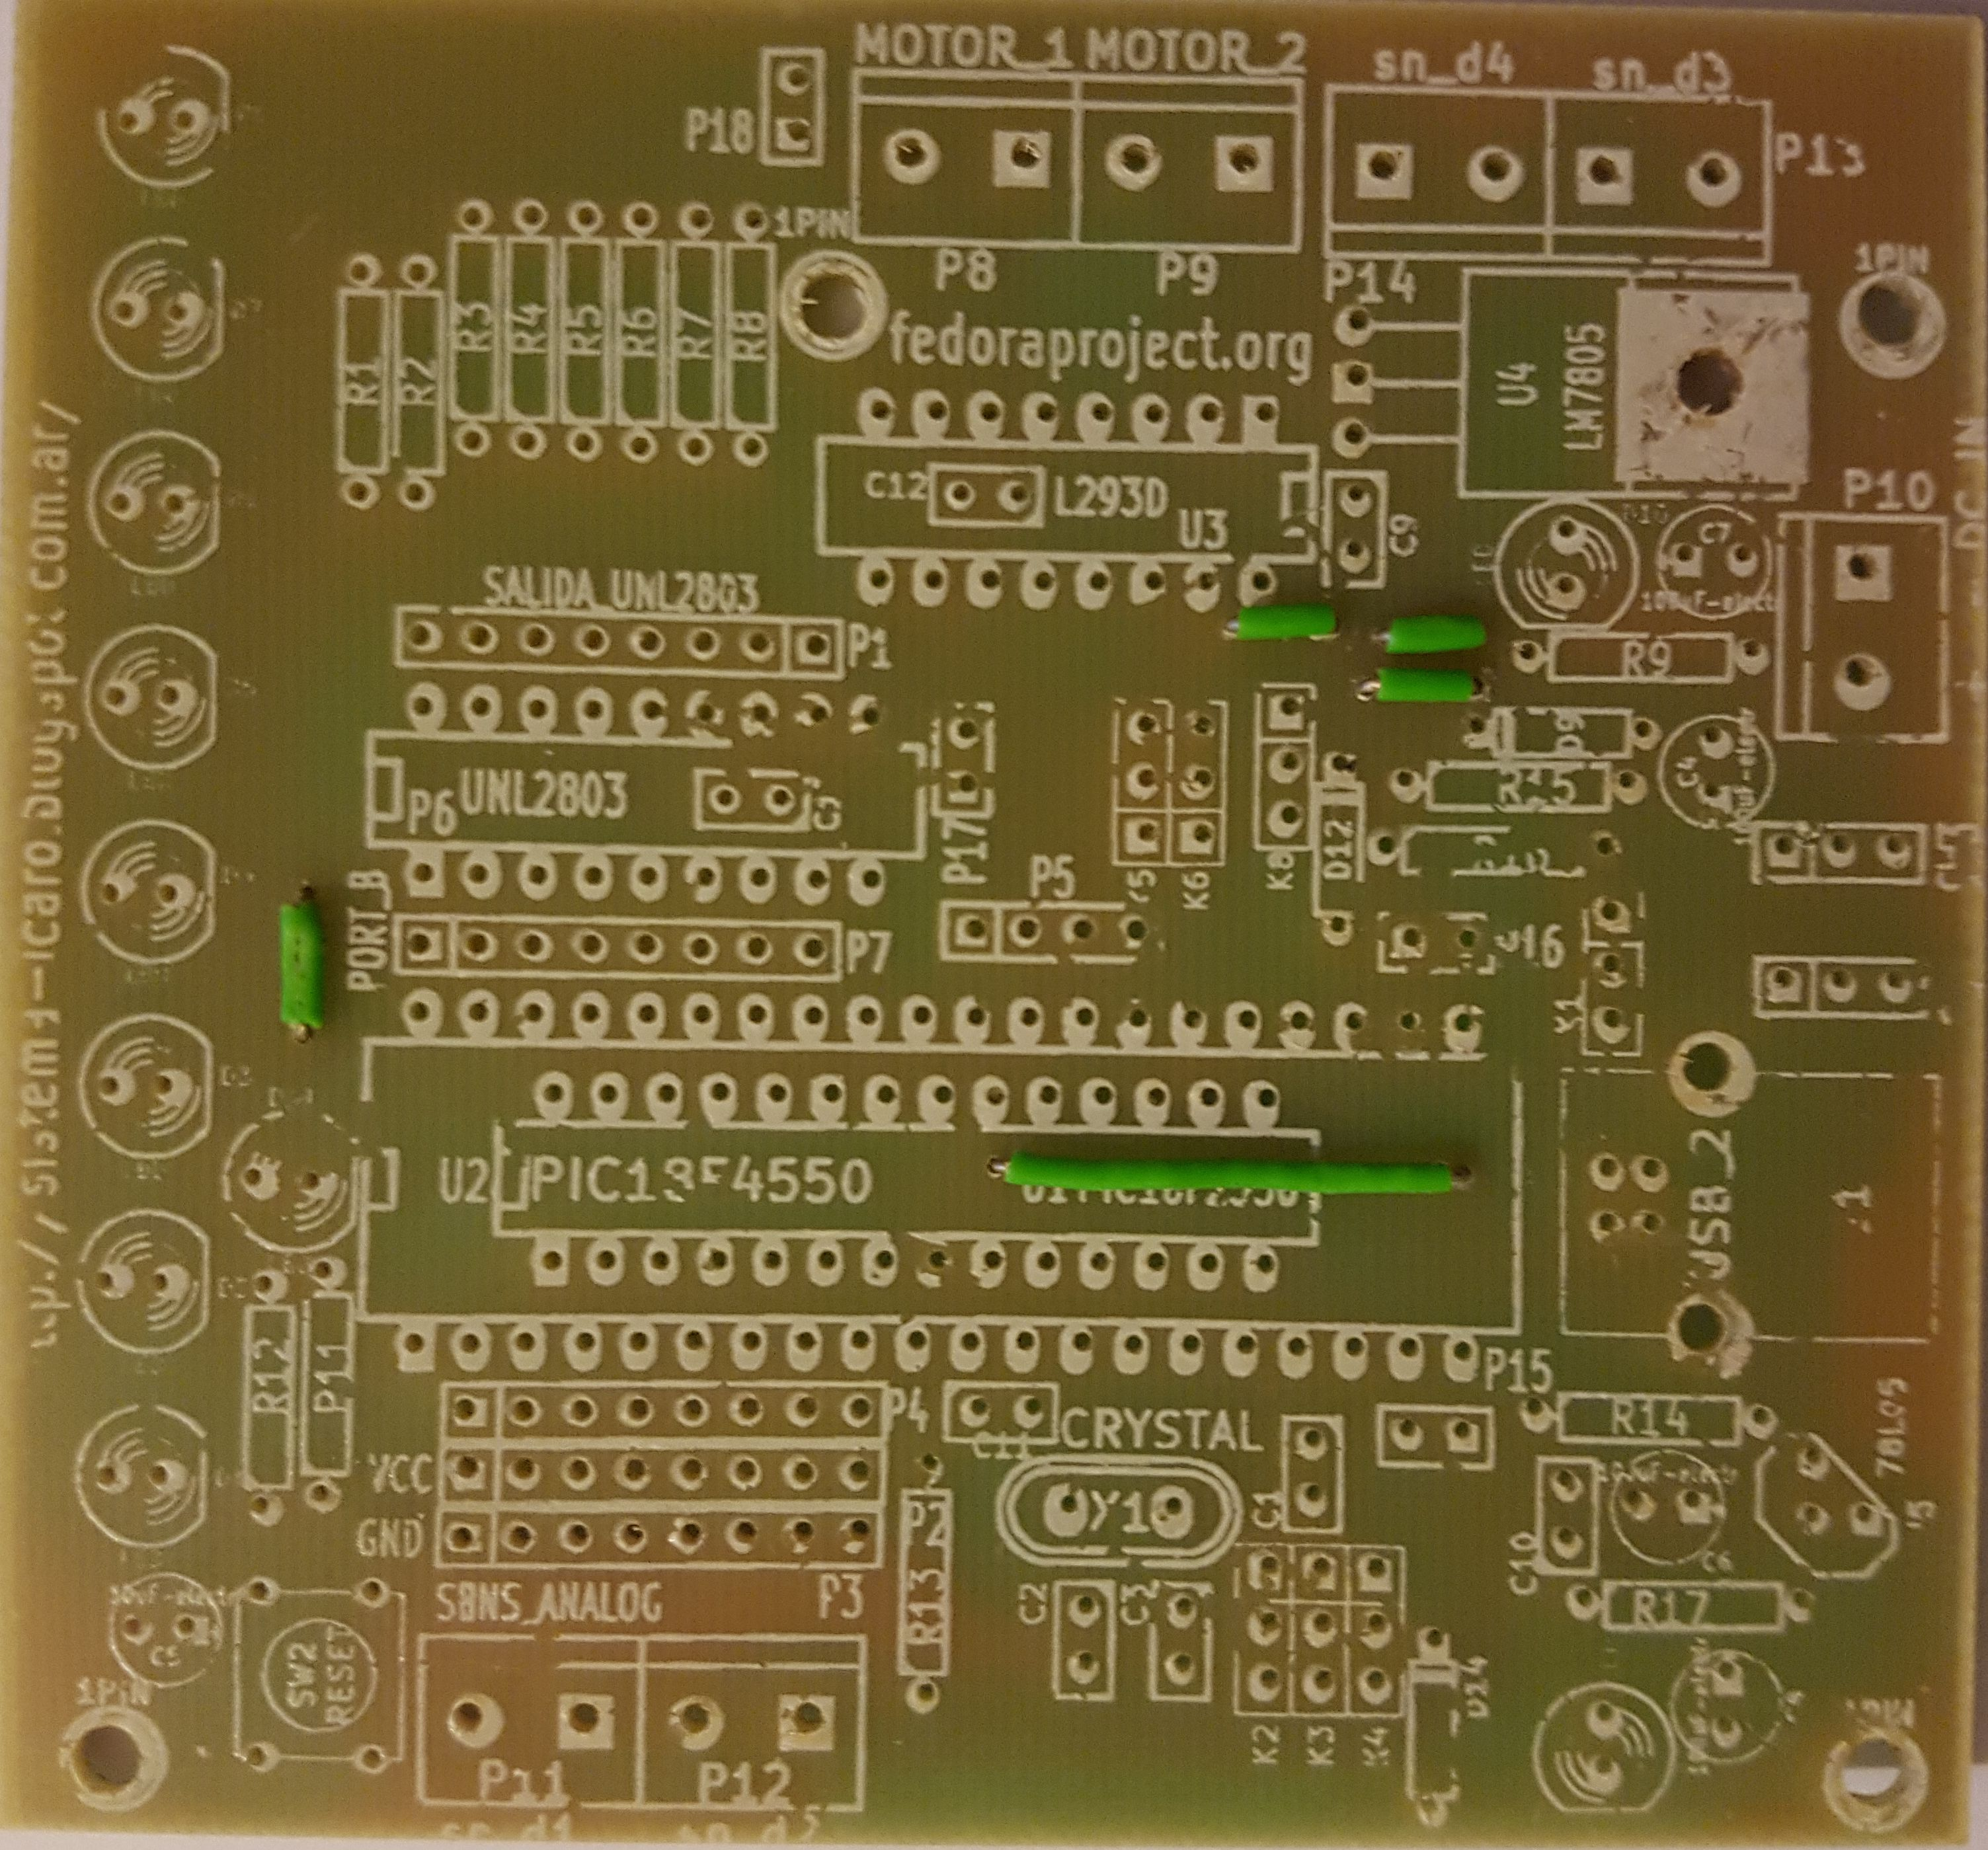
\includegraphics[width=0.8\linewidth]{Modulo_1/M1_1}
	\caption{Módulo 1 - Paso 1}
	\label{fig:M1_1}
\end{figure}

\newpage

\section{Paso 2:}

Instalar todos los diodos. D9, D12 y D14

\begin{figure}[h]
	\centering
	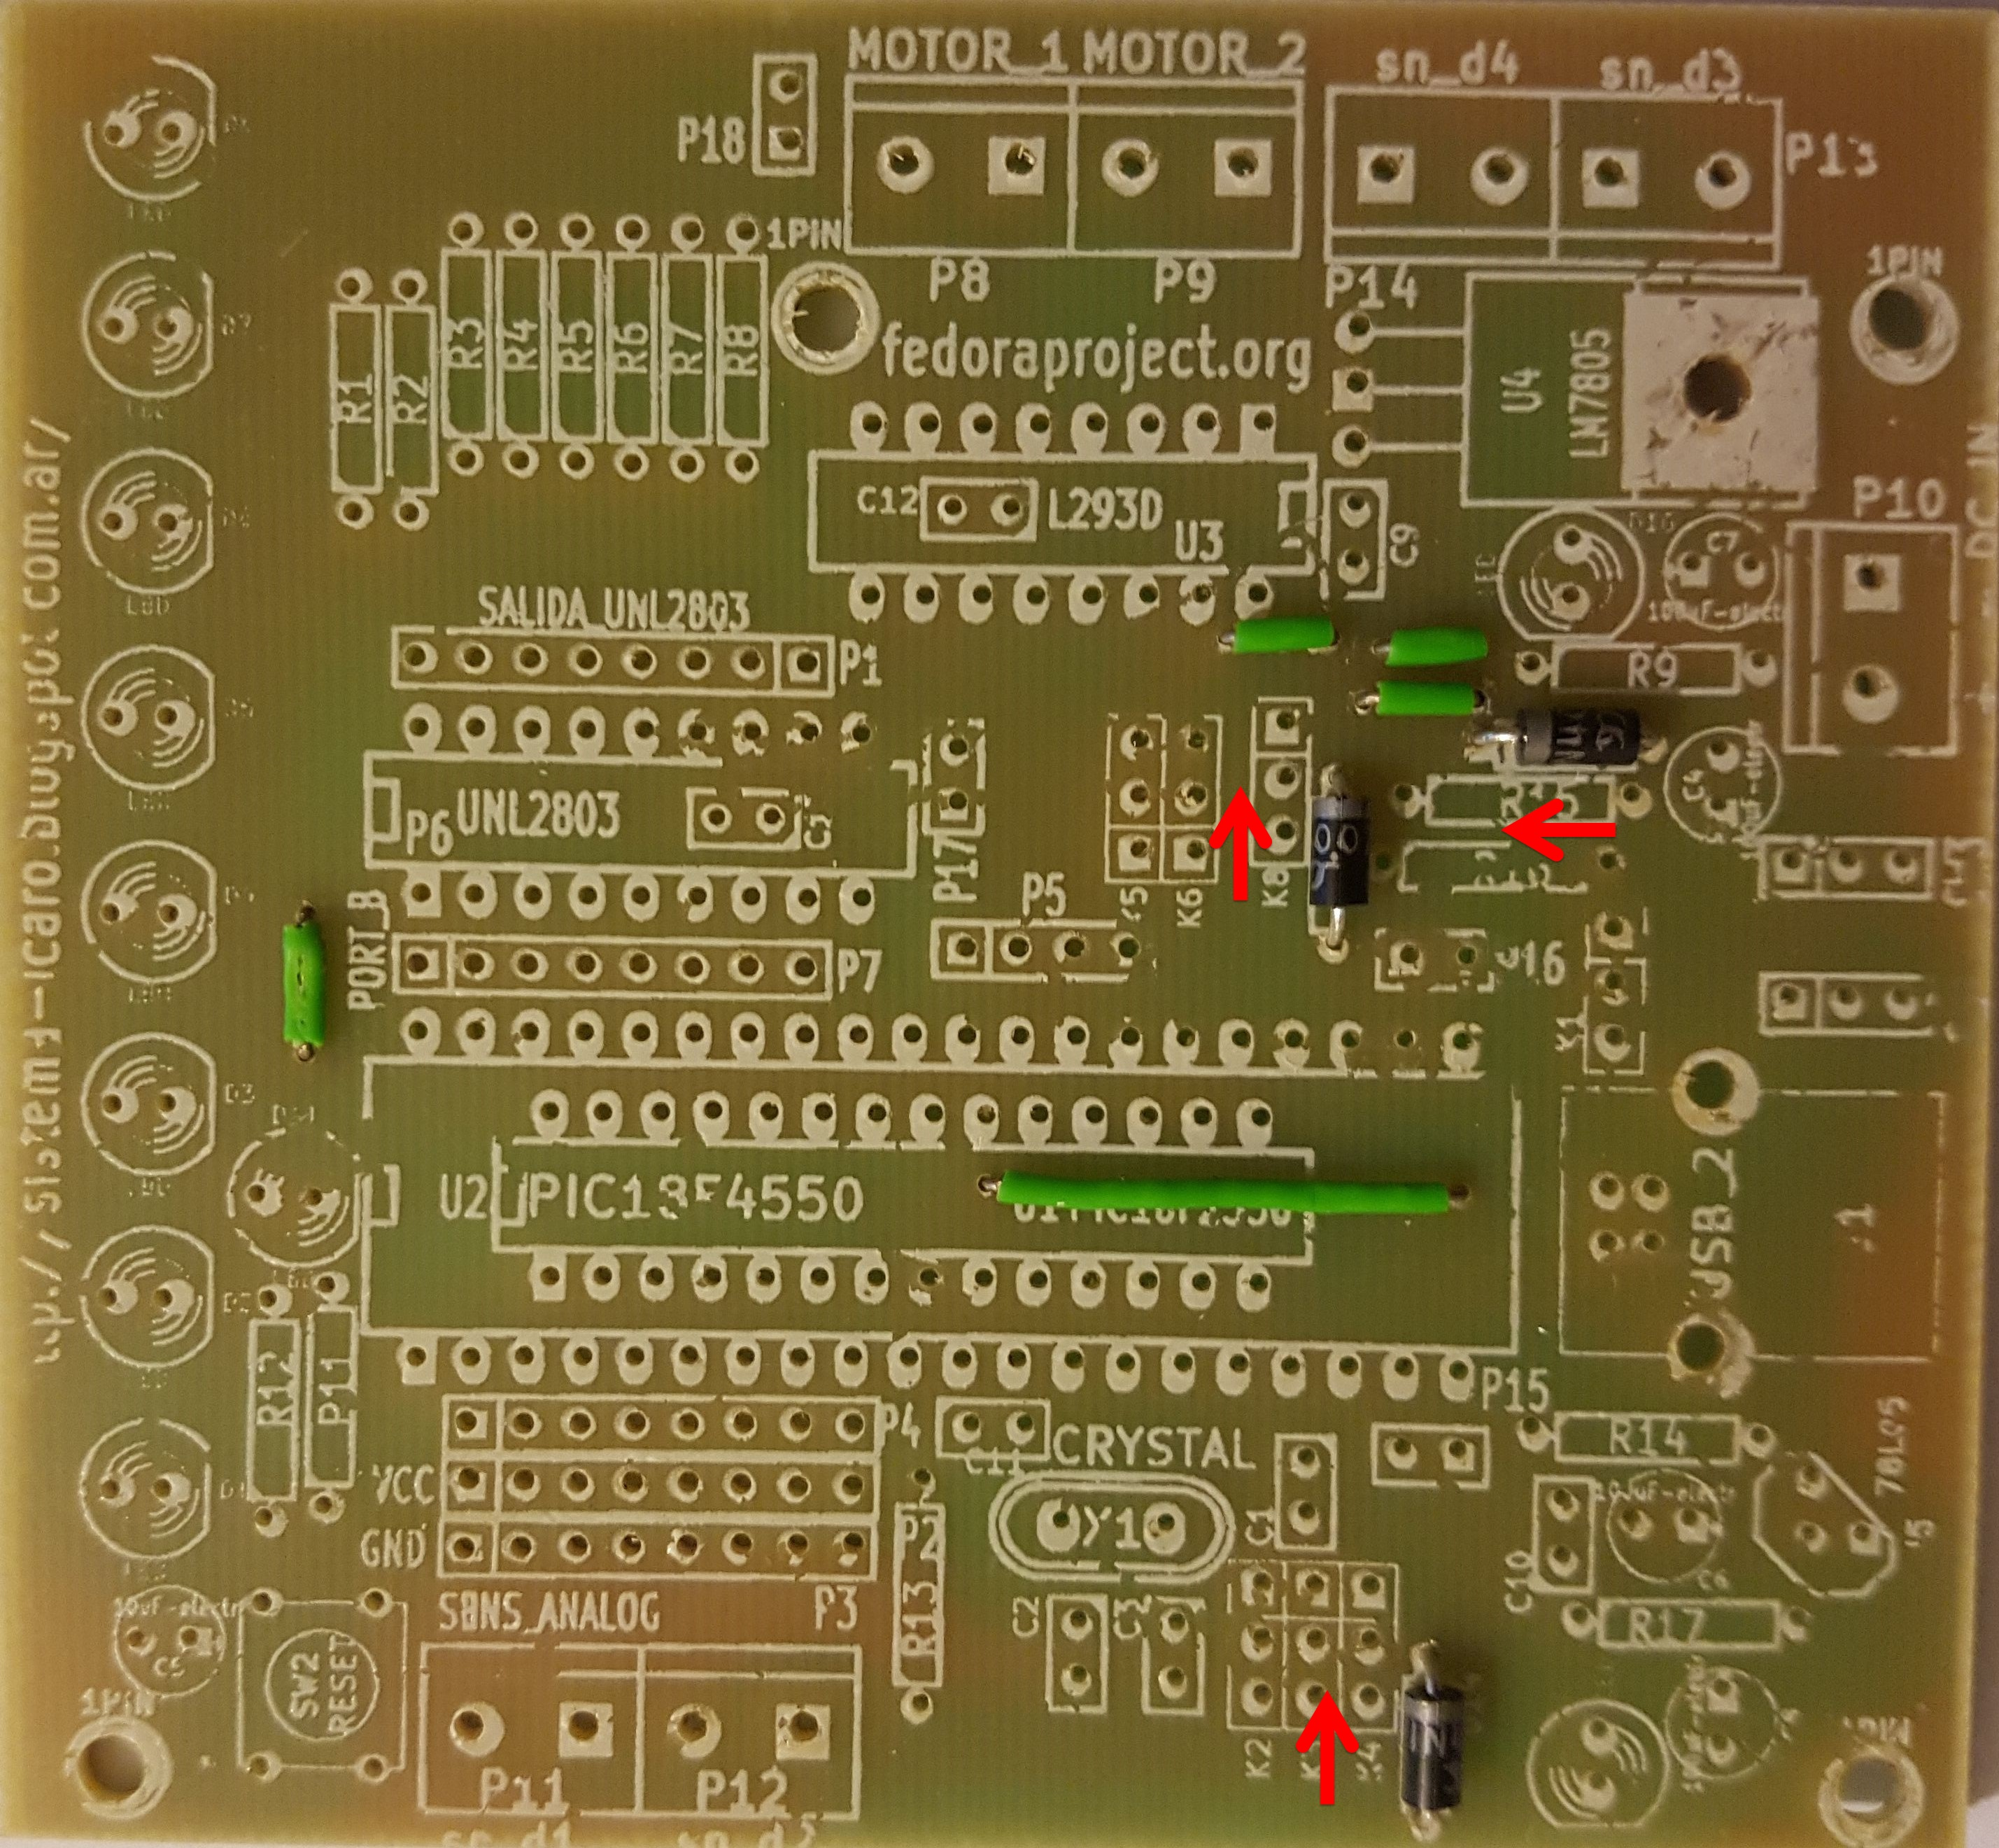
\includegraphics[width=0.8\linewidth]{Modulo_1/M1_2}
	\caption{Módulo 1 - Paso 2}
	\label{fig:M1_2}
\end{figure}

\newpage

\section{Paso 3:}

Instalar las resistencias de 470 Ohm. R9, R12 y R17

\begin{figure}[h]
	\centering
	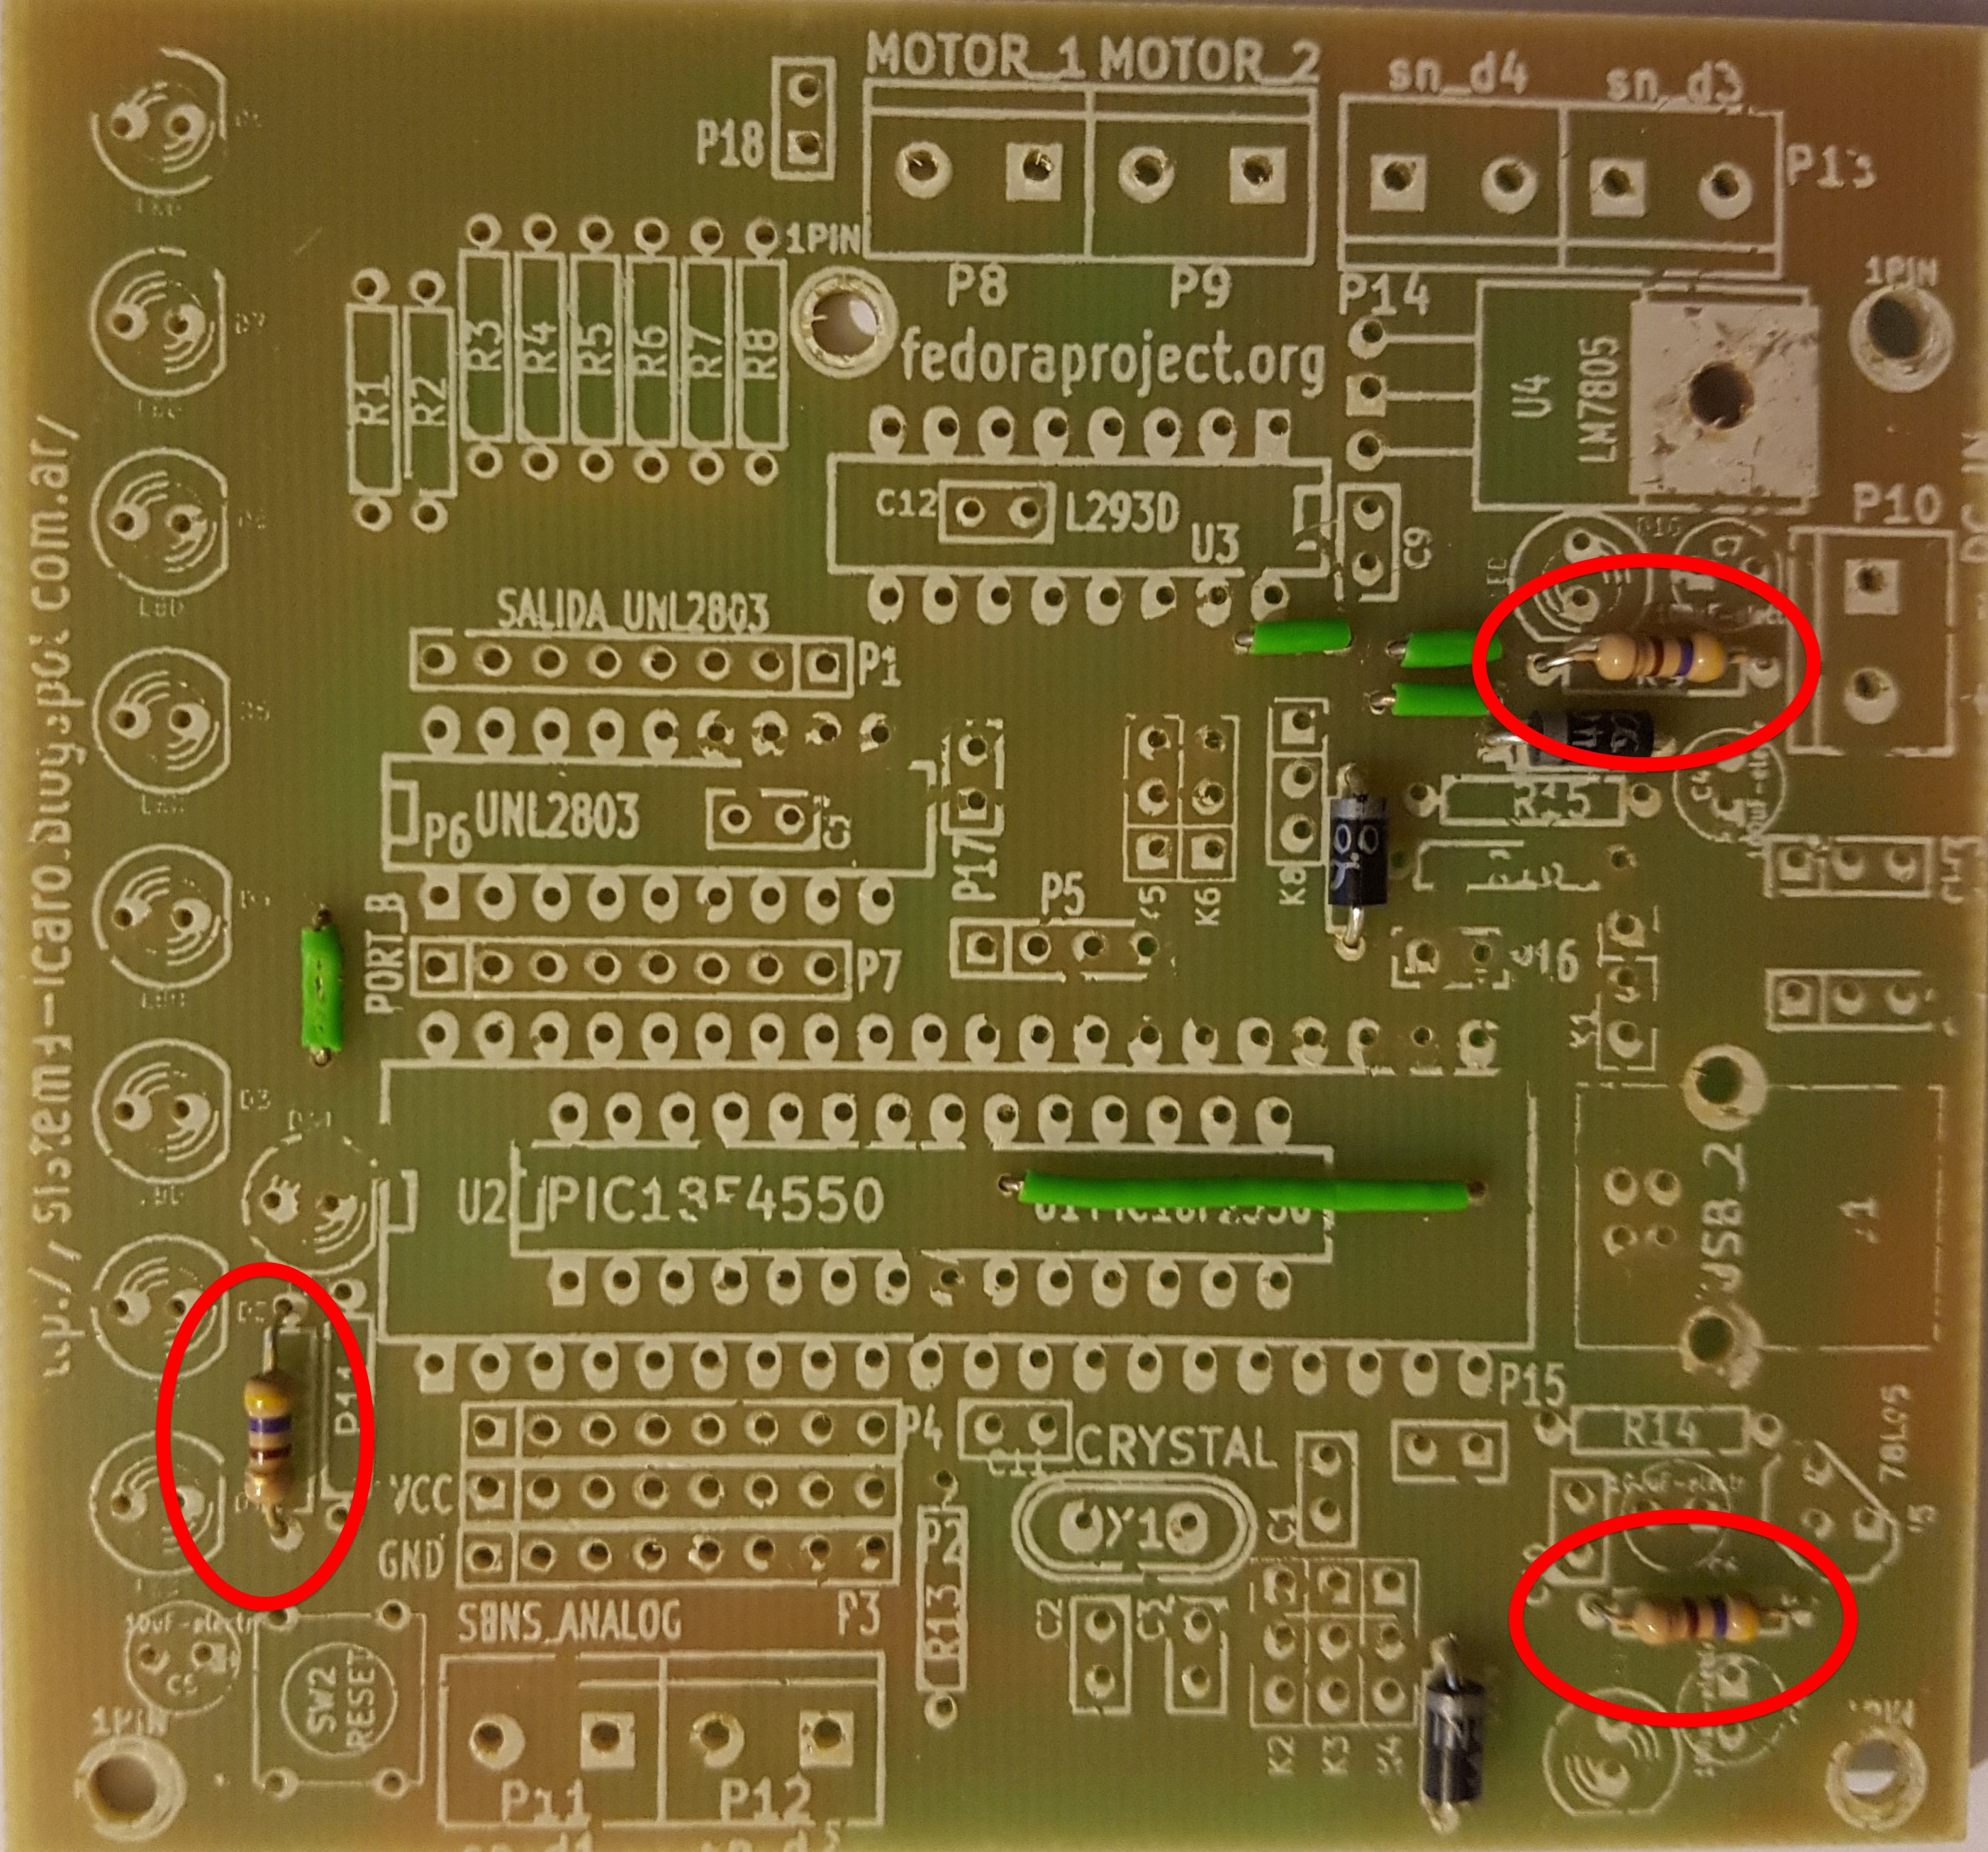
\includegraphics[width=0.8\linewidth]{Modulo_1/M1_3}
	\caption{Módulo 1 - Paso 3}
	\label{fig:M1_3}
\end{figure}

\newpage

\section{Paso 4:}

Instalar las resistencias de 10K Ohm. R11, R13, R14, R15 y R16

\begin{figure}[h]
	\centering
	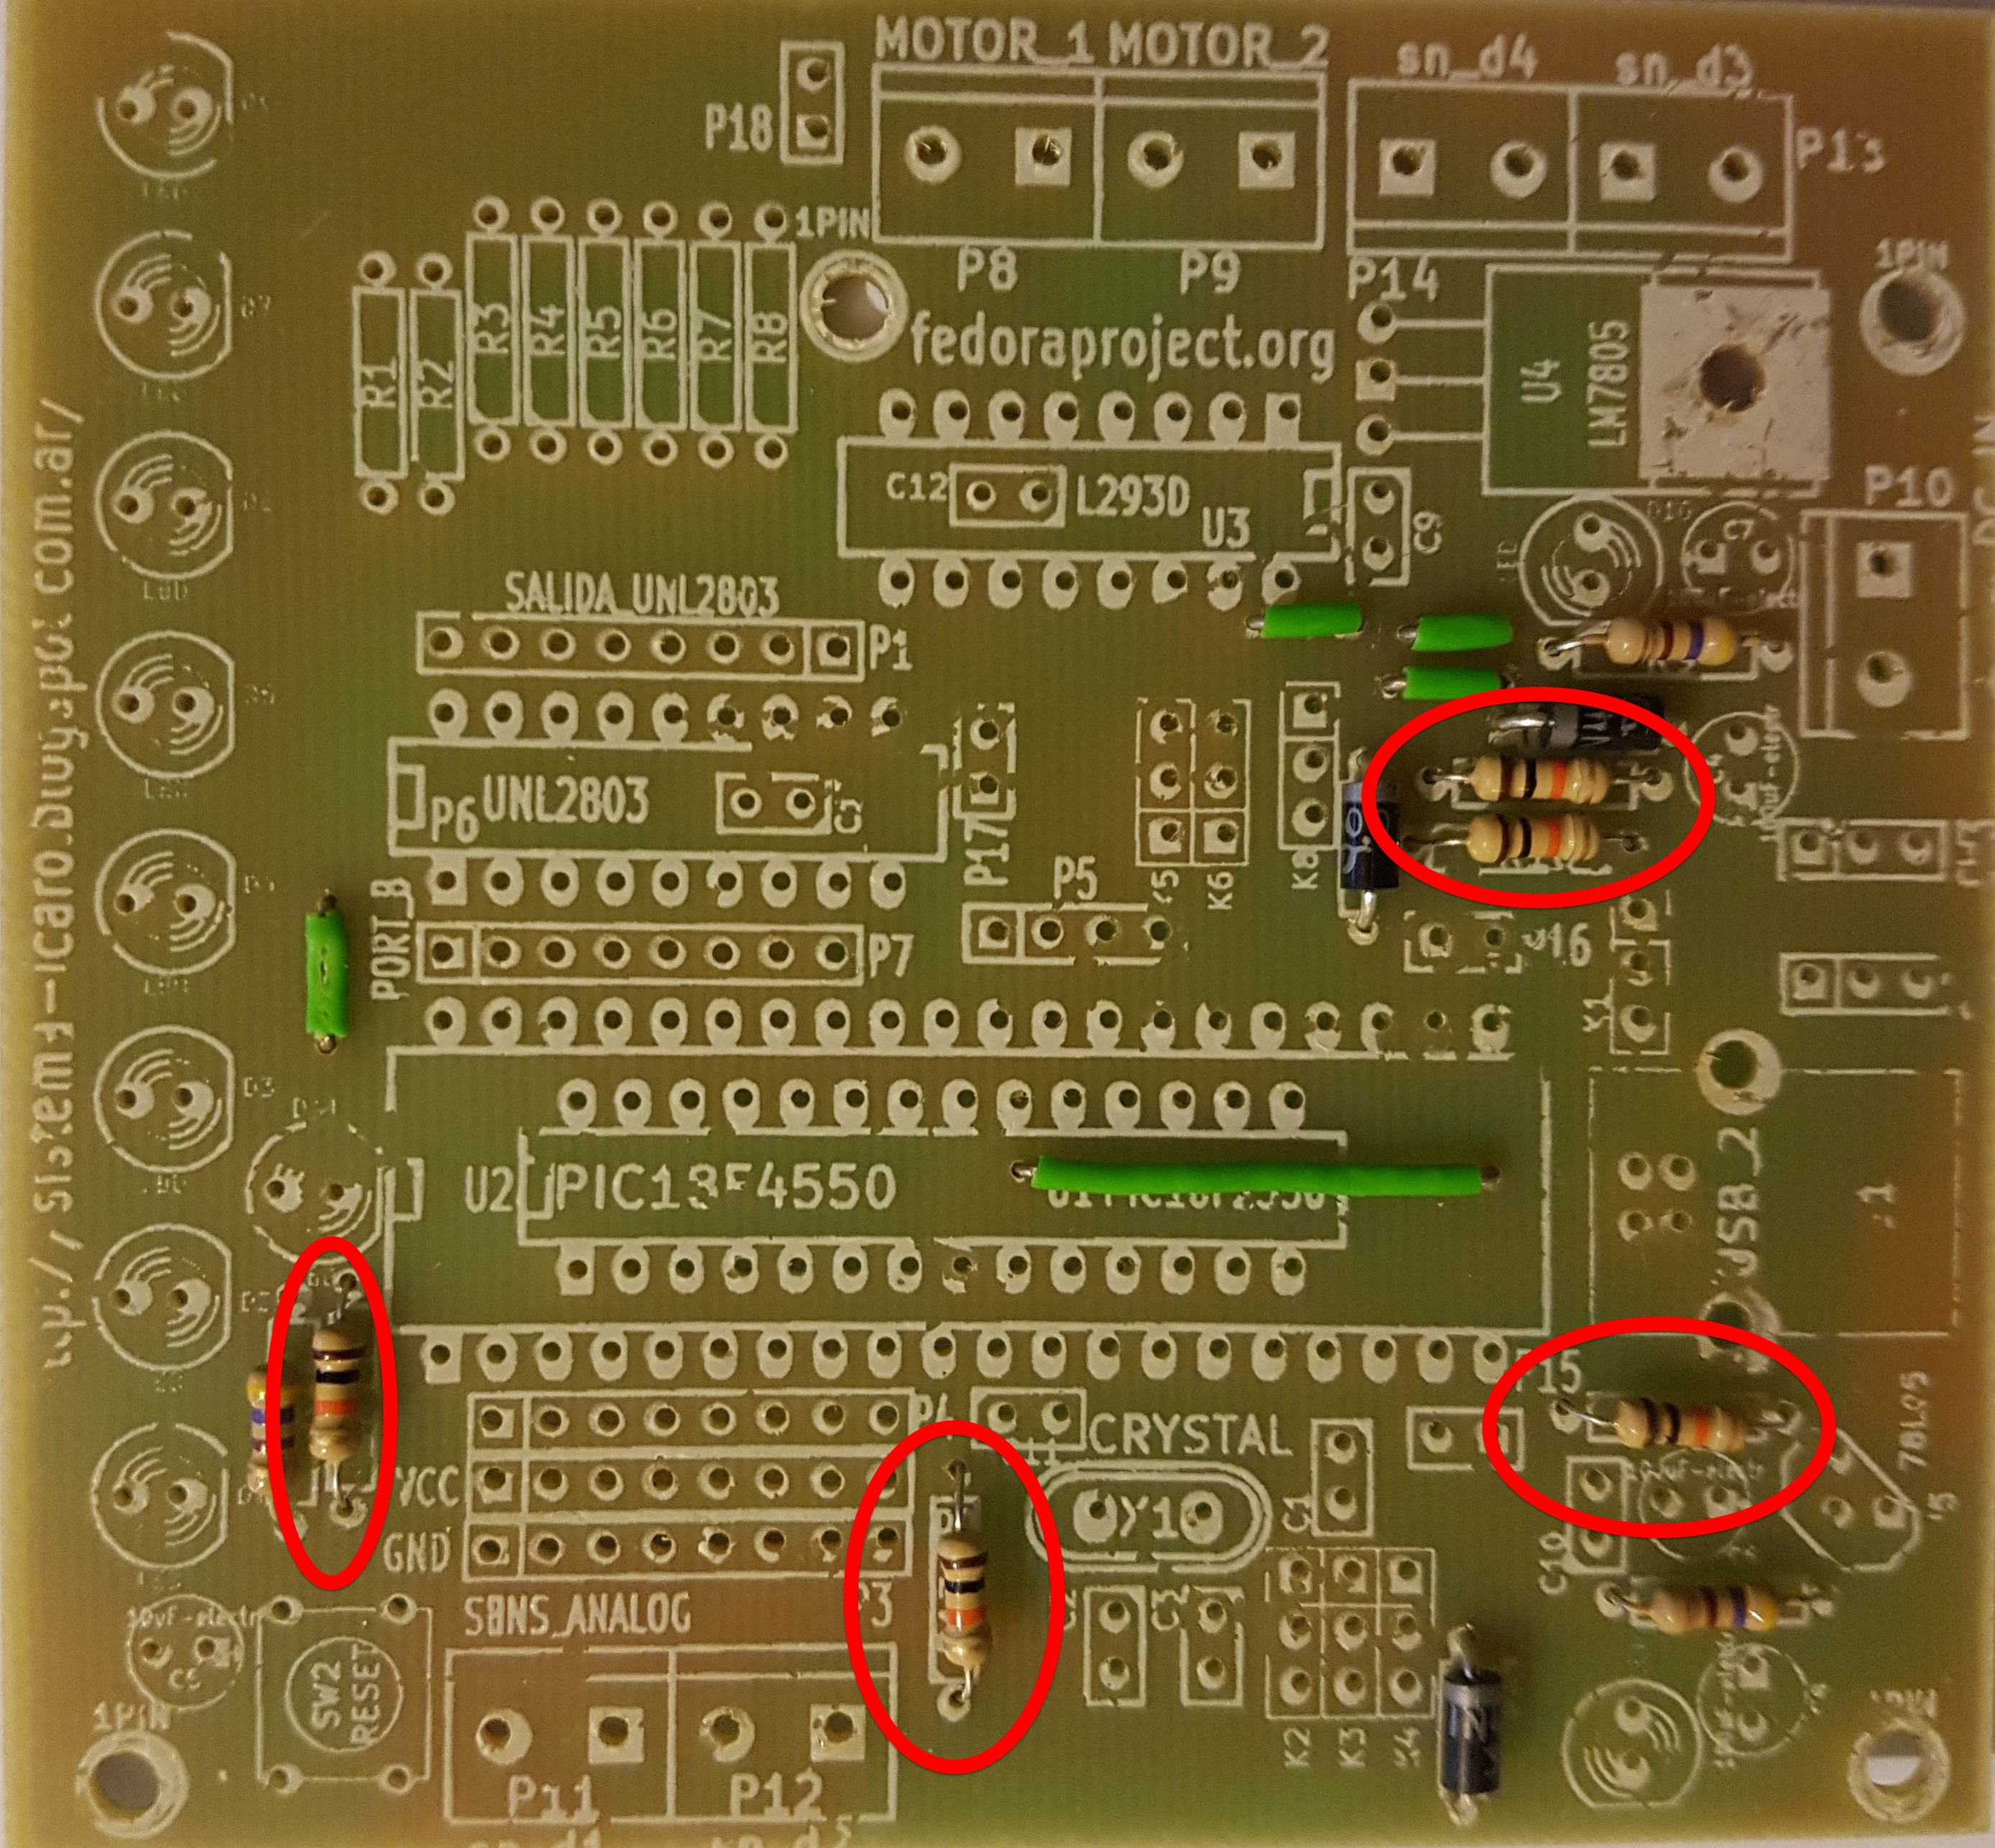
\includegraphics[width=0.8\linewidth]{Modulo_1/M1_4}
	\caption{Módulo 1 - Paso 4}
	\label{fig:M1_4}
\end{figure}



\chapter{Módulo 2: Microcontrolador}

\section{Paso 1:}

Instalar cristal de 20Mhz. X1

\begin{figure}[h]
	\centering
	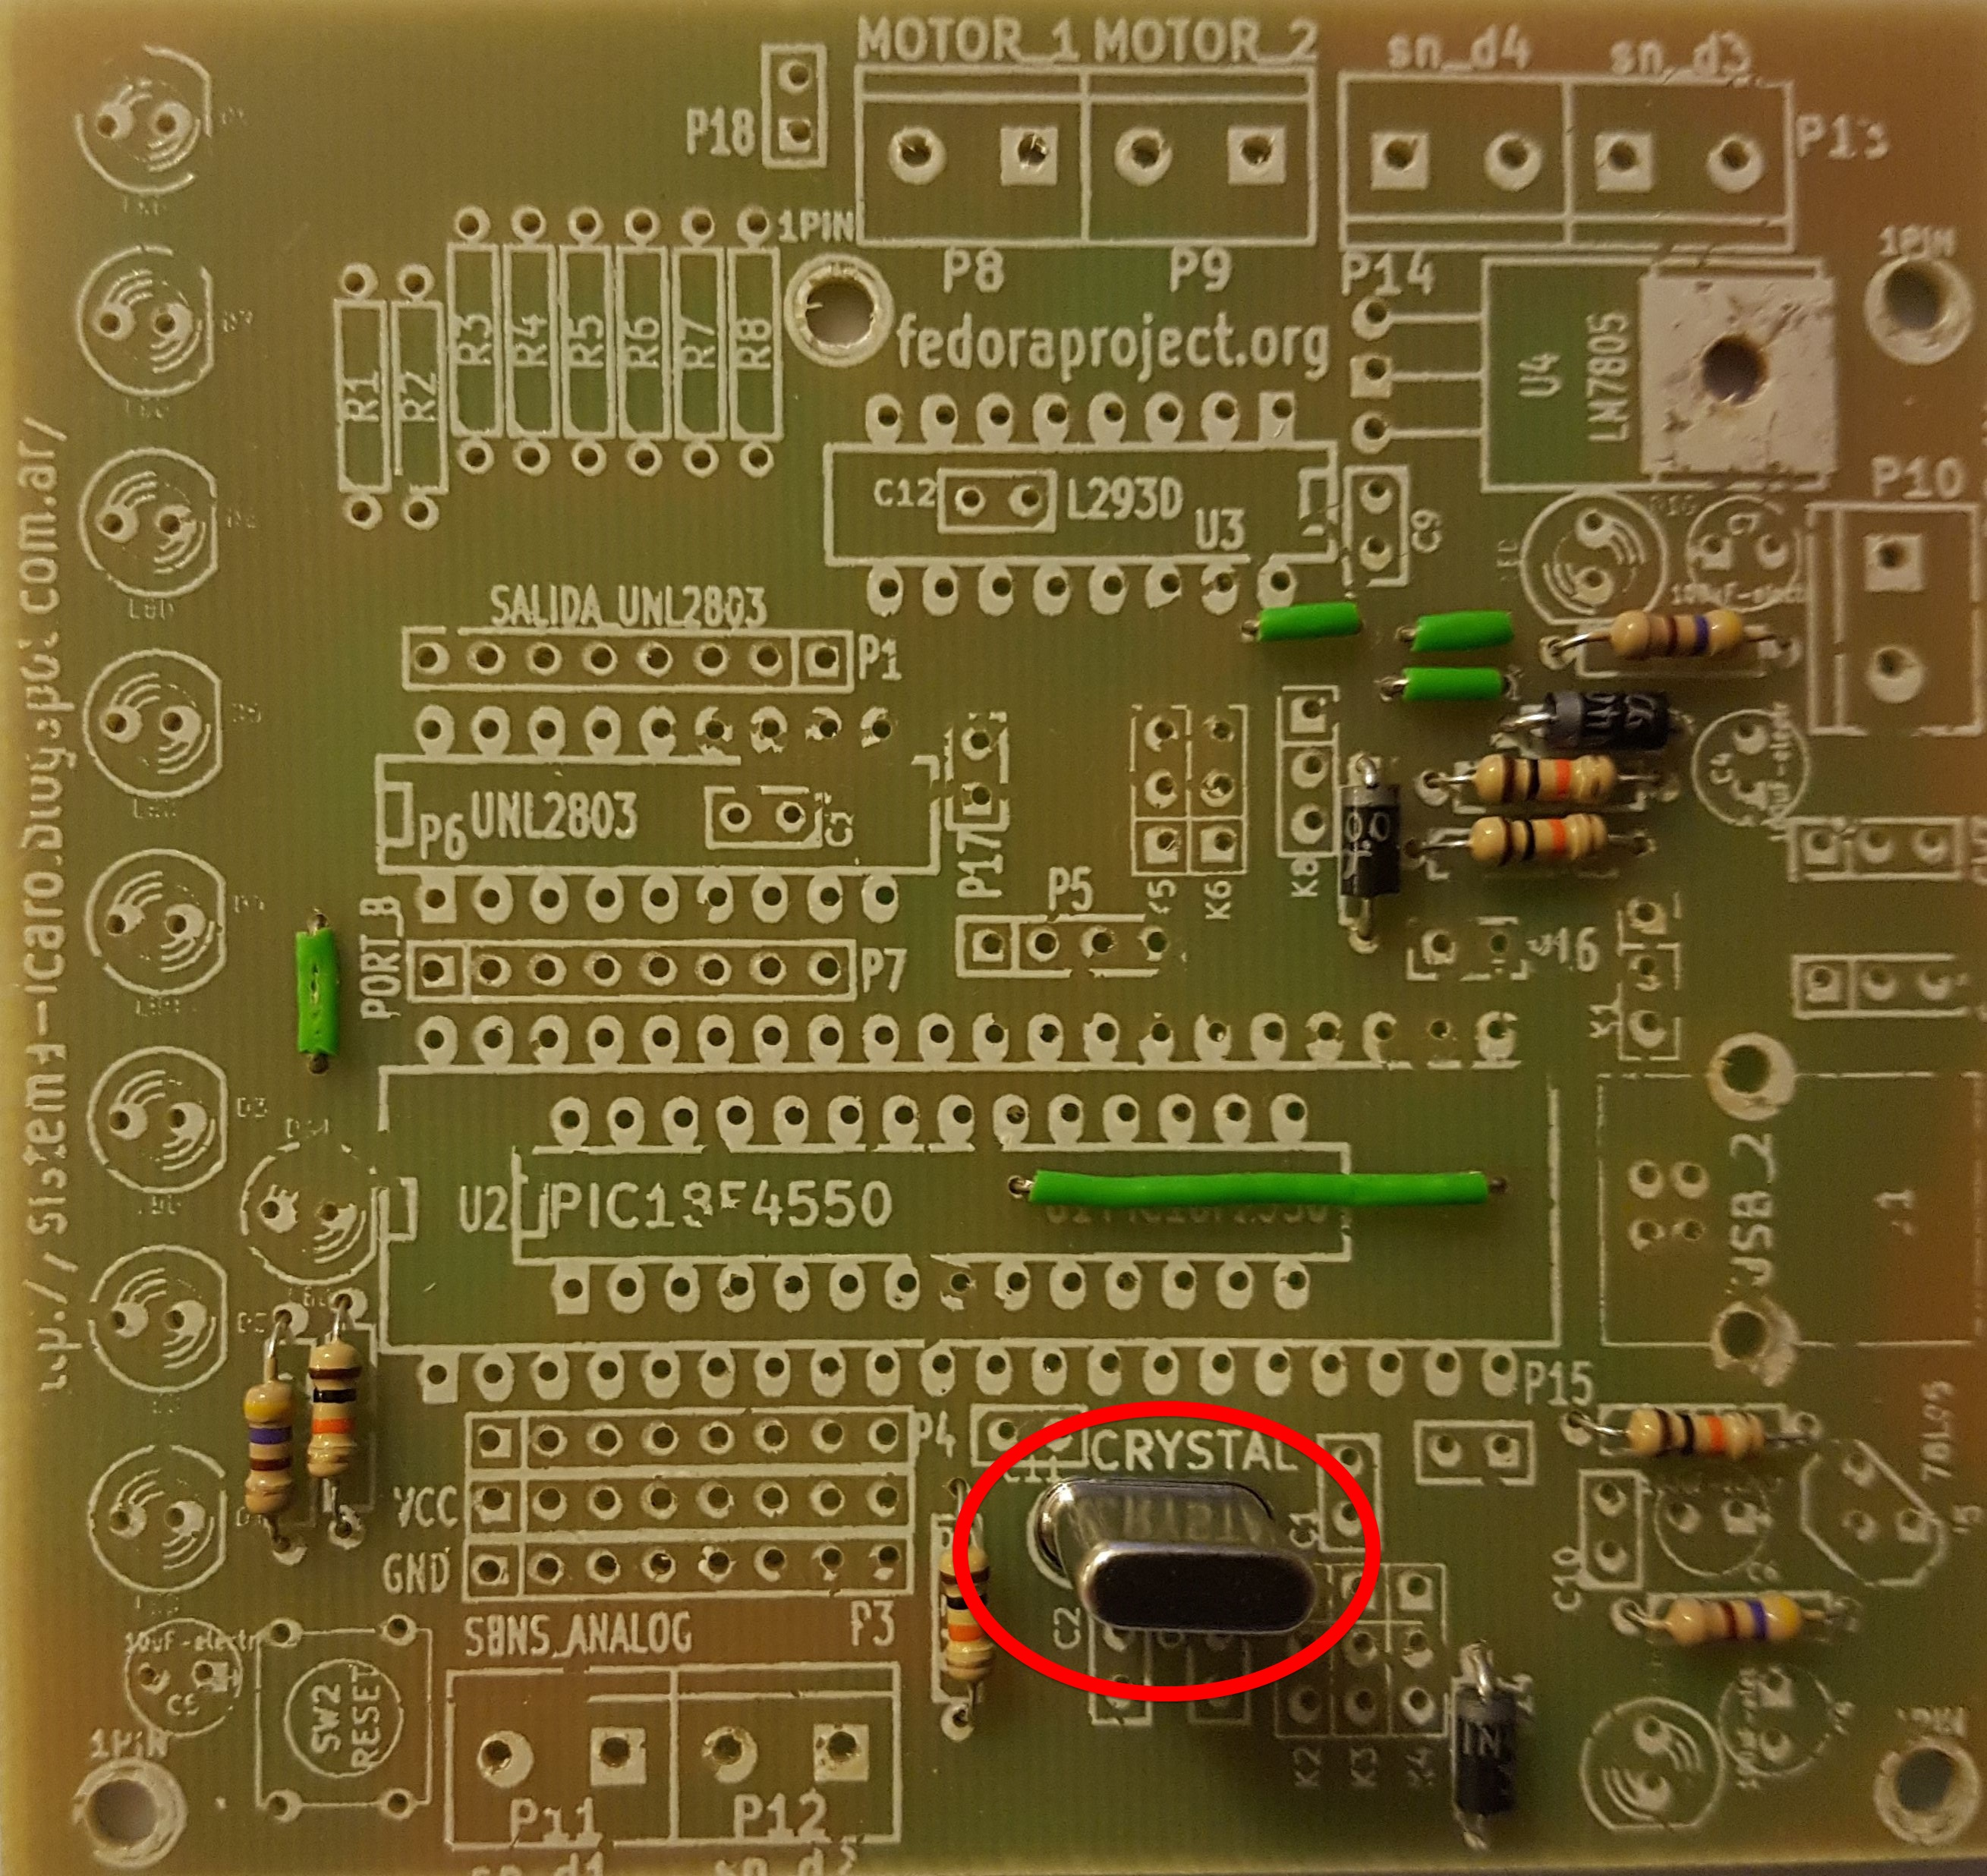
\includegraphics[width=0.8\linewidth]{Modulo_2/M2_1}
	\caption{Módulo 2 - Paso 1}
	\label{fig:M2_1}
\end{figure}

\newpage

\section{Paso 2:}

Push Botón (Reset). SW2

\begin{figure}[h]
	\centering
	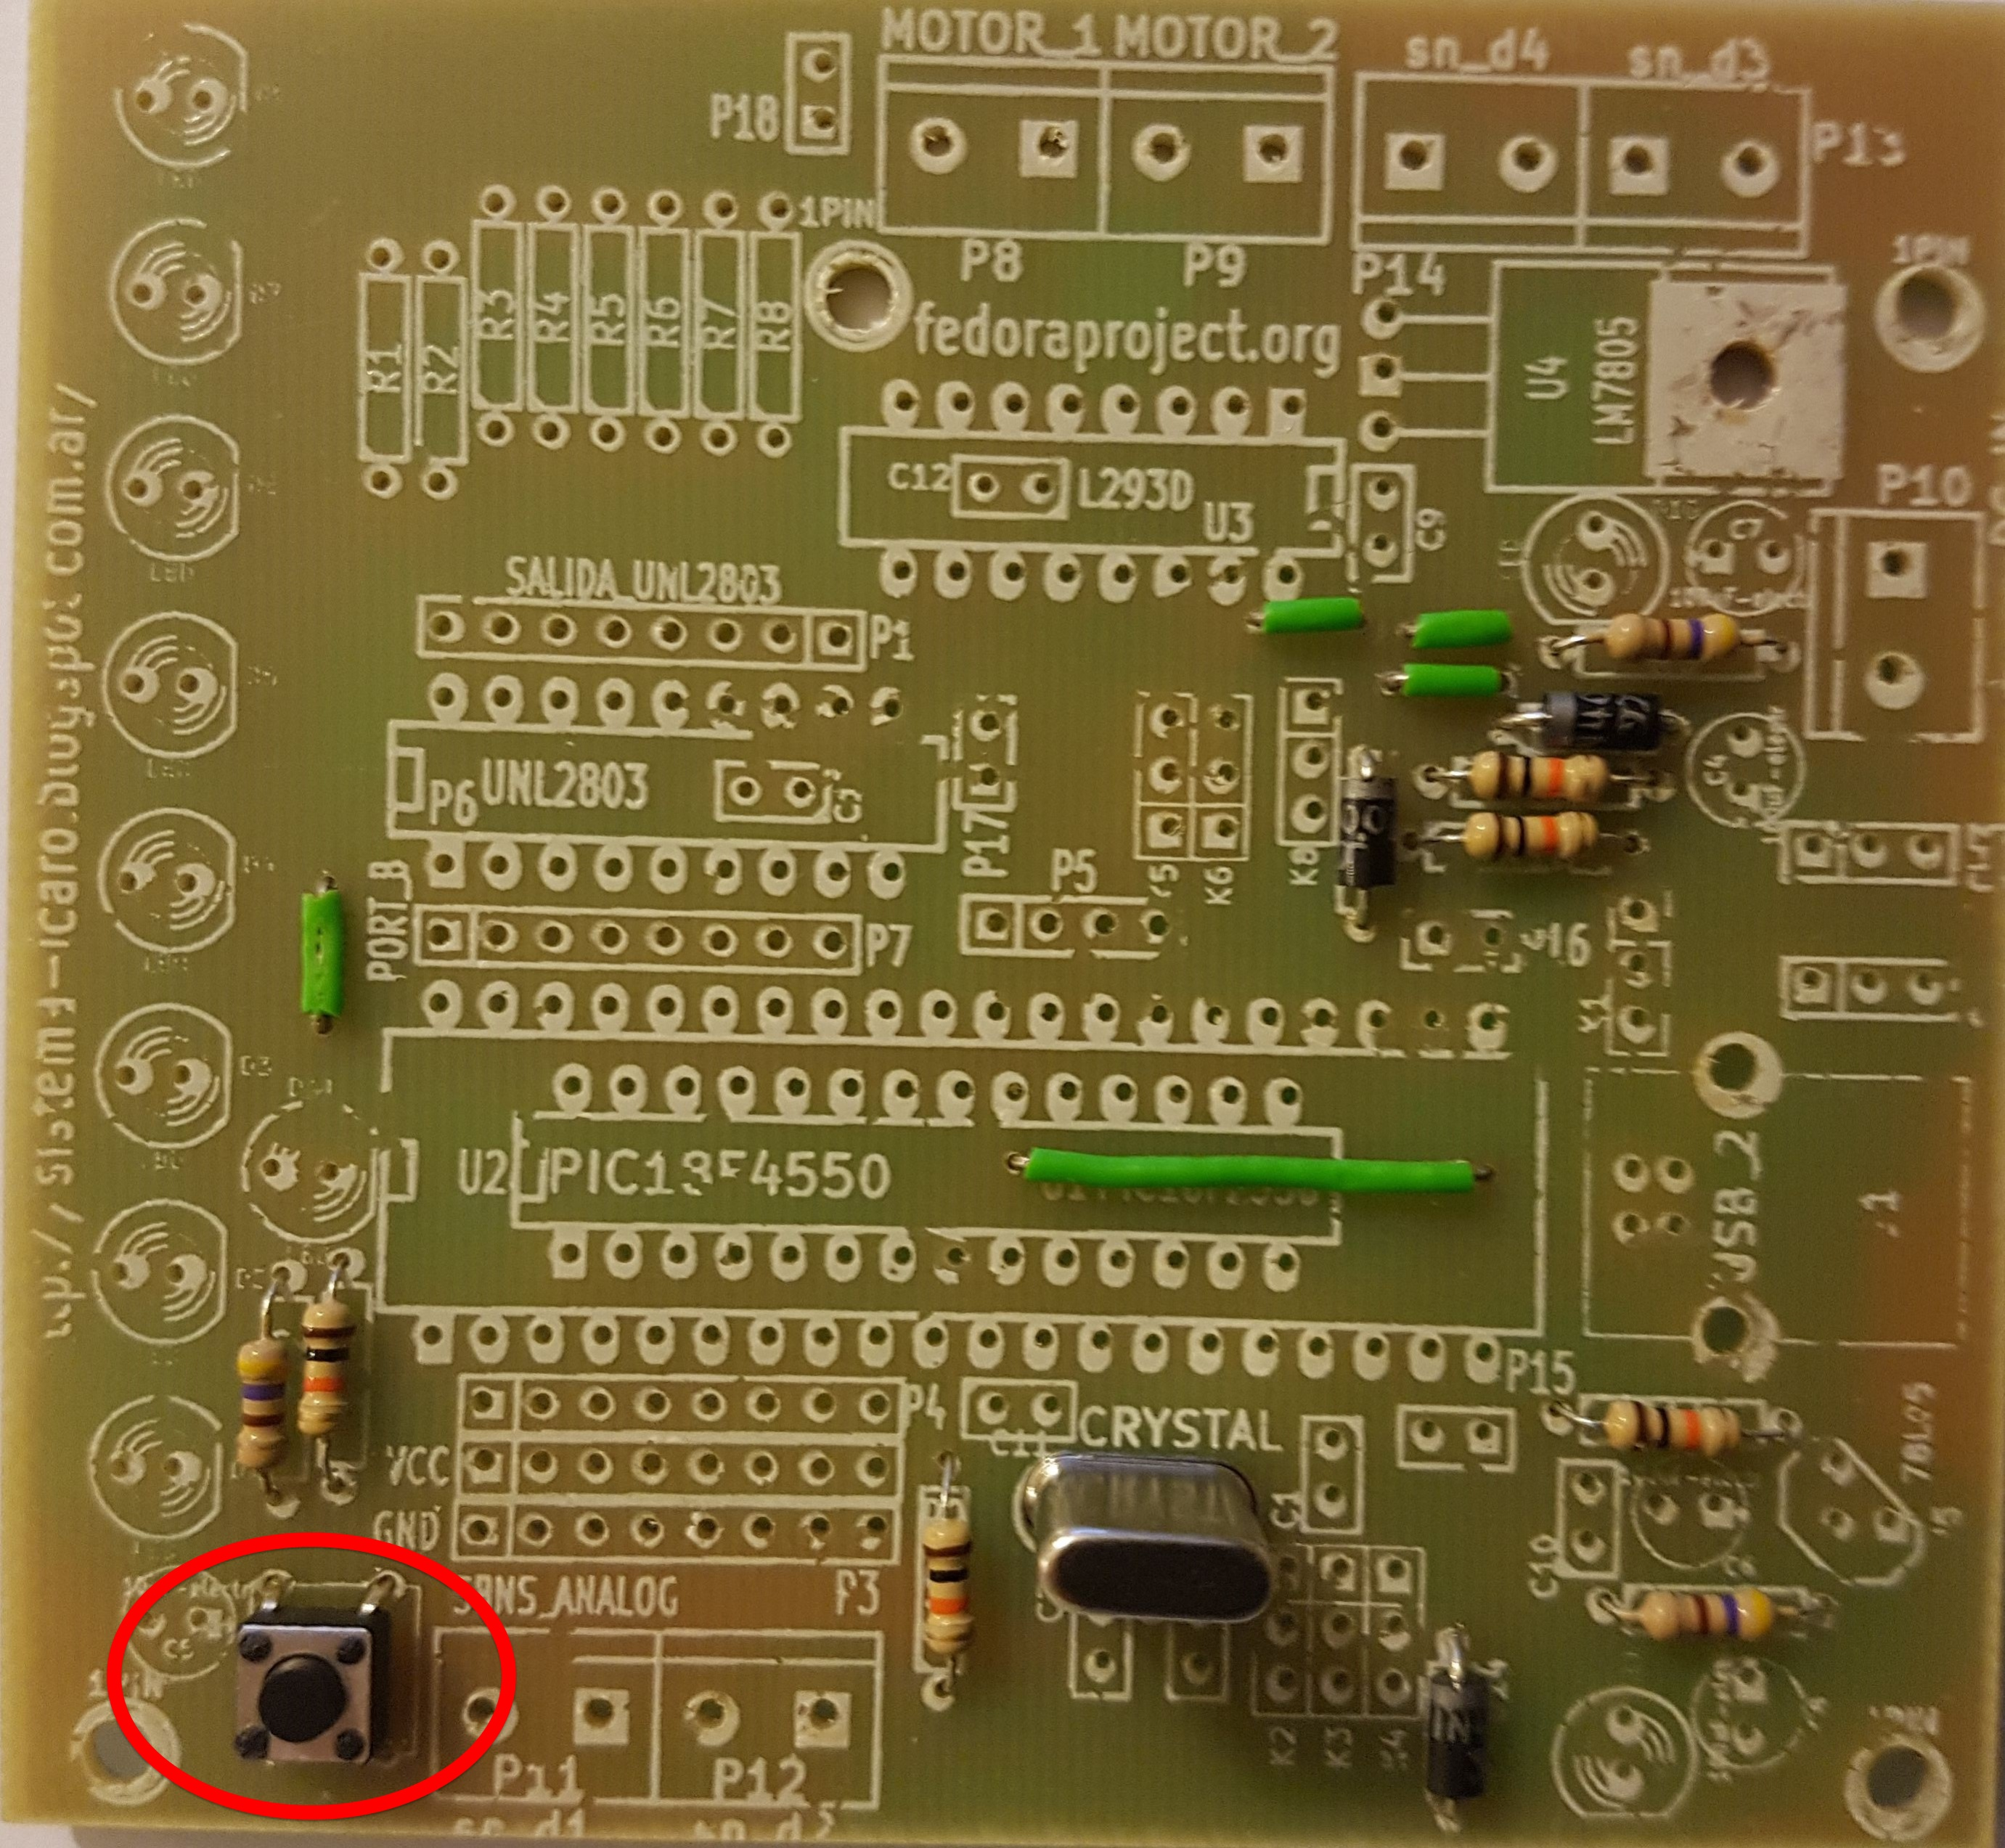
\includegraphics[width=0.8\linewidth]{Modulo_2/M2_2}
	\caption{Módulo 2 - Paso 2}
	\label{fig:M2_2}
\end{figure}

\newpage

\section{Paso 3:}

Instalar capacitor cerámico 220nF C1 

\begin{figure}[h]
	\centering
	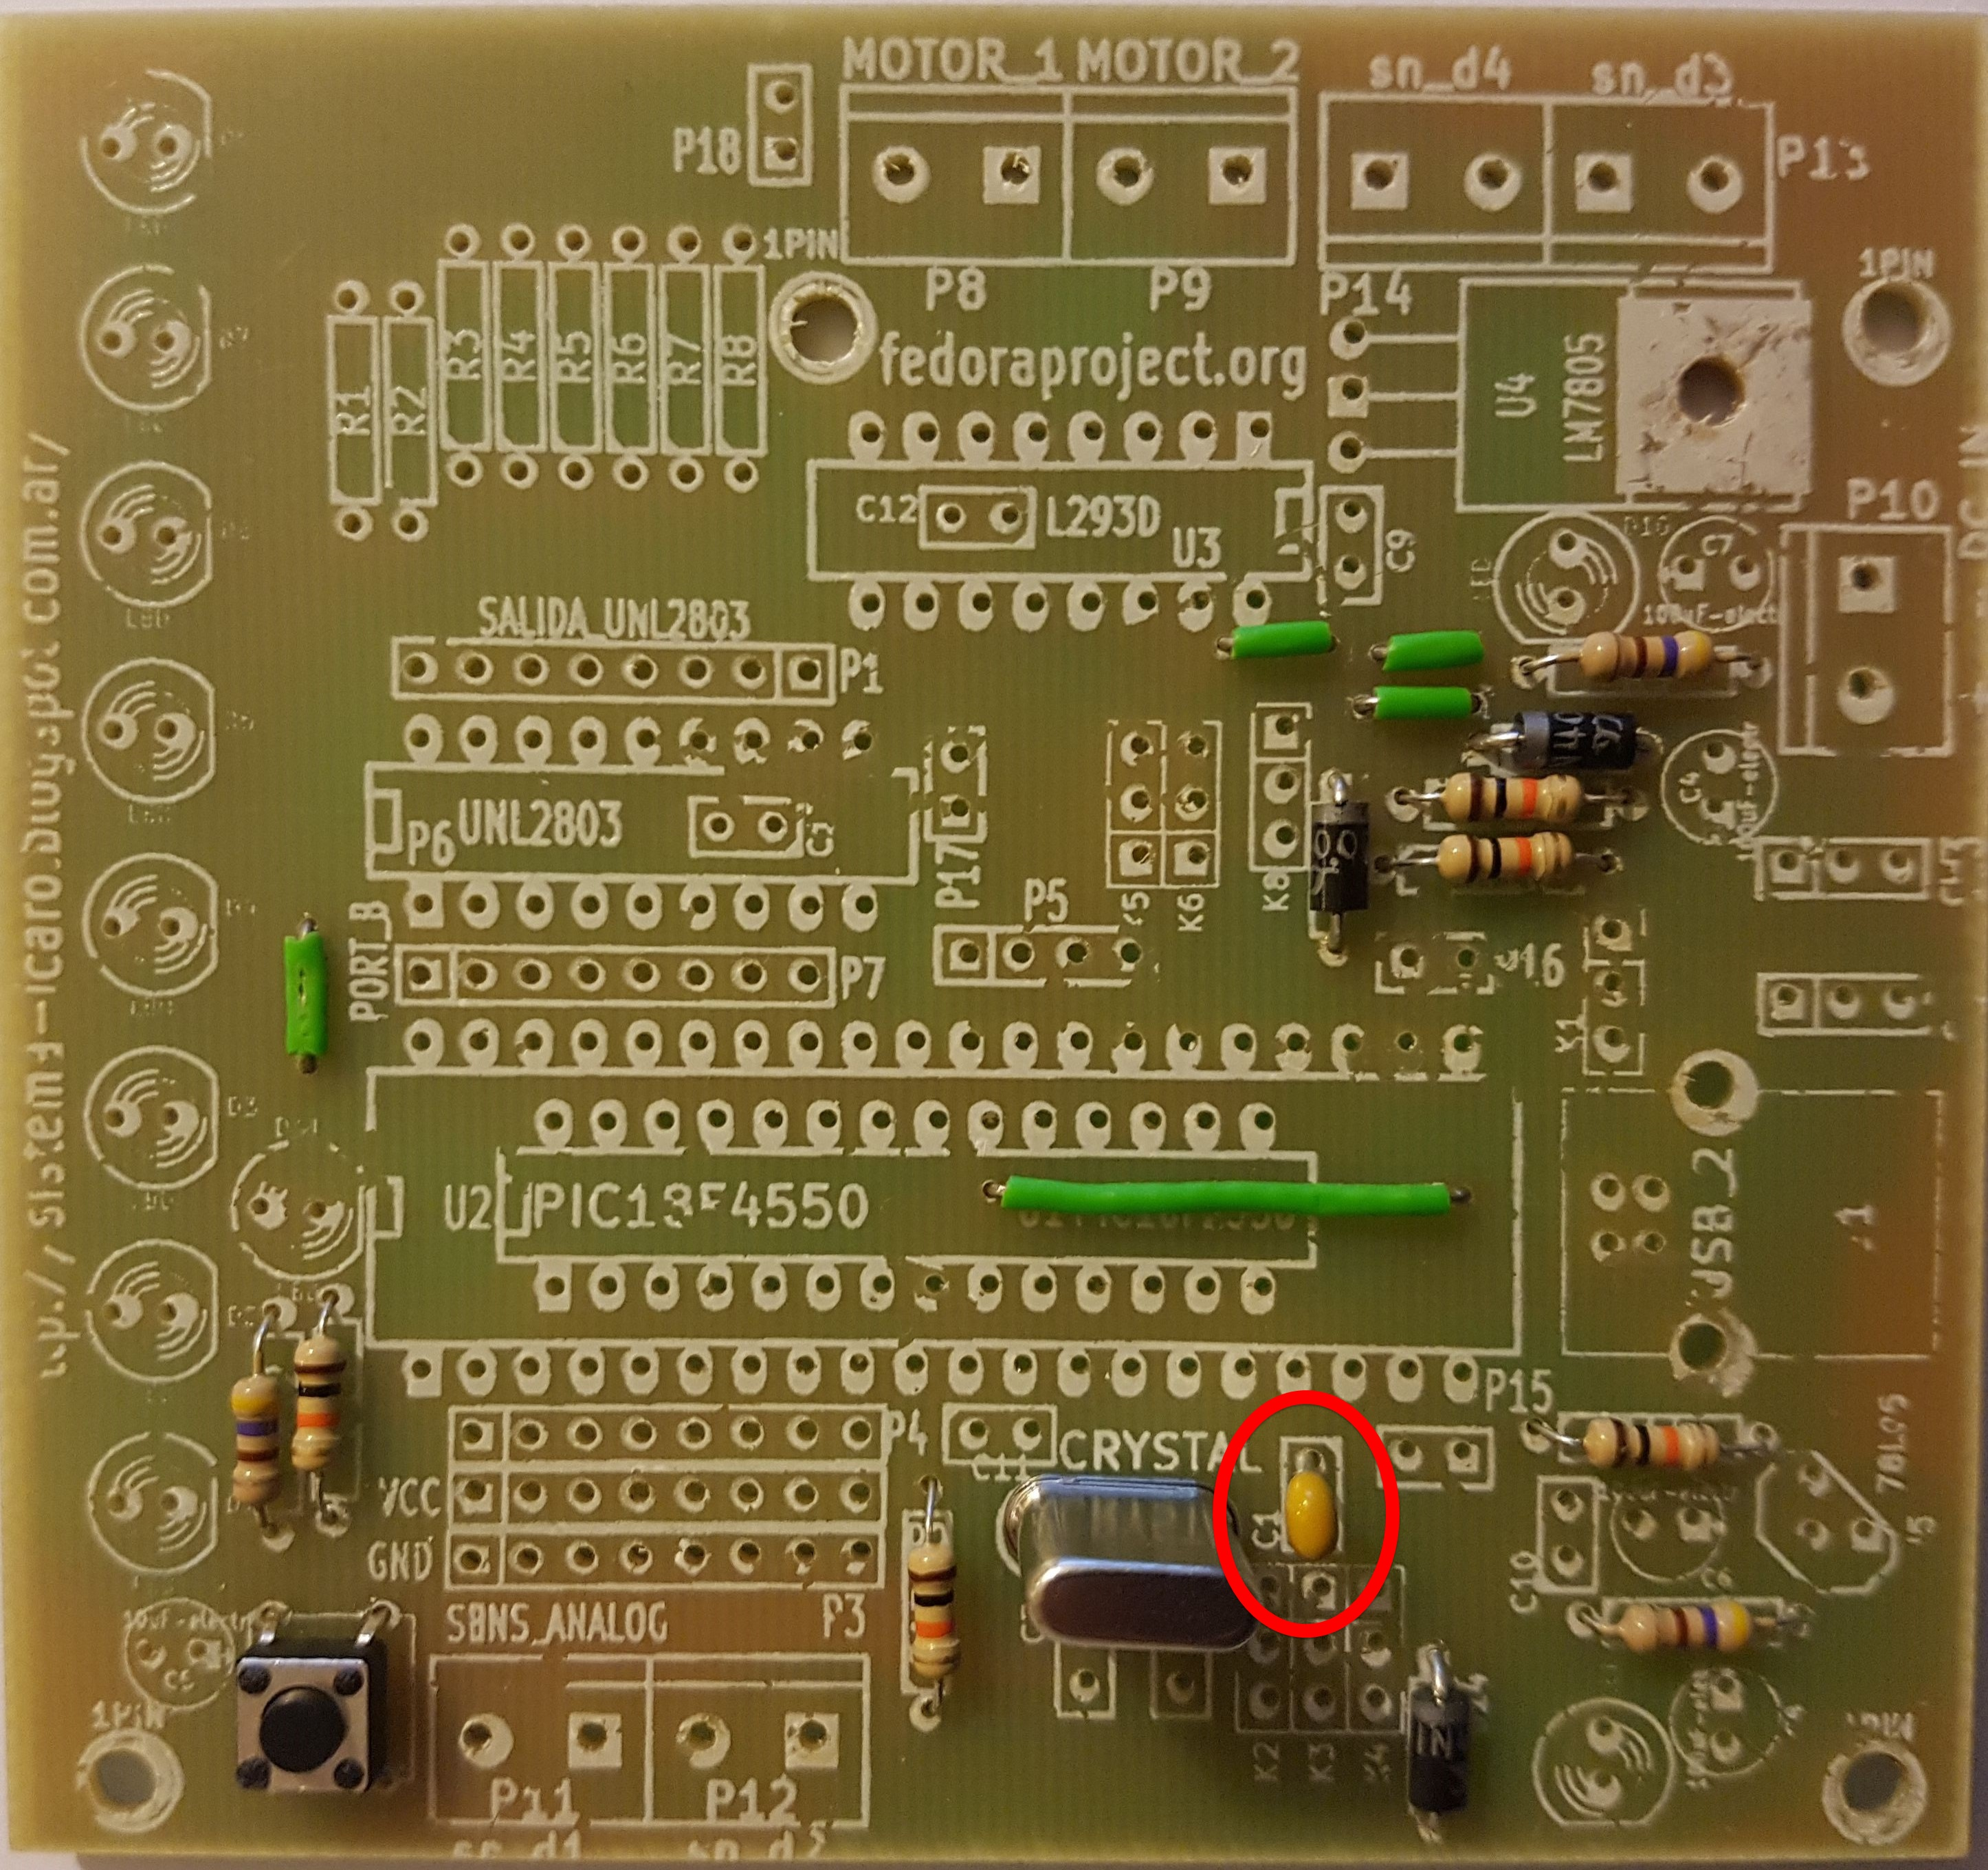
\includegraphics[width=0.8\linewidth]{Modulo_2/M2_3}
	\caption{Módulo 2 - Paso 3}
	\label{fig:M2_3}
\end{figure}

\newpage

\section{Paso 4:}

Instalar capacitor cerámico 0.1uF C11

\begin{figure}[h]
	\centering
	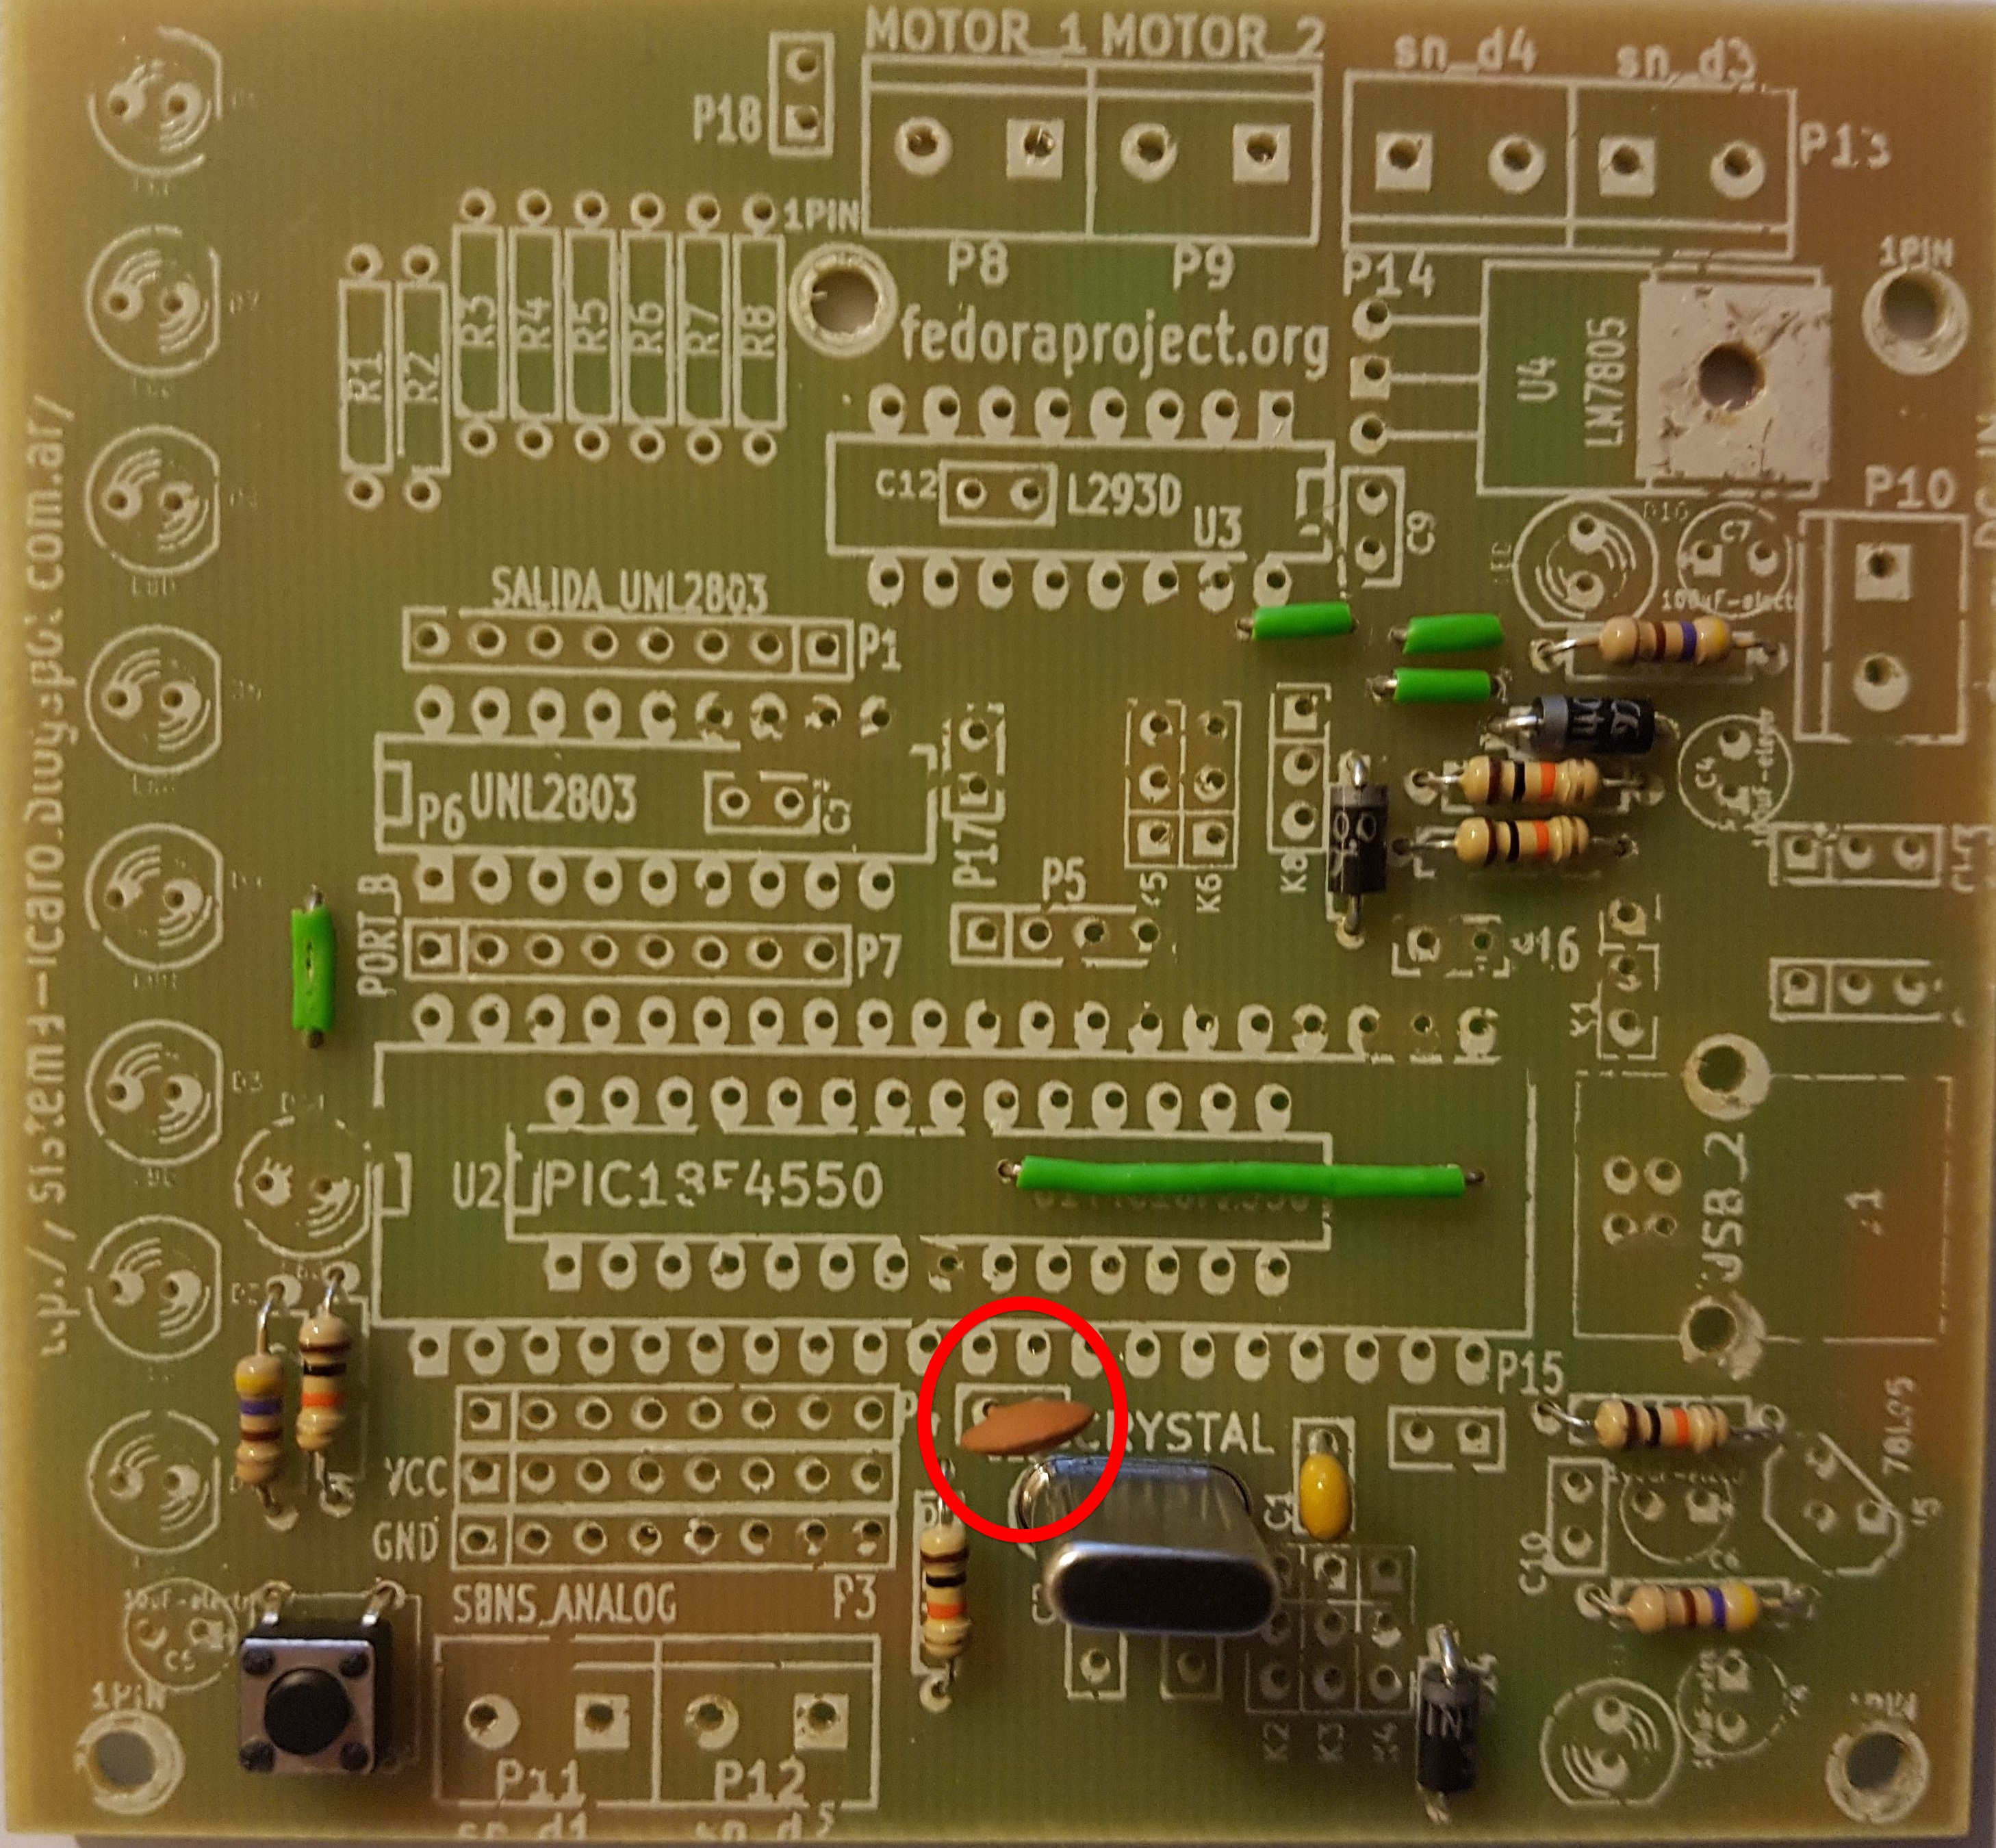
\includegraphics[width=0.8\linewidth]{Modulo_2/M2_4}
	\caption{Módulo 2 - Paso 4}
	\label{fig:M2_4}
\end{figure}

\newpage

\section{Paso 5:}

Instalar capacitadores cerámicos 22pF C2 y C3

\begin{figure}[h]
	\centering
	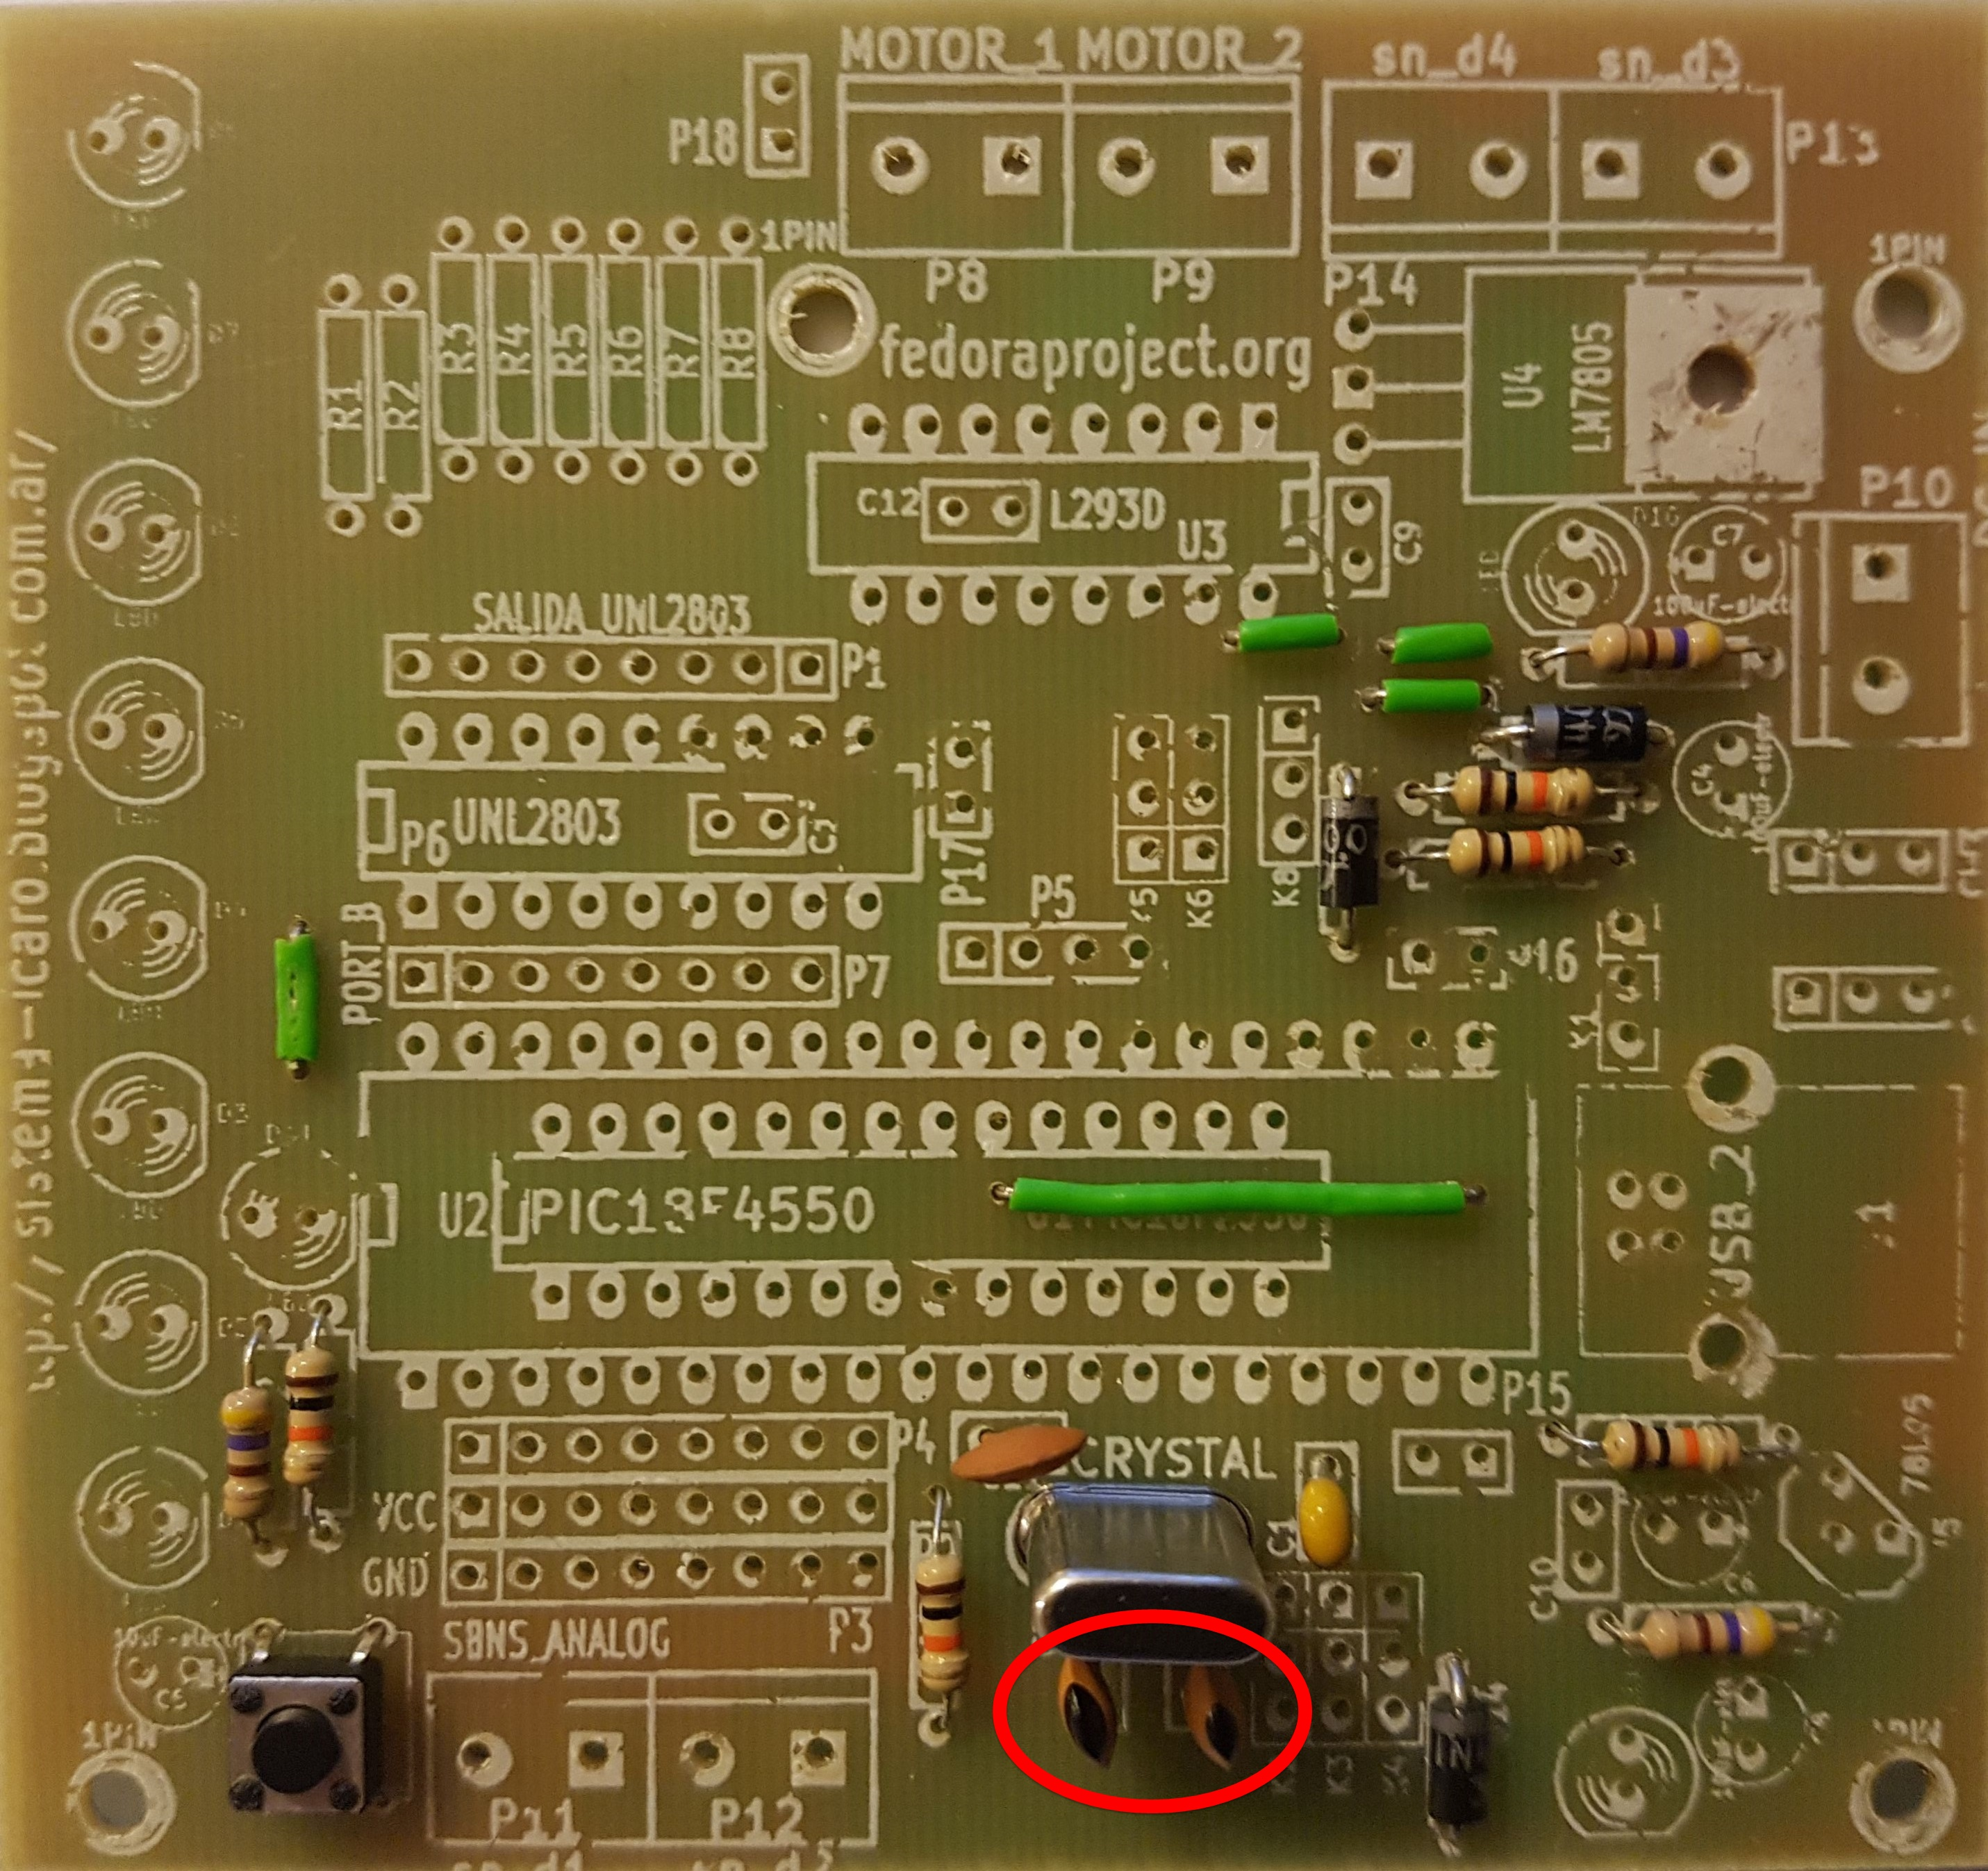
\includegraphics[width=0.8\linewidth]{Modulo_2/M2_5}
	\caption{Módulo 2 - Paso 5}
	\label{fig:M2_5}
\end{figure}

\newpage

\section{Paso 6:}

Instalar Sócalo de 40 patas (20x2) U2 Tomar en cuenta alinear la muesca del diagrama de la placa con la muesca del zócalo.

\begin{figure}[h]
	\centering
	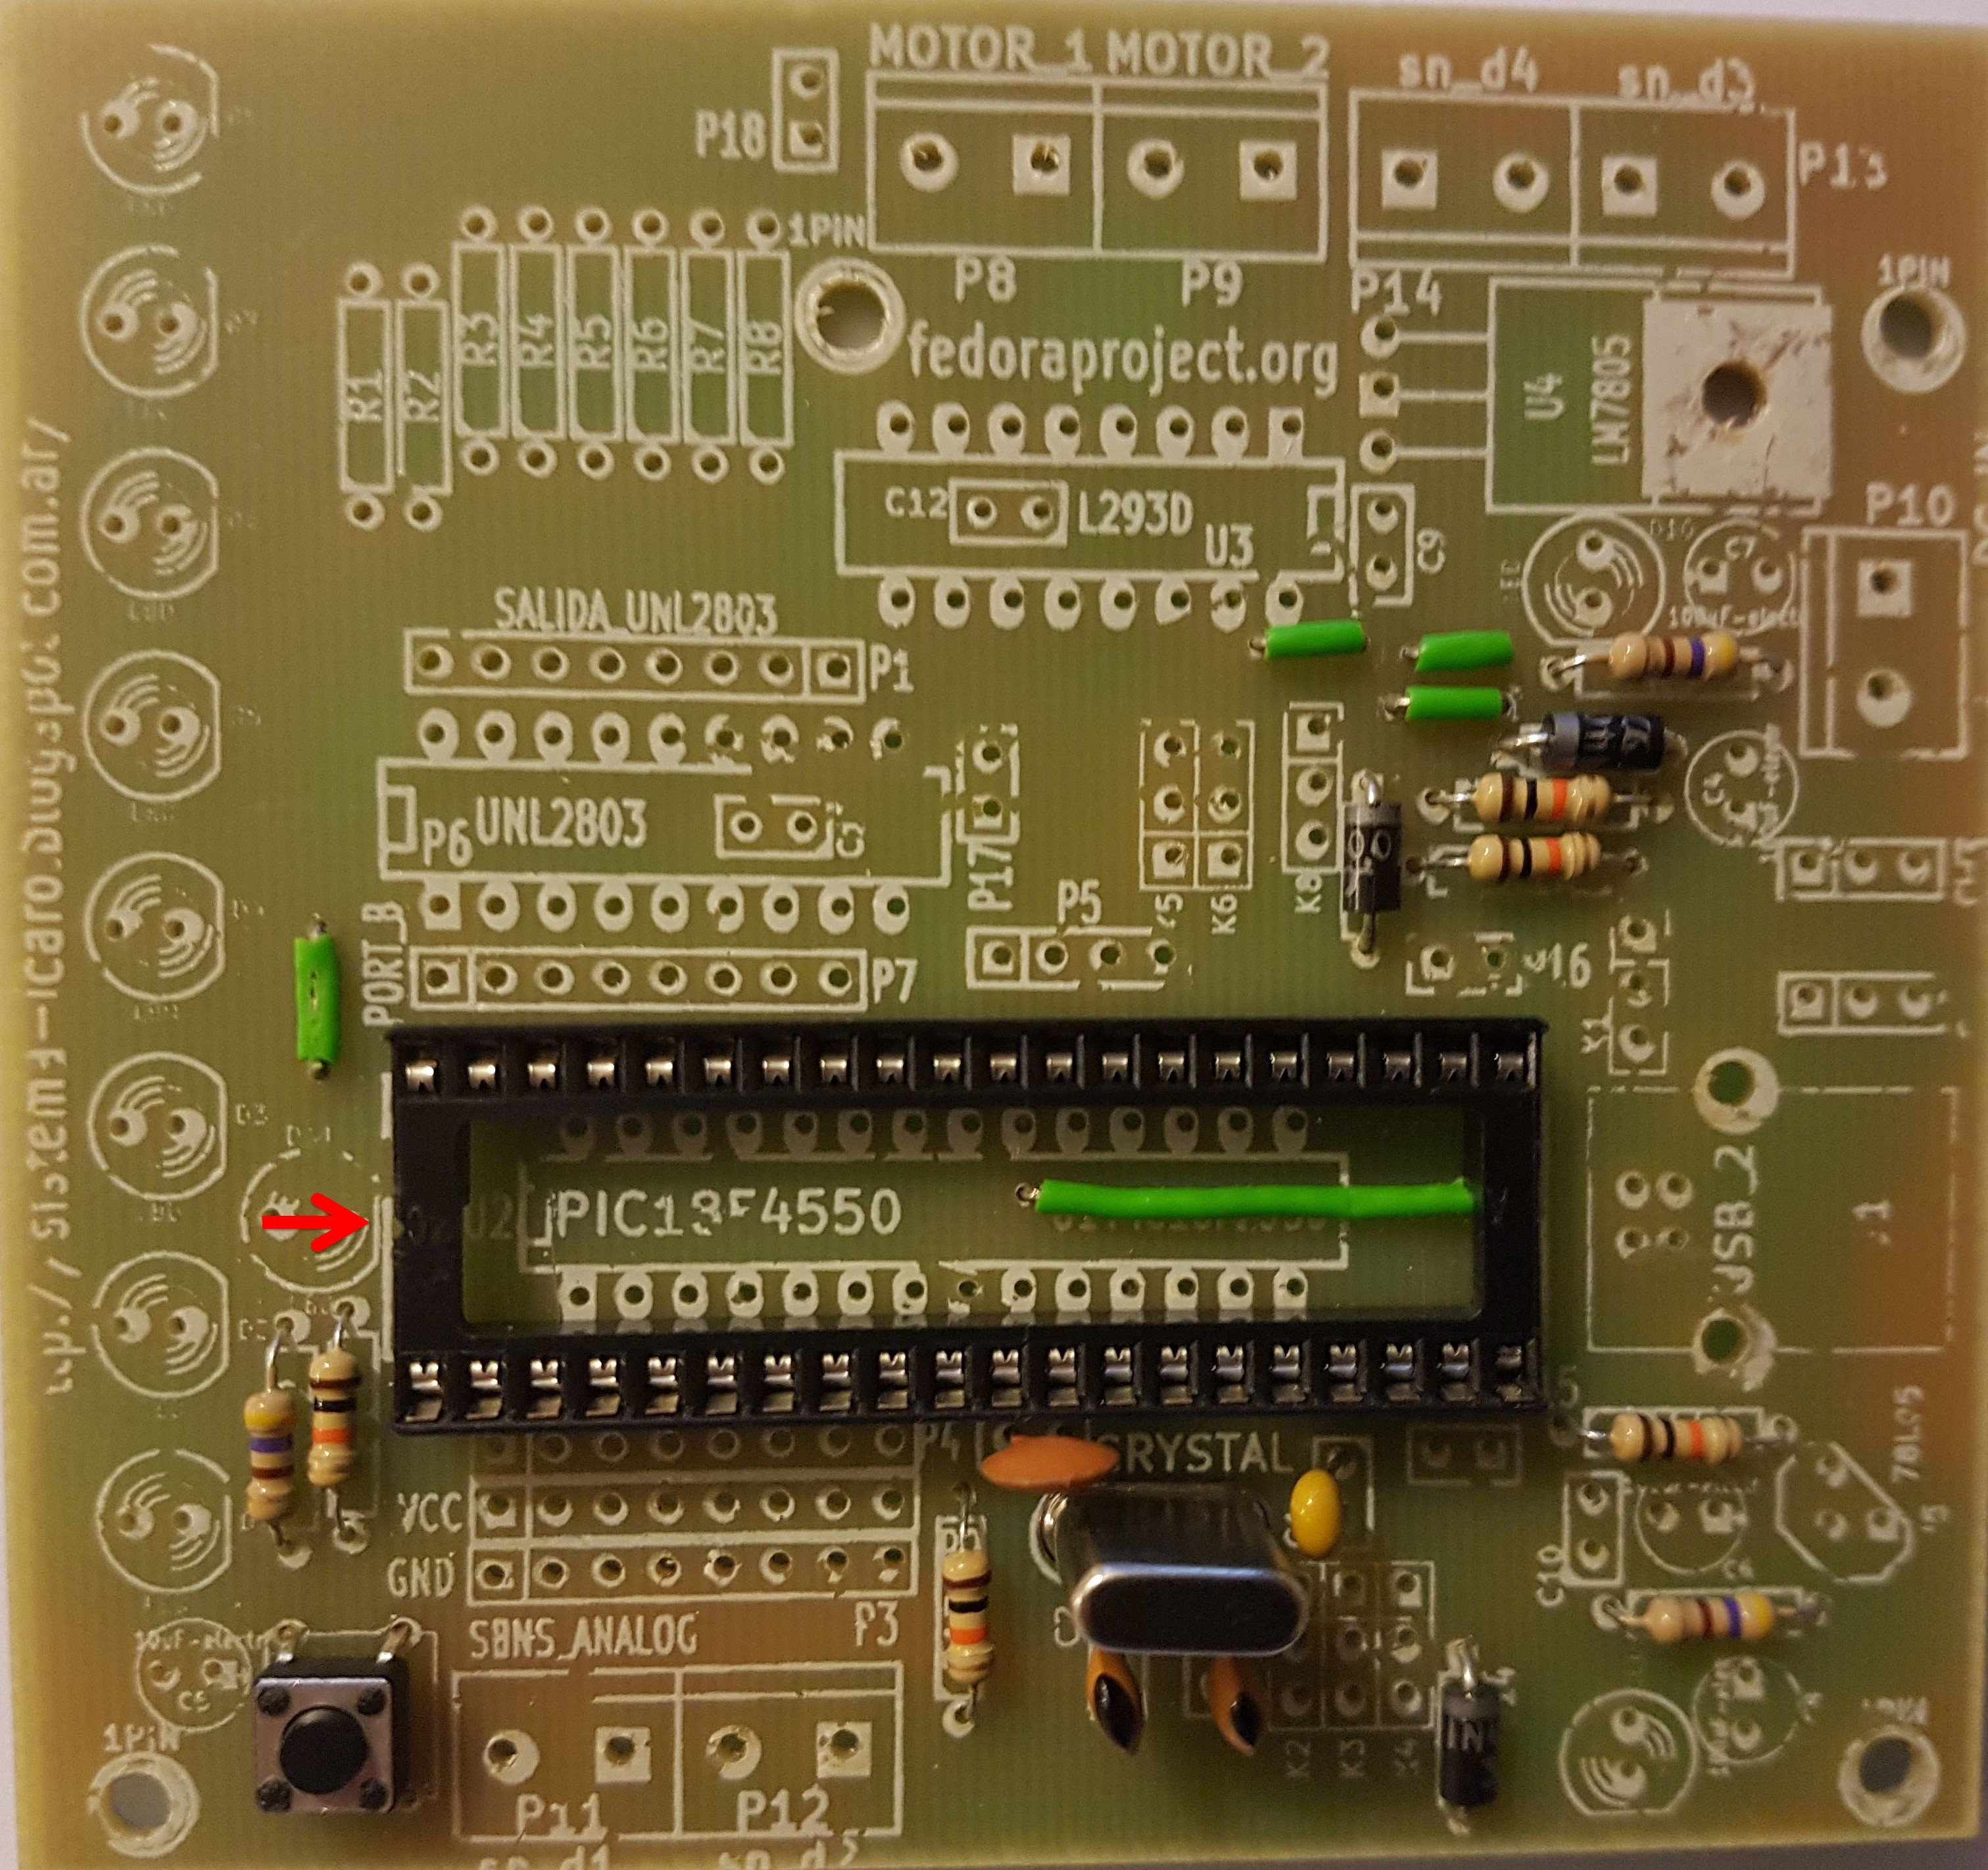
\includegraphics[width=0.8\linewidth]{Modulo_2/M2_6}
	\caption{Módulo 2 - Paso 6}
	\label{fig:M2_6}
\end{figure}

\newpage

\section{Paso 7:}

Instalar led del microcontrolador. D11 (Se recomienda color rojo)

\begin{figure}[h]
	\centering
	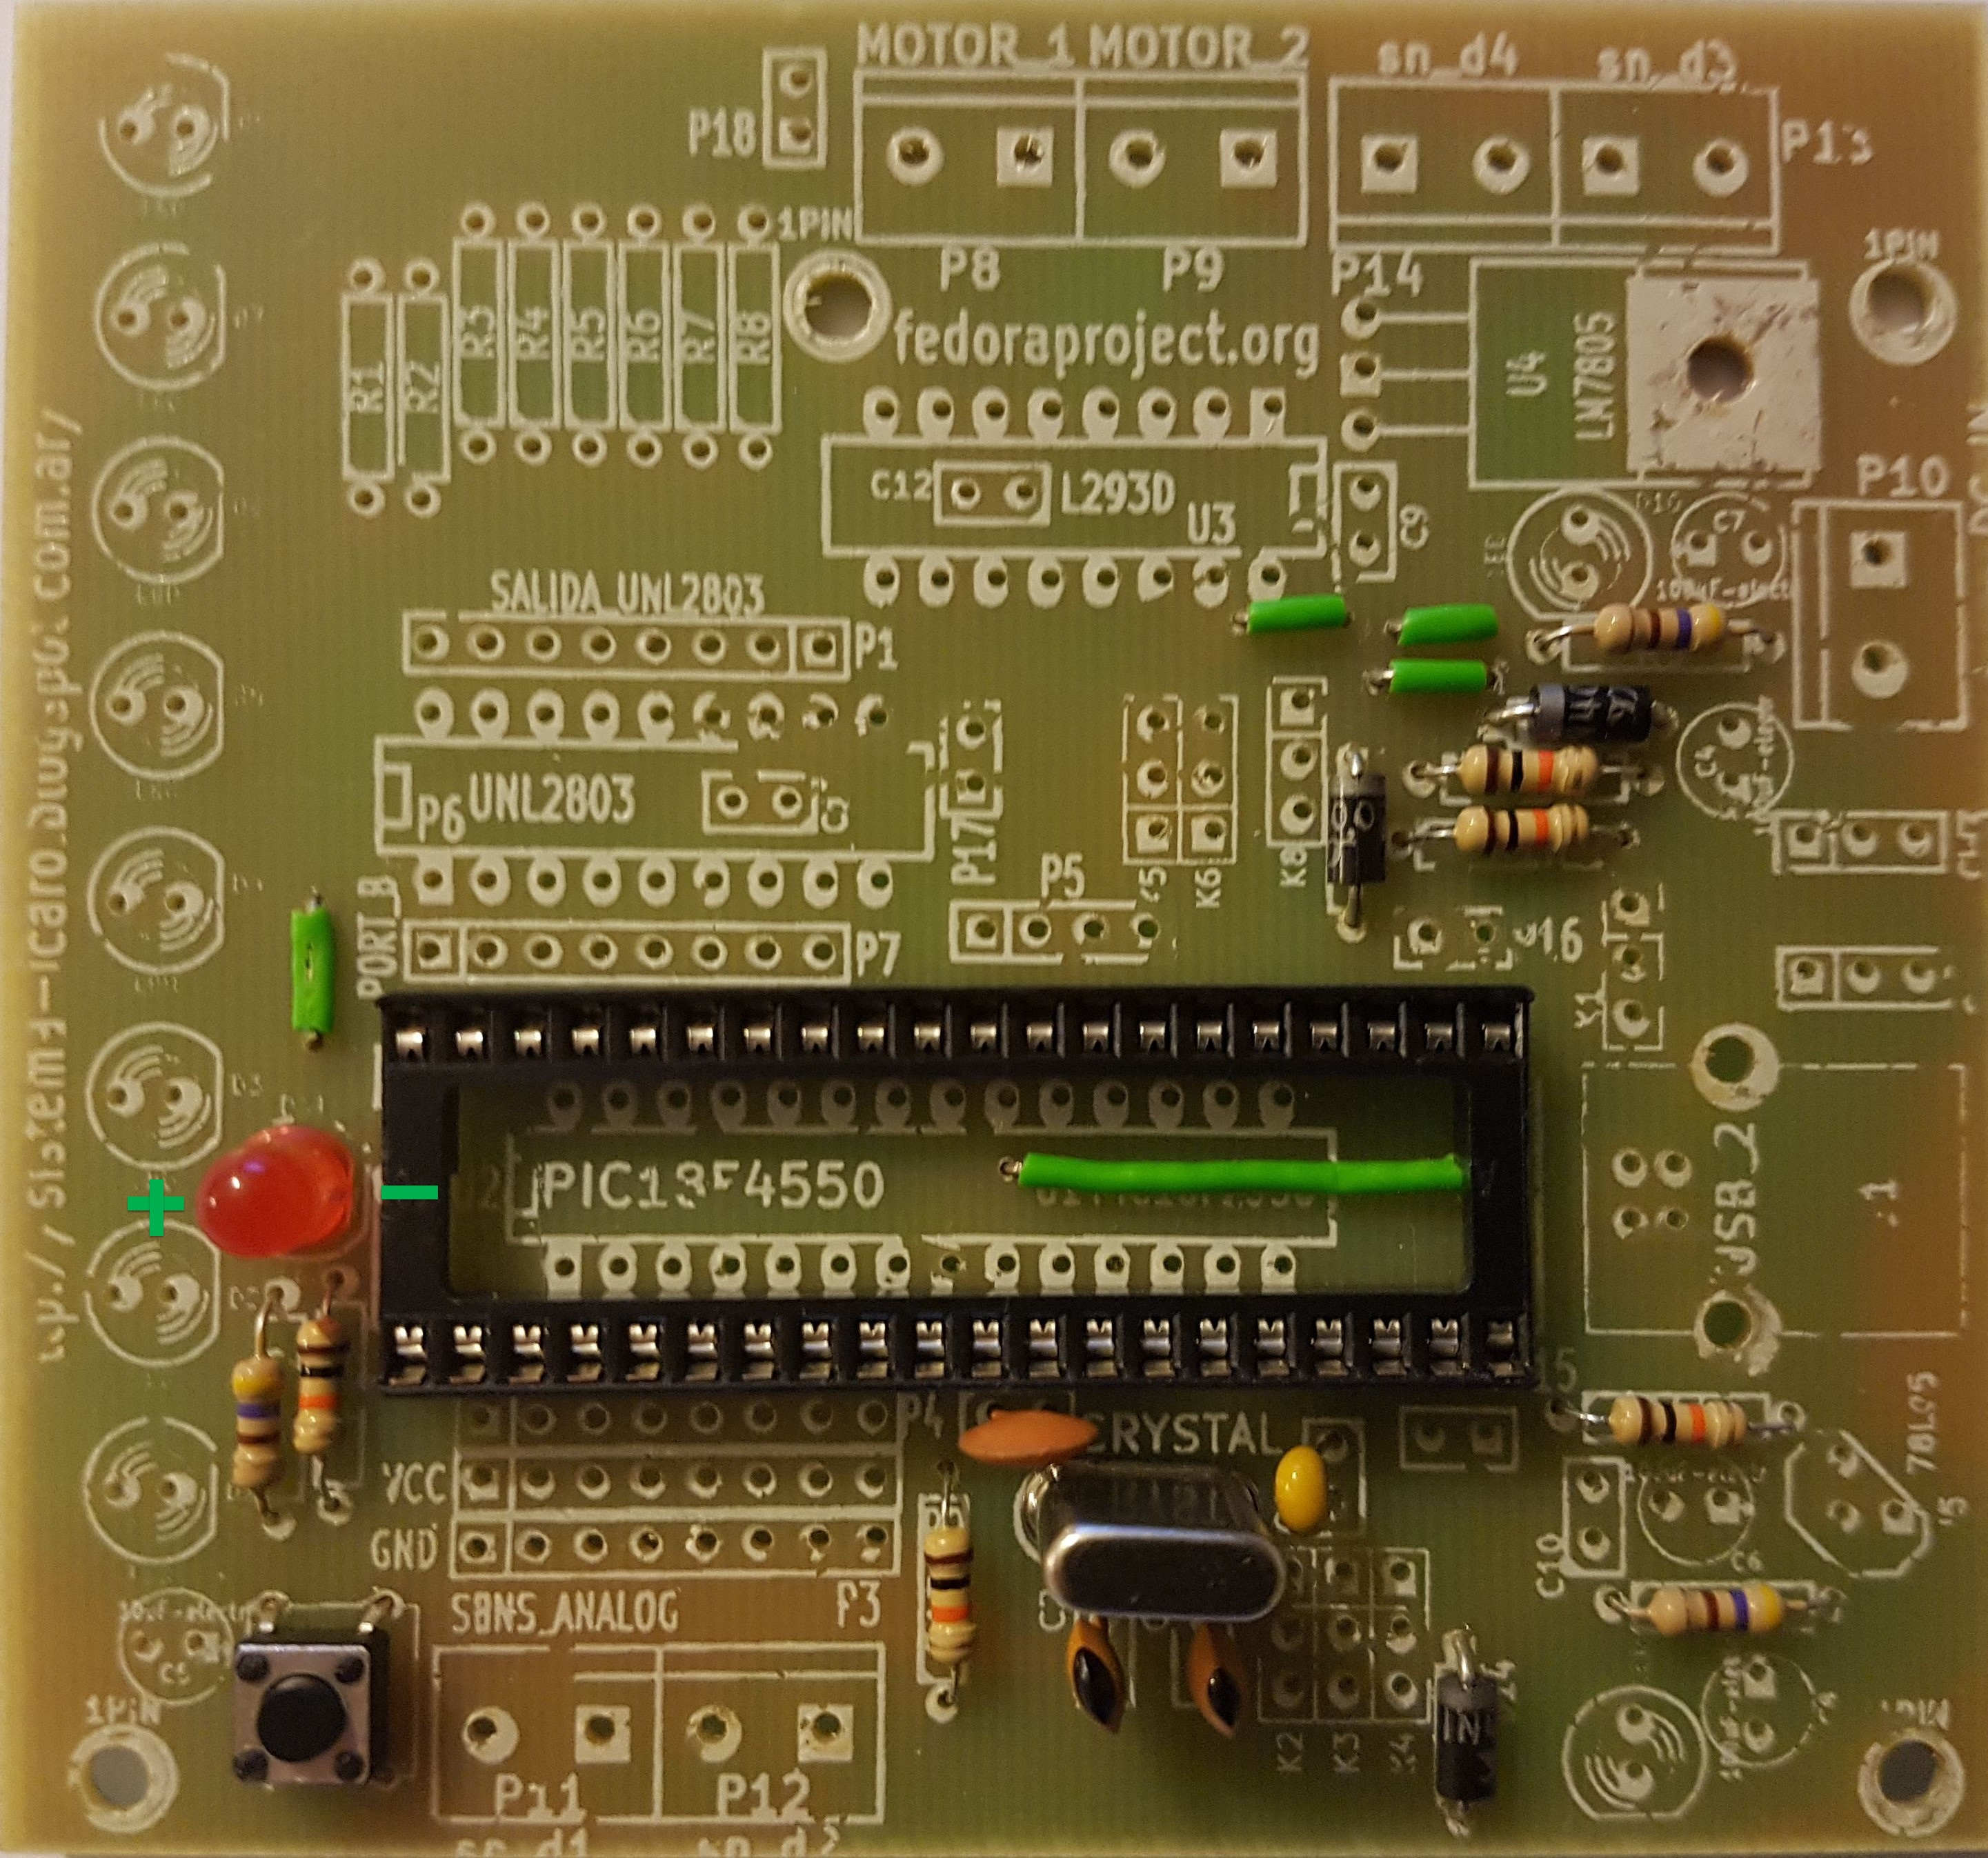
\includegraphics[width=0.8\linewidth]{Modulo_2/M2_7}
	\caption{Módulo 2 - Paso 7}
	\label{fig:M2_7}
\end{figure}

\newpage

\section{Paso 8:}

Instalar pines machos K1

\begin{figure}[h]
	\centering
	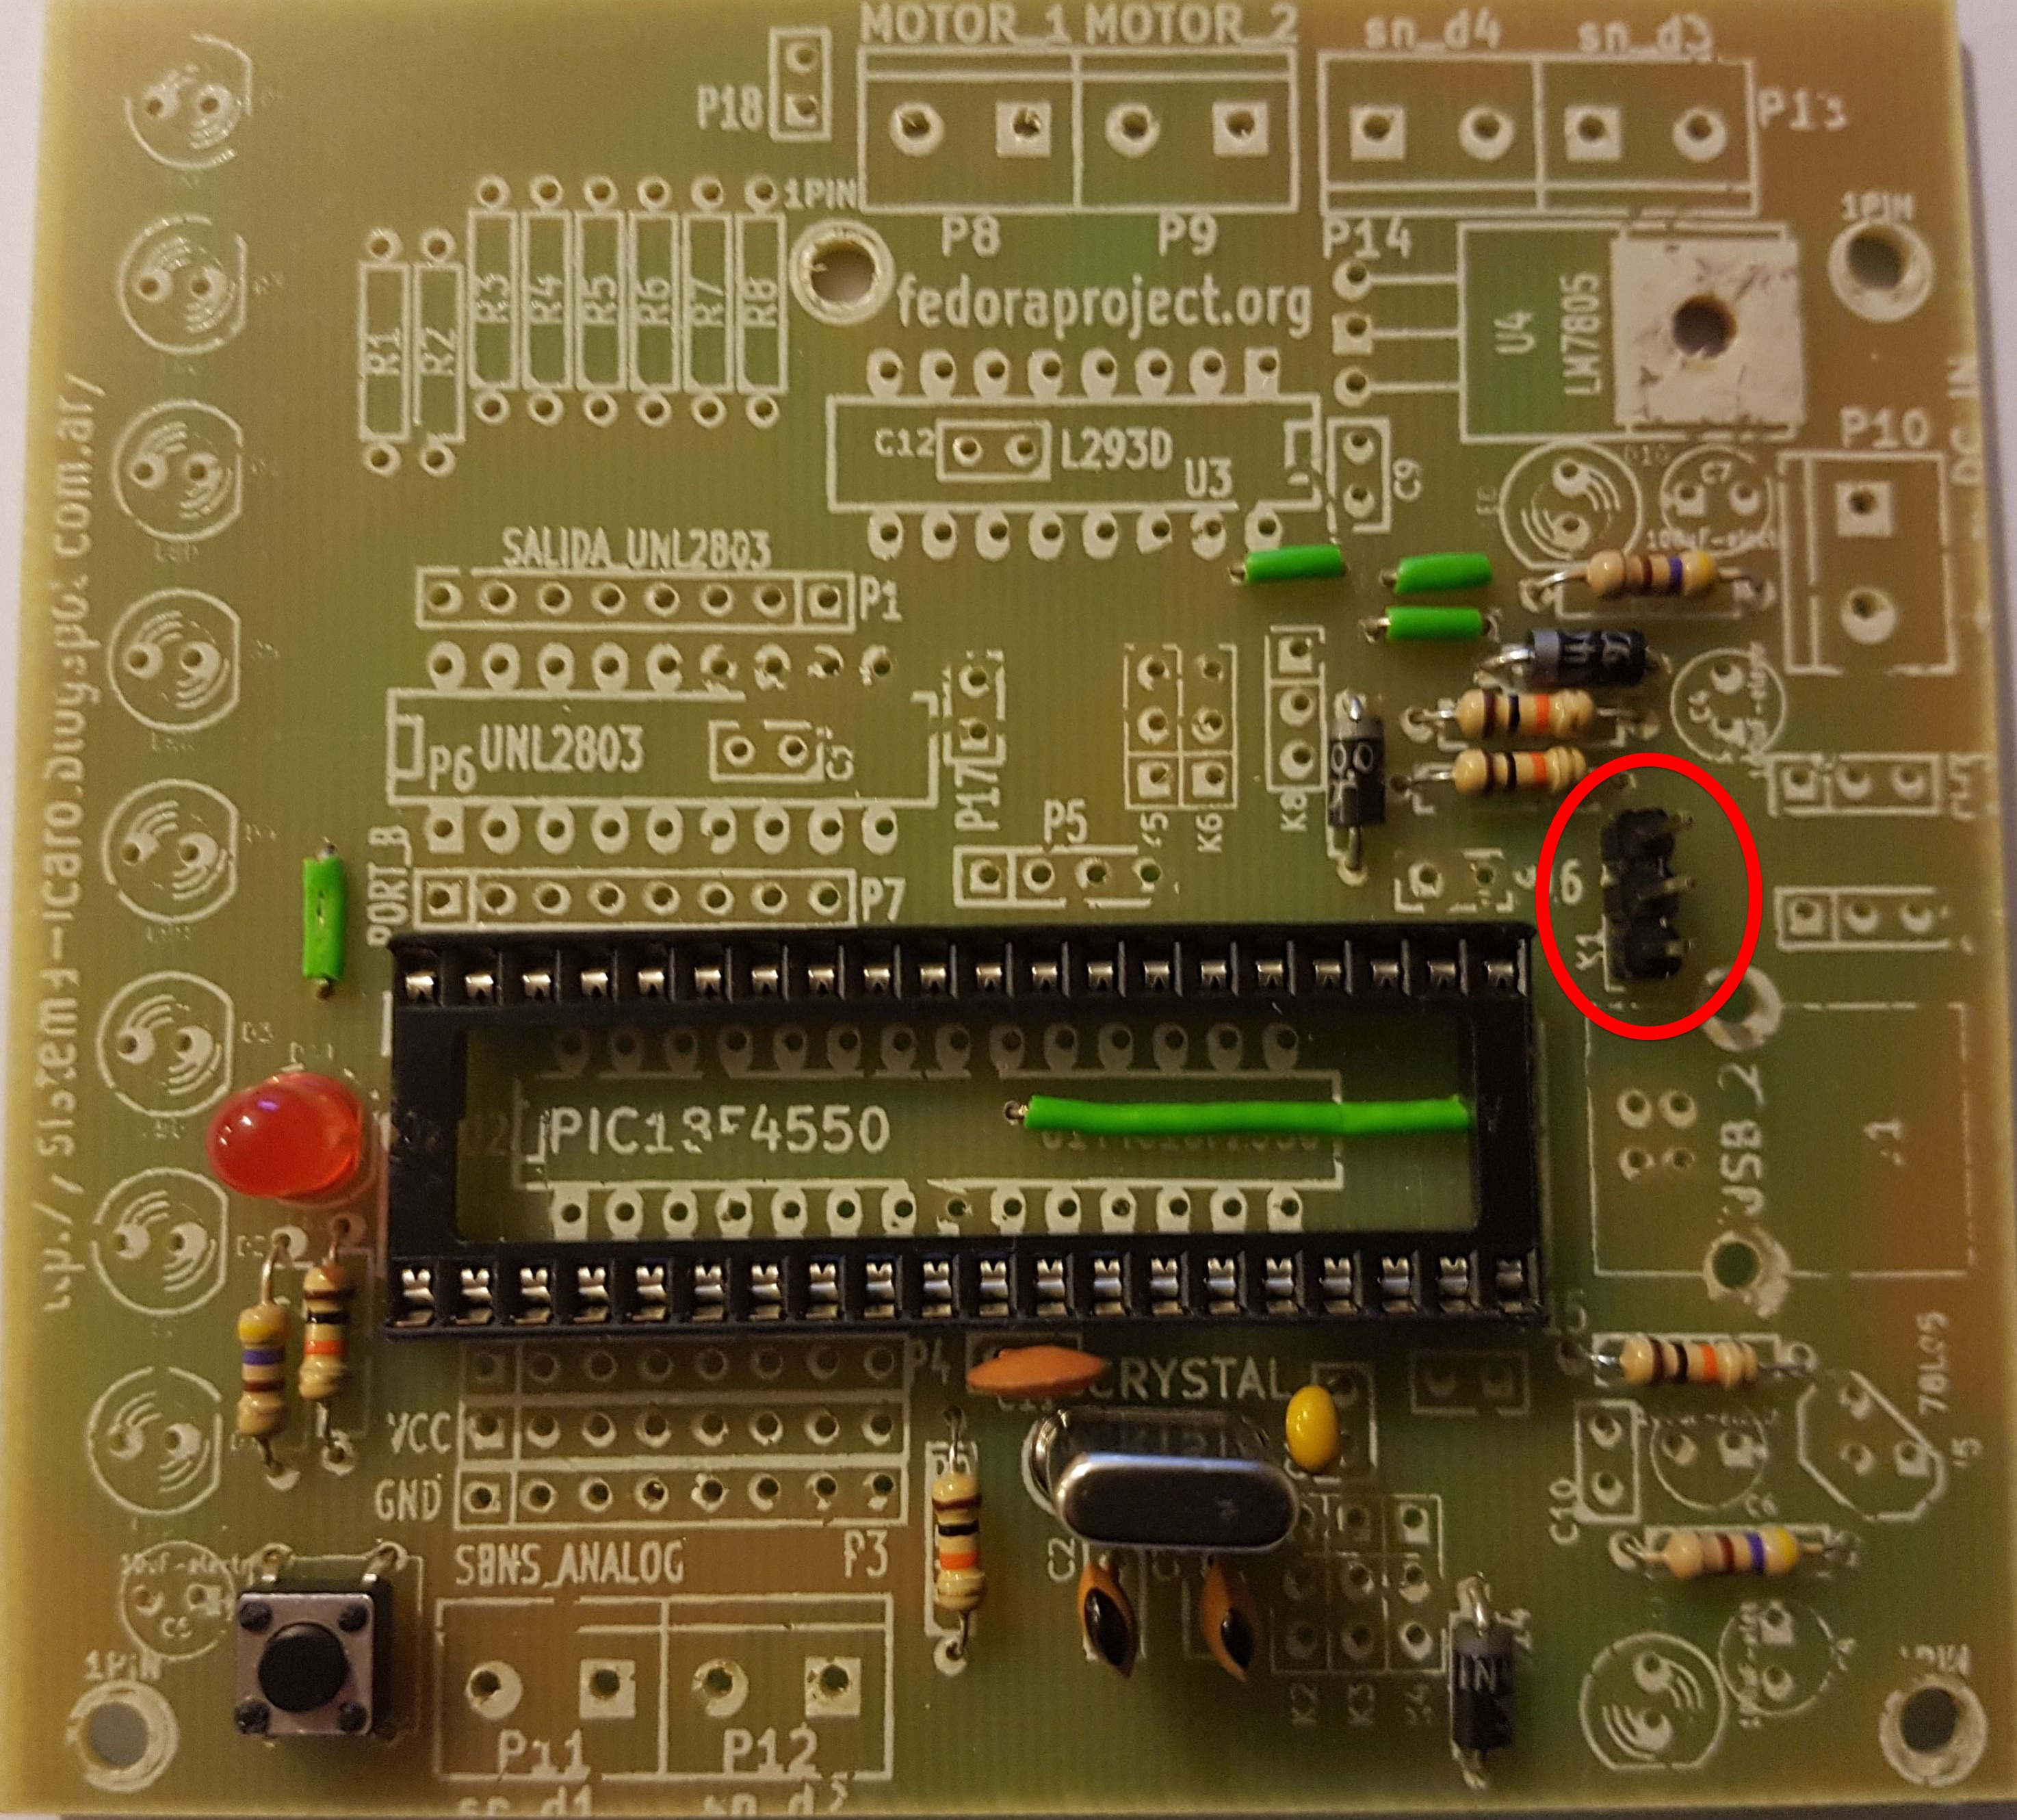
\includegraphics[width=0.8\linewidth]{Modulo_2/M2_8}
	\caption{Módulo 2 - Paso 8}
	\label{fig:M2_8}
\end{figure}

\newpage

\section{Paso 9:}

Instalar capacitor electrolítico 10uF. C5

\begin{figure}[h]
	\centering
	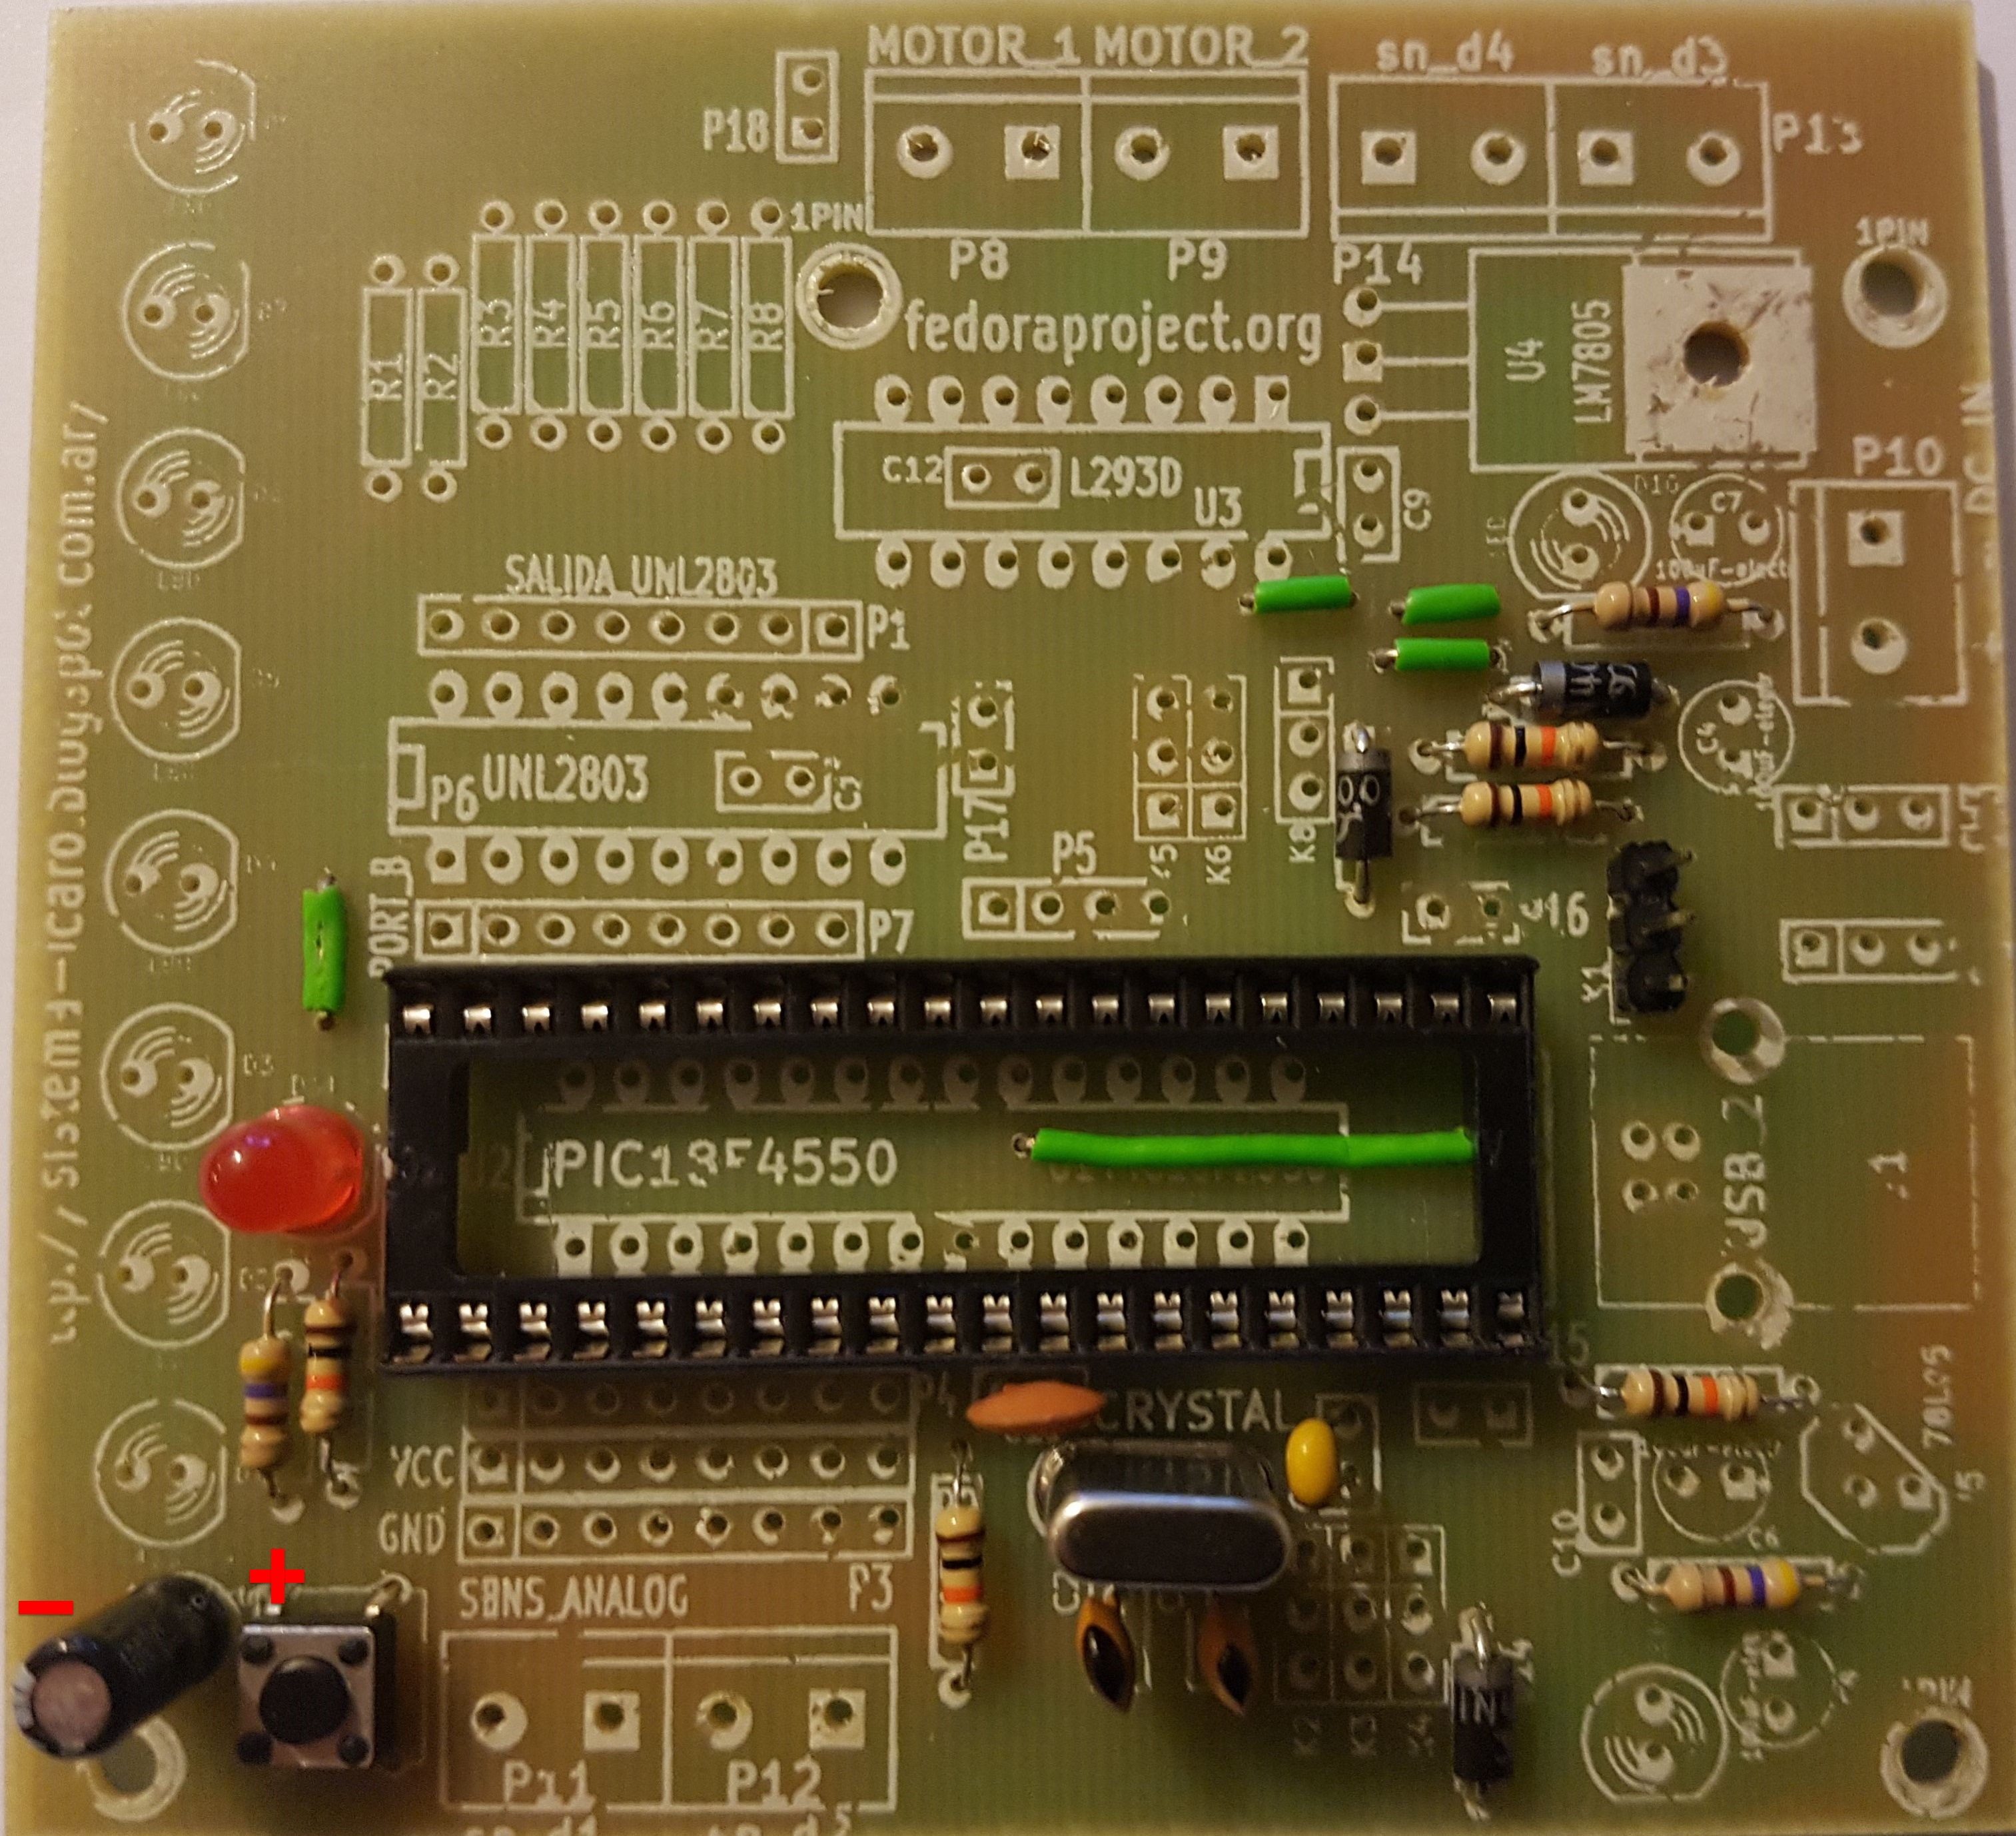
\includegraphics[width=0.8\linewidth]{Modulo_2/M2_9}
	\caption{Módulo 2 - Paso 9}
	\label{fig:M2_9}
\end{figure}

\newpage

\section{Paso 10:}

Instalar puerto USB. J1

\begin{figure}[h]
	\centering
	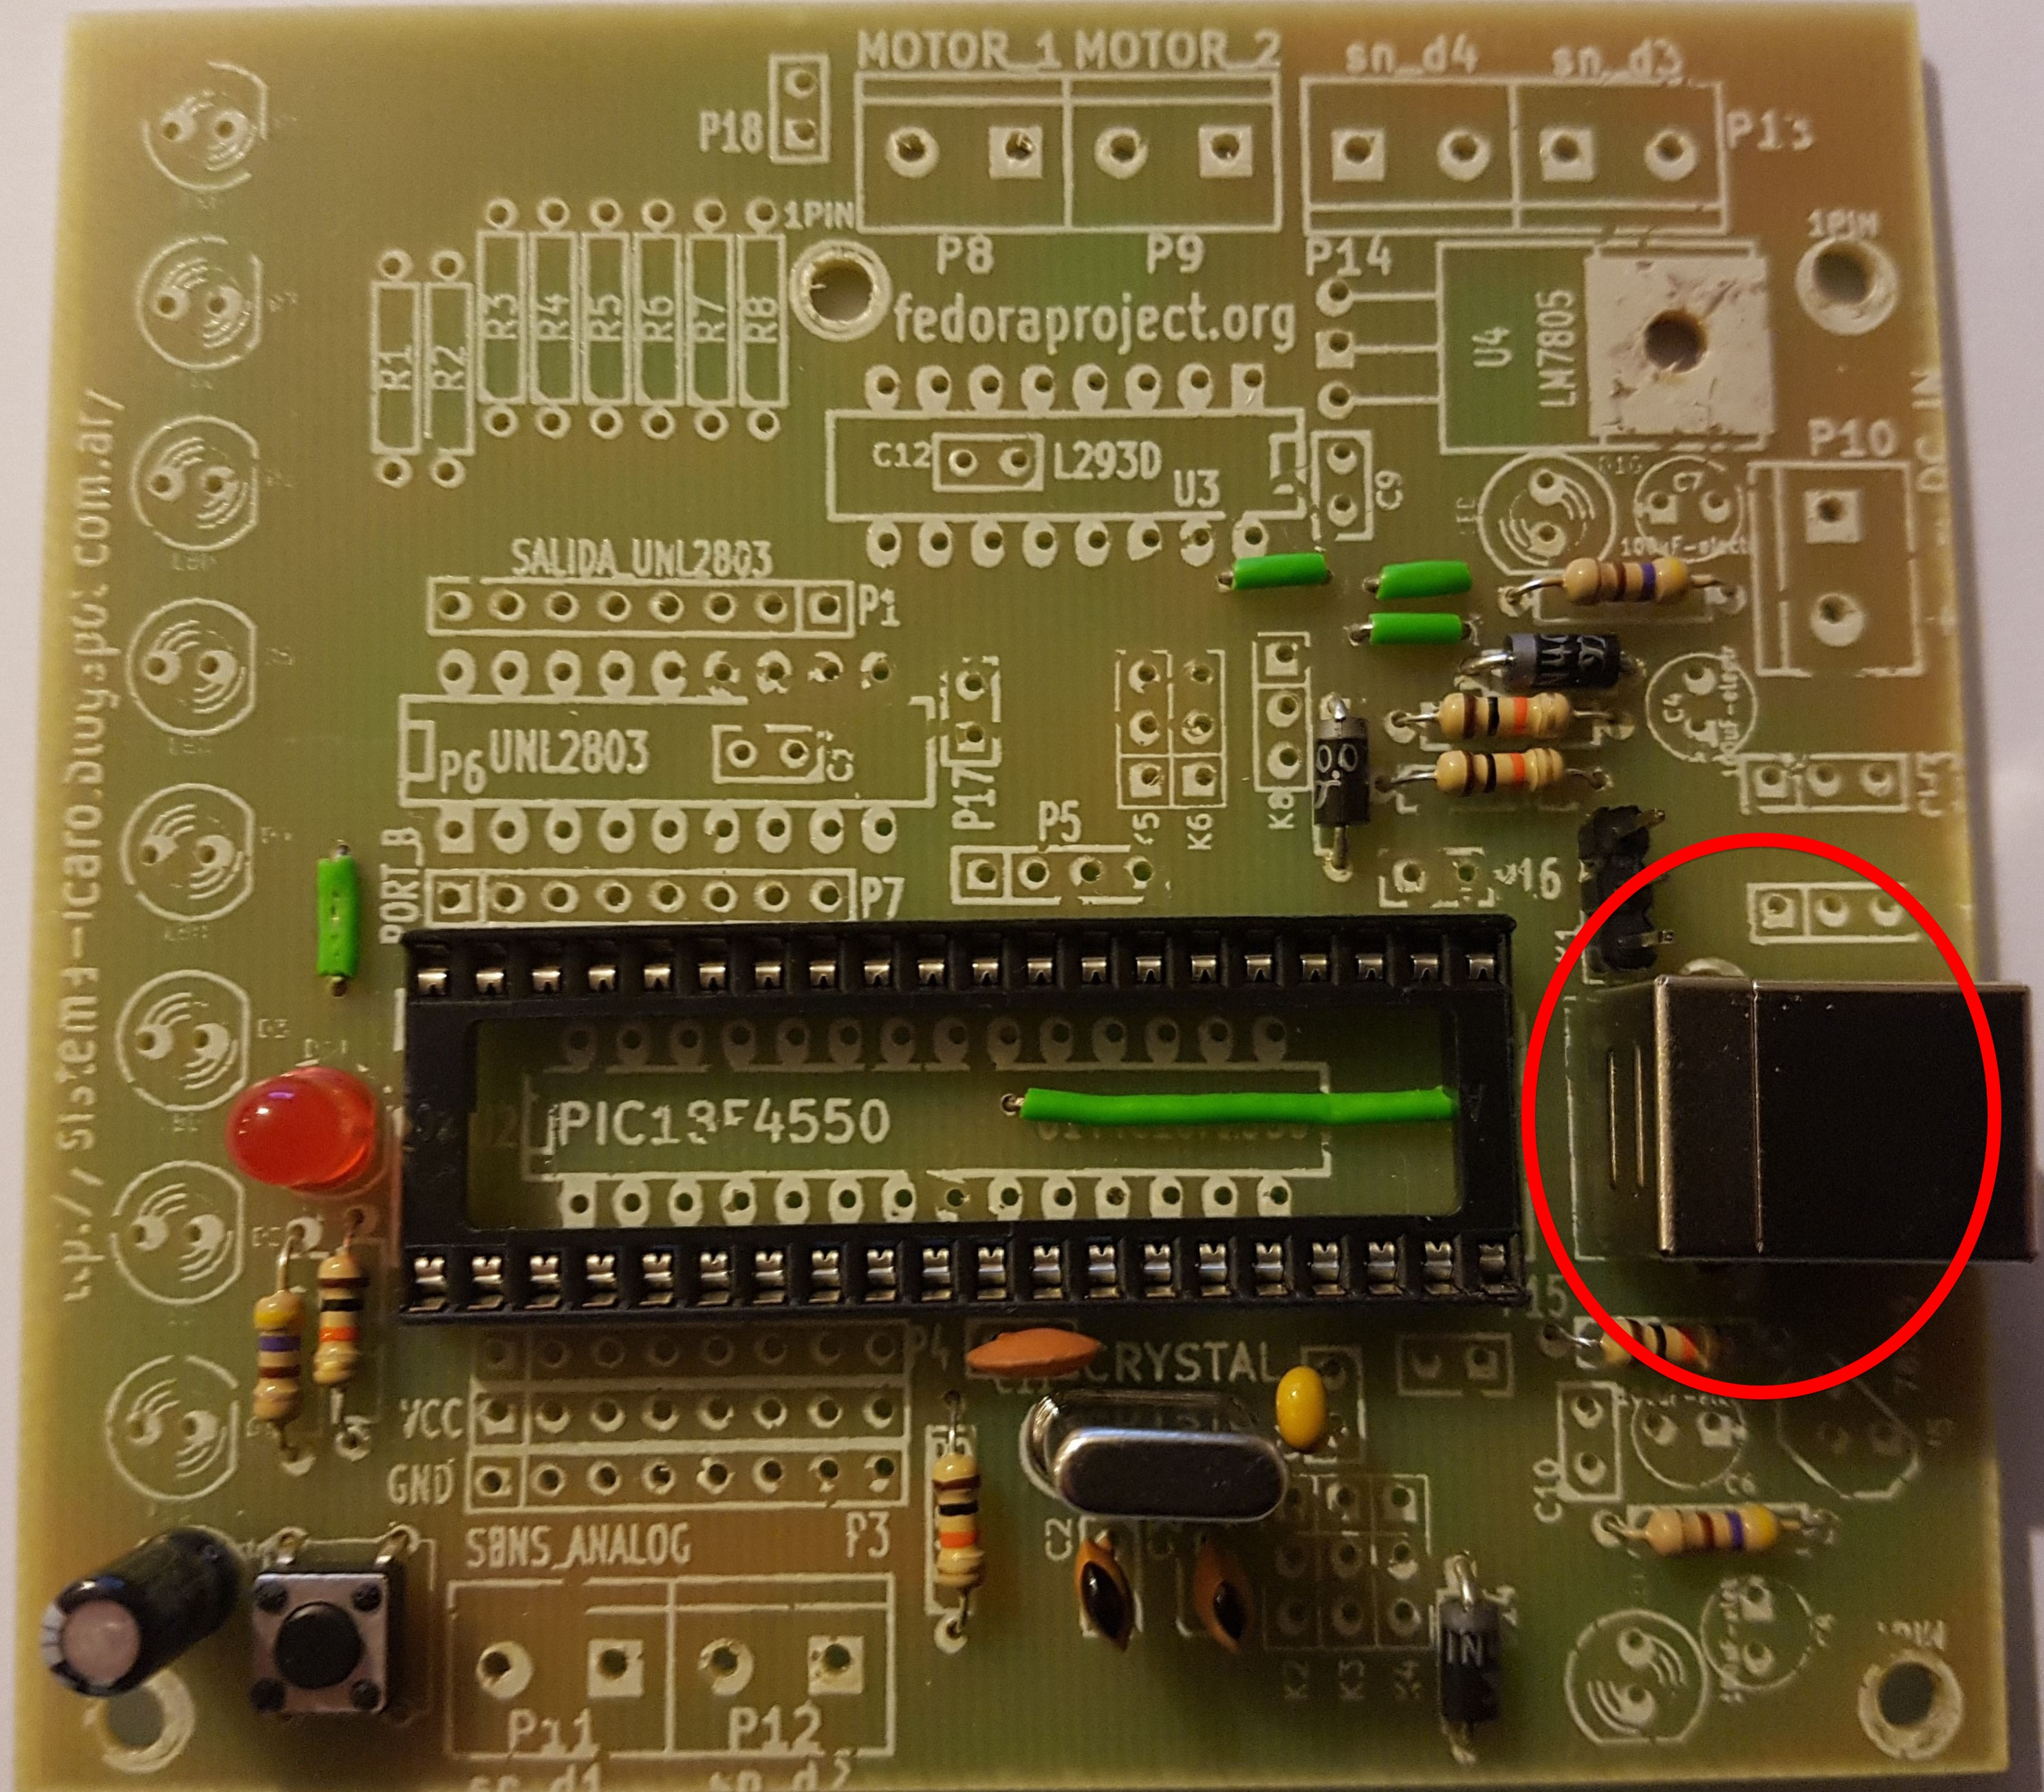
\includegraphics[width=0.8\linewidth]{Modulo_2/M2_10}
	\caption{Módulo 2 - Paso 10}
	\label{fig:M2_10}
\end{figure}

\newpage

\section{Paso 11:}

Instalar interruptor. SW1 y SW3. Opcionalmente se pueden usar pines machos

\begin{figure}[h]
	\centering
	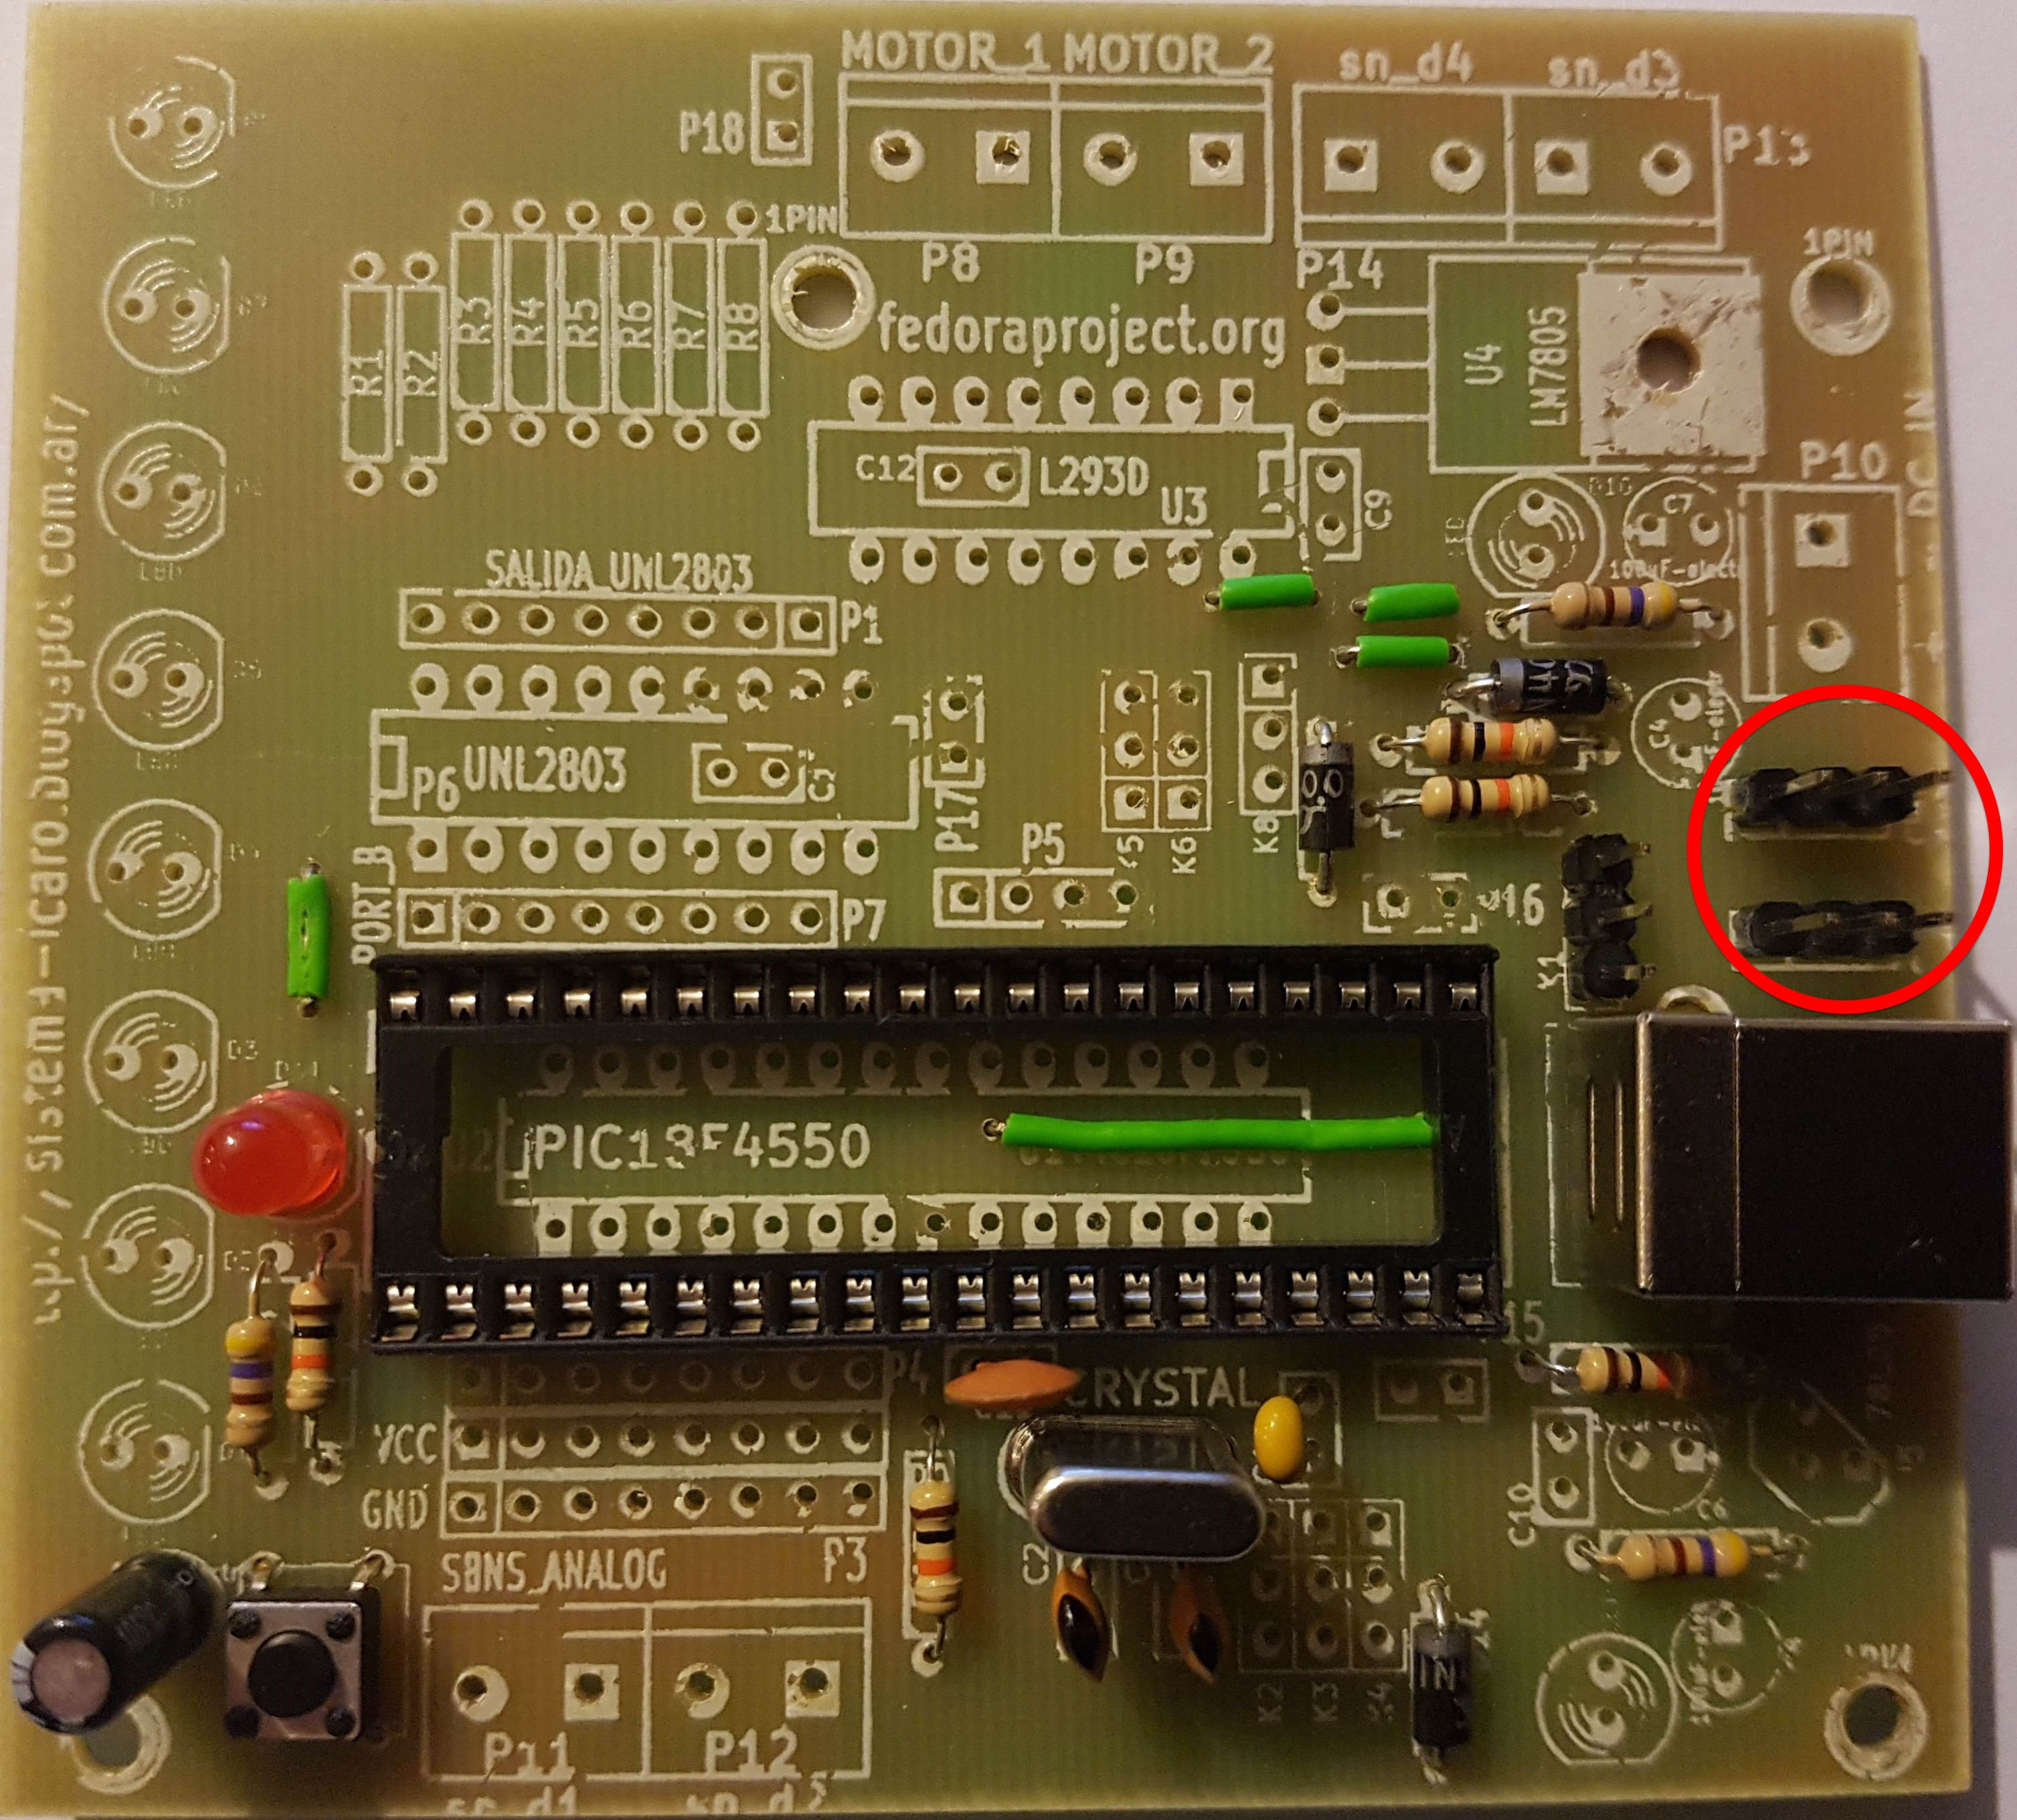
\includegraphics[width=0.8\linewidth]{Modulo_2/M2_11}
	\caption{Módulo 2 - Paso 11}
	\label{fig:M2_11}
\end{figure}

\newpage

\section{Paso 12:}

Instalar jumper en pines del lado del puerto USB en el selector K1

\begin{figure}[h]
	\centering
	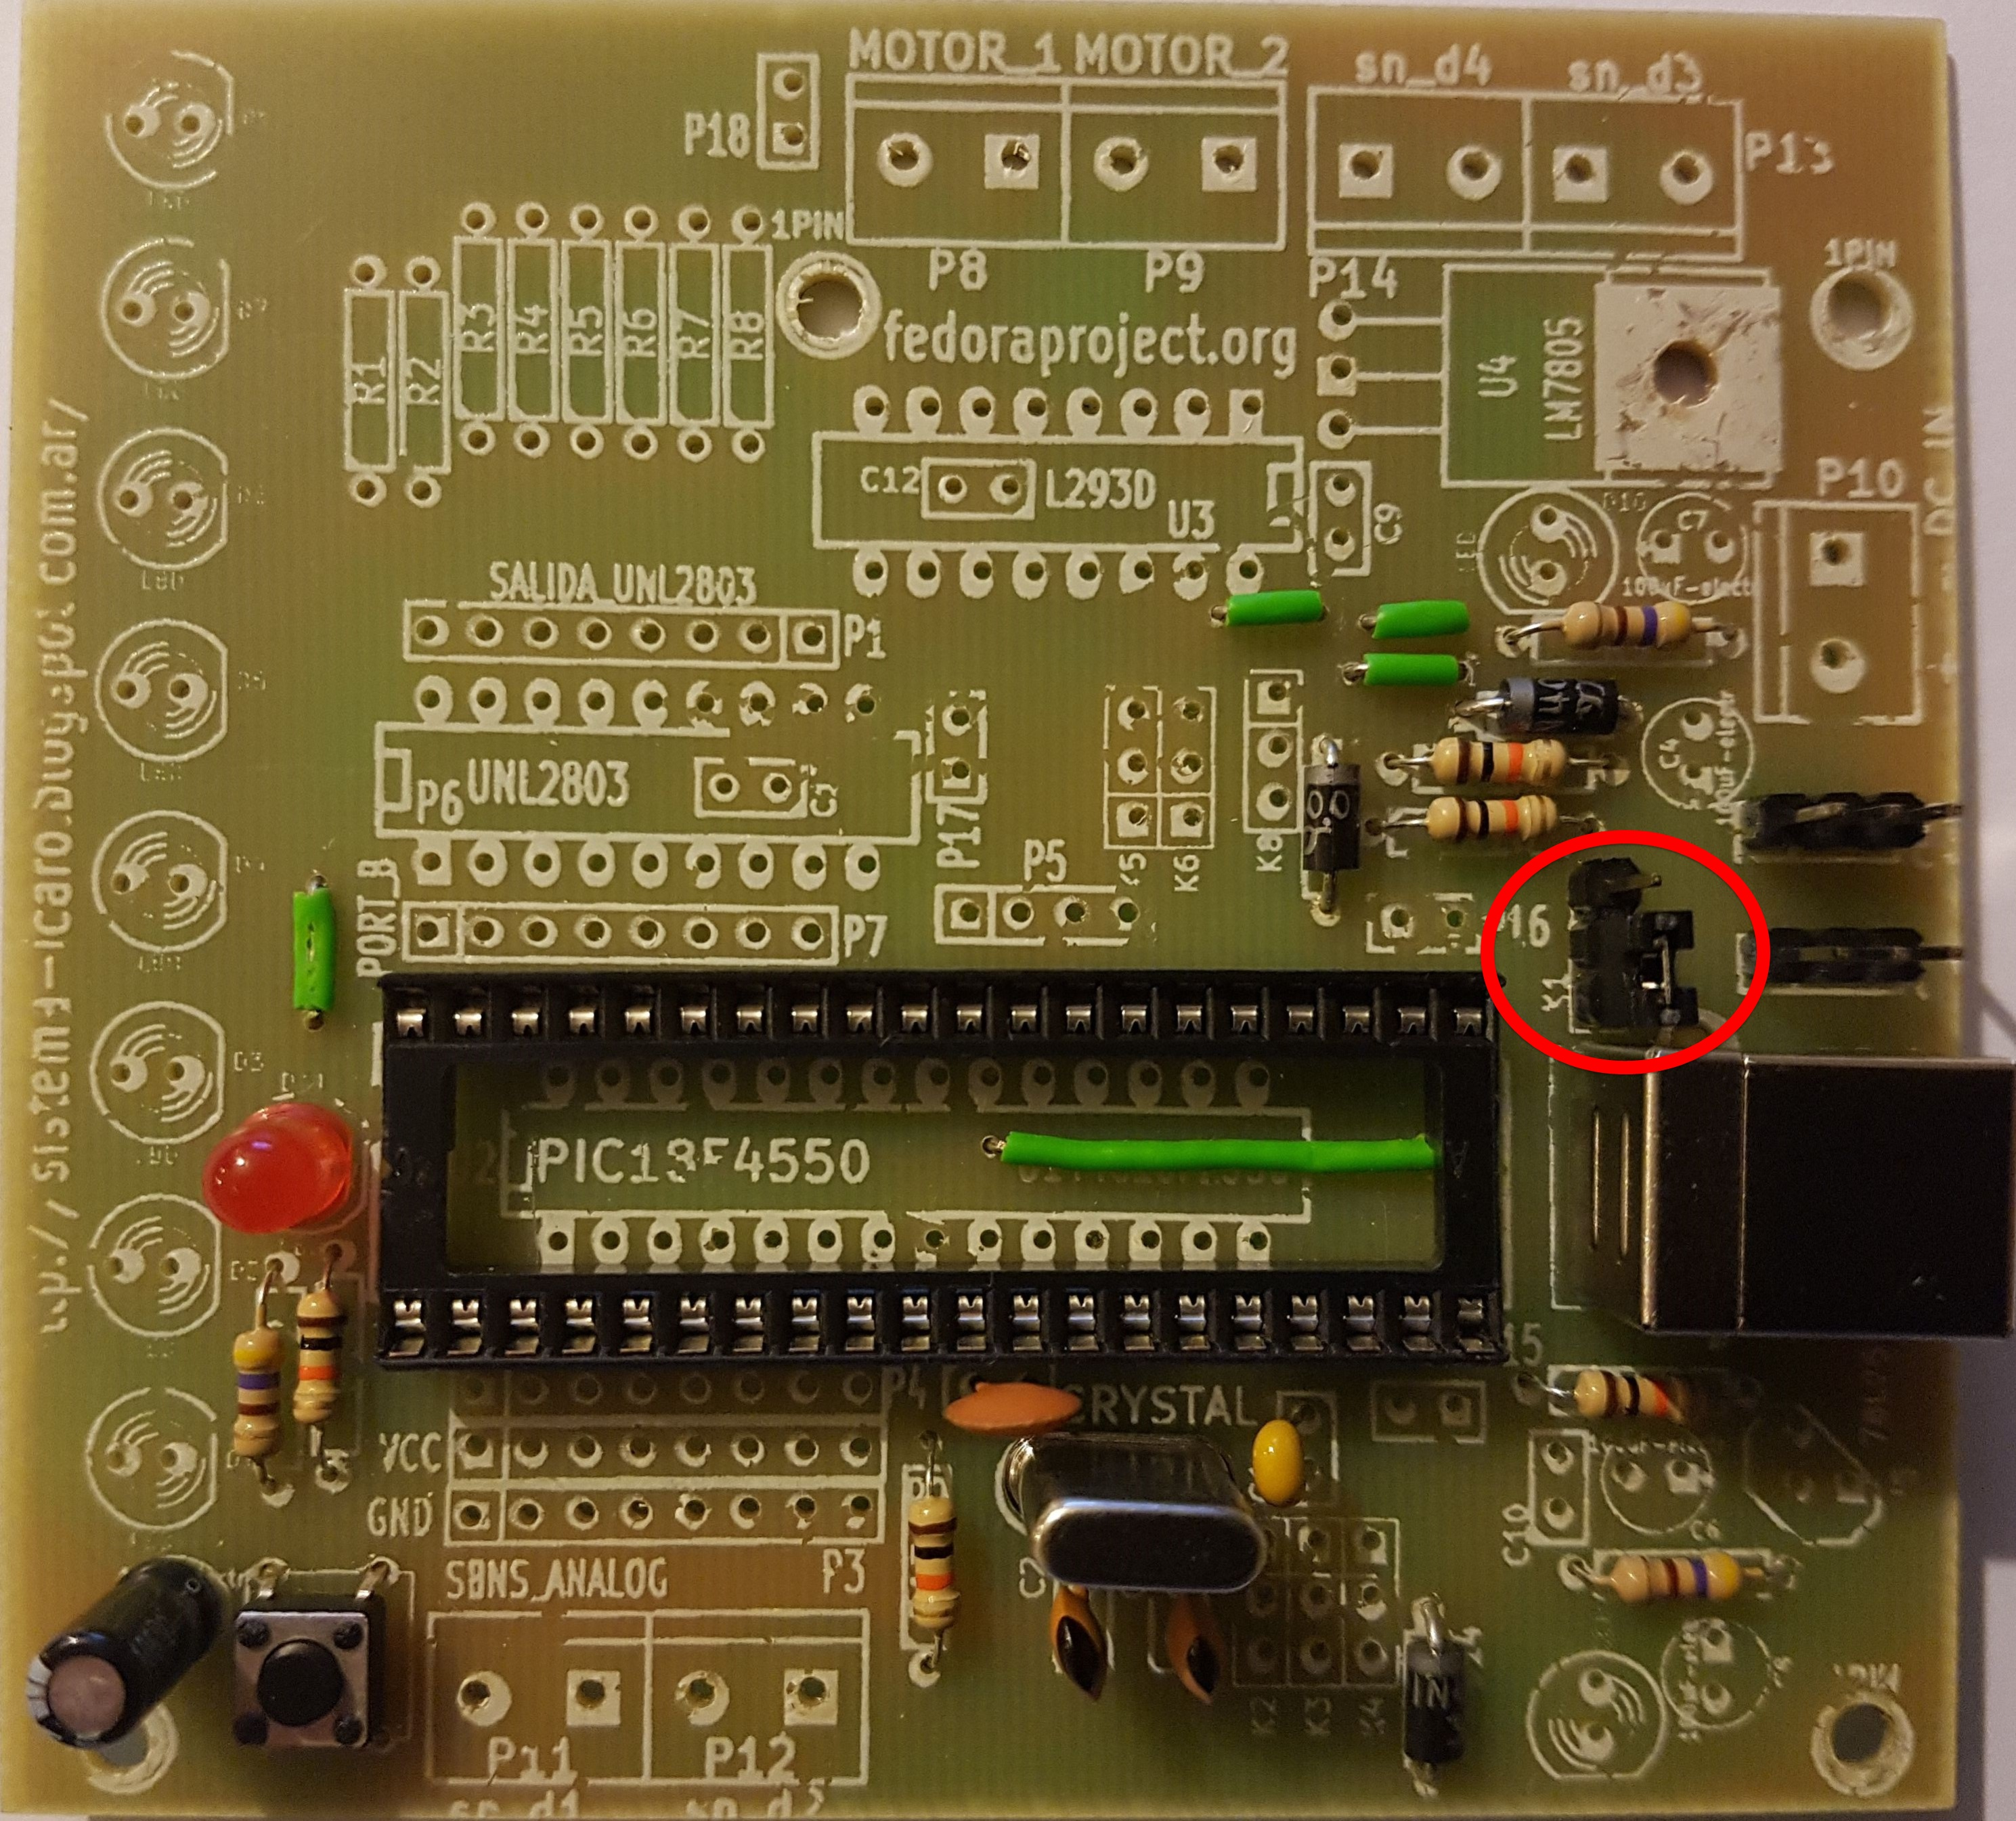
\includegraphics[width=0.8\linewidth]{Modulo_2/M2_12}
	\caption{Módulo 2 - Paso 12}
	\label{fig:M2_12}
\end{figure}

\newpage

\section{Paso 13:}

Instalar PIC 18F4550 en el Zócalo U2

\begin{figure}[h]
	\centering
	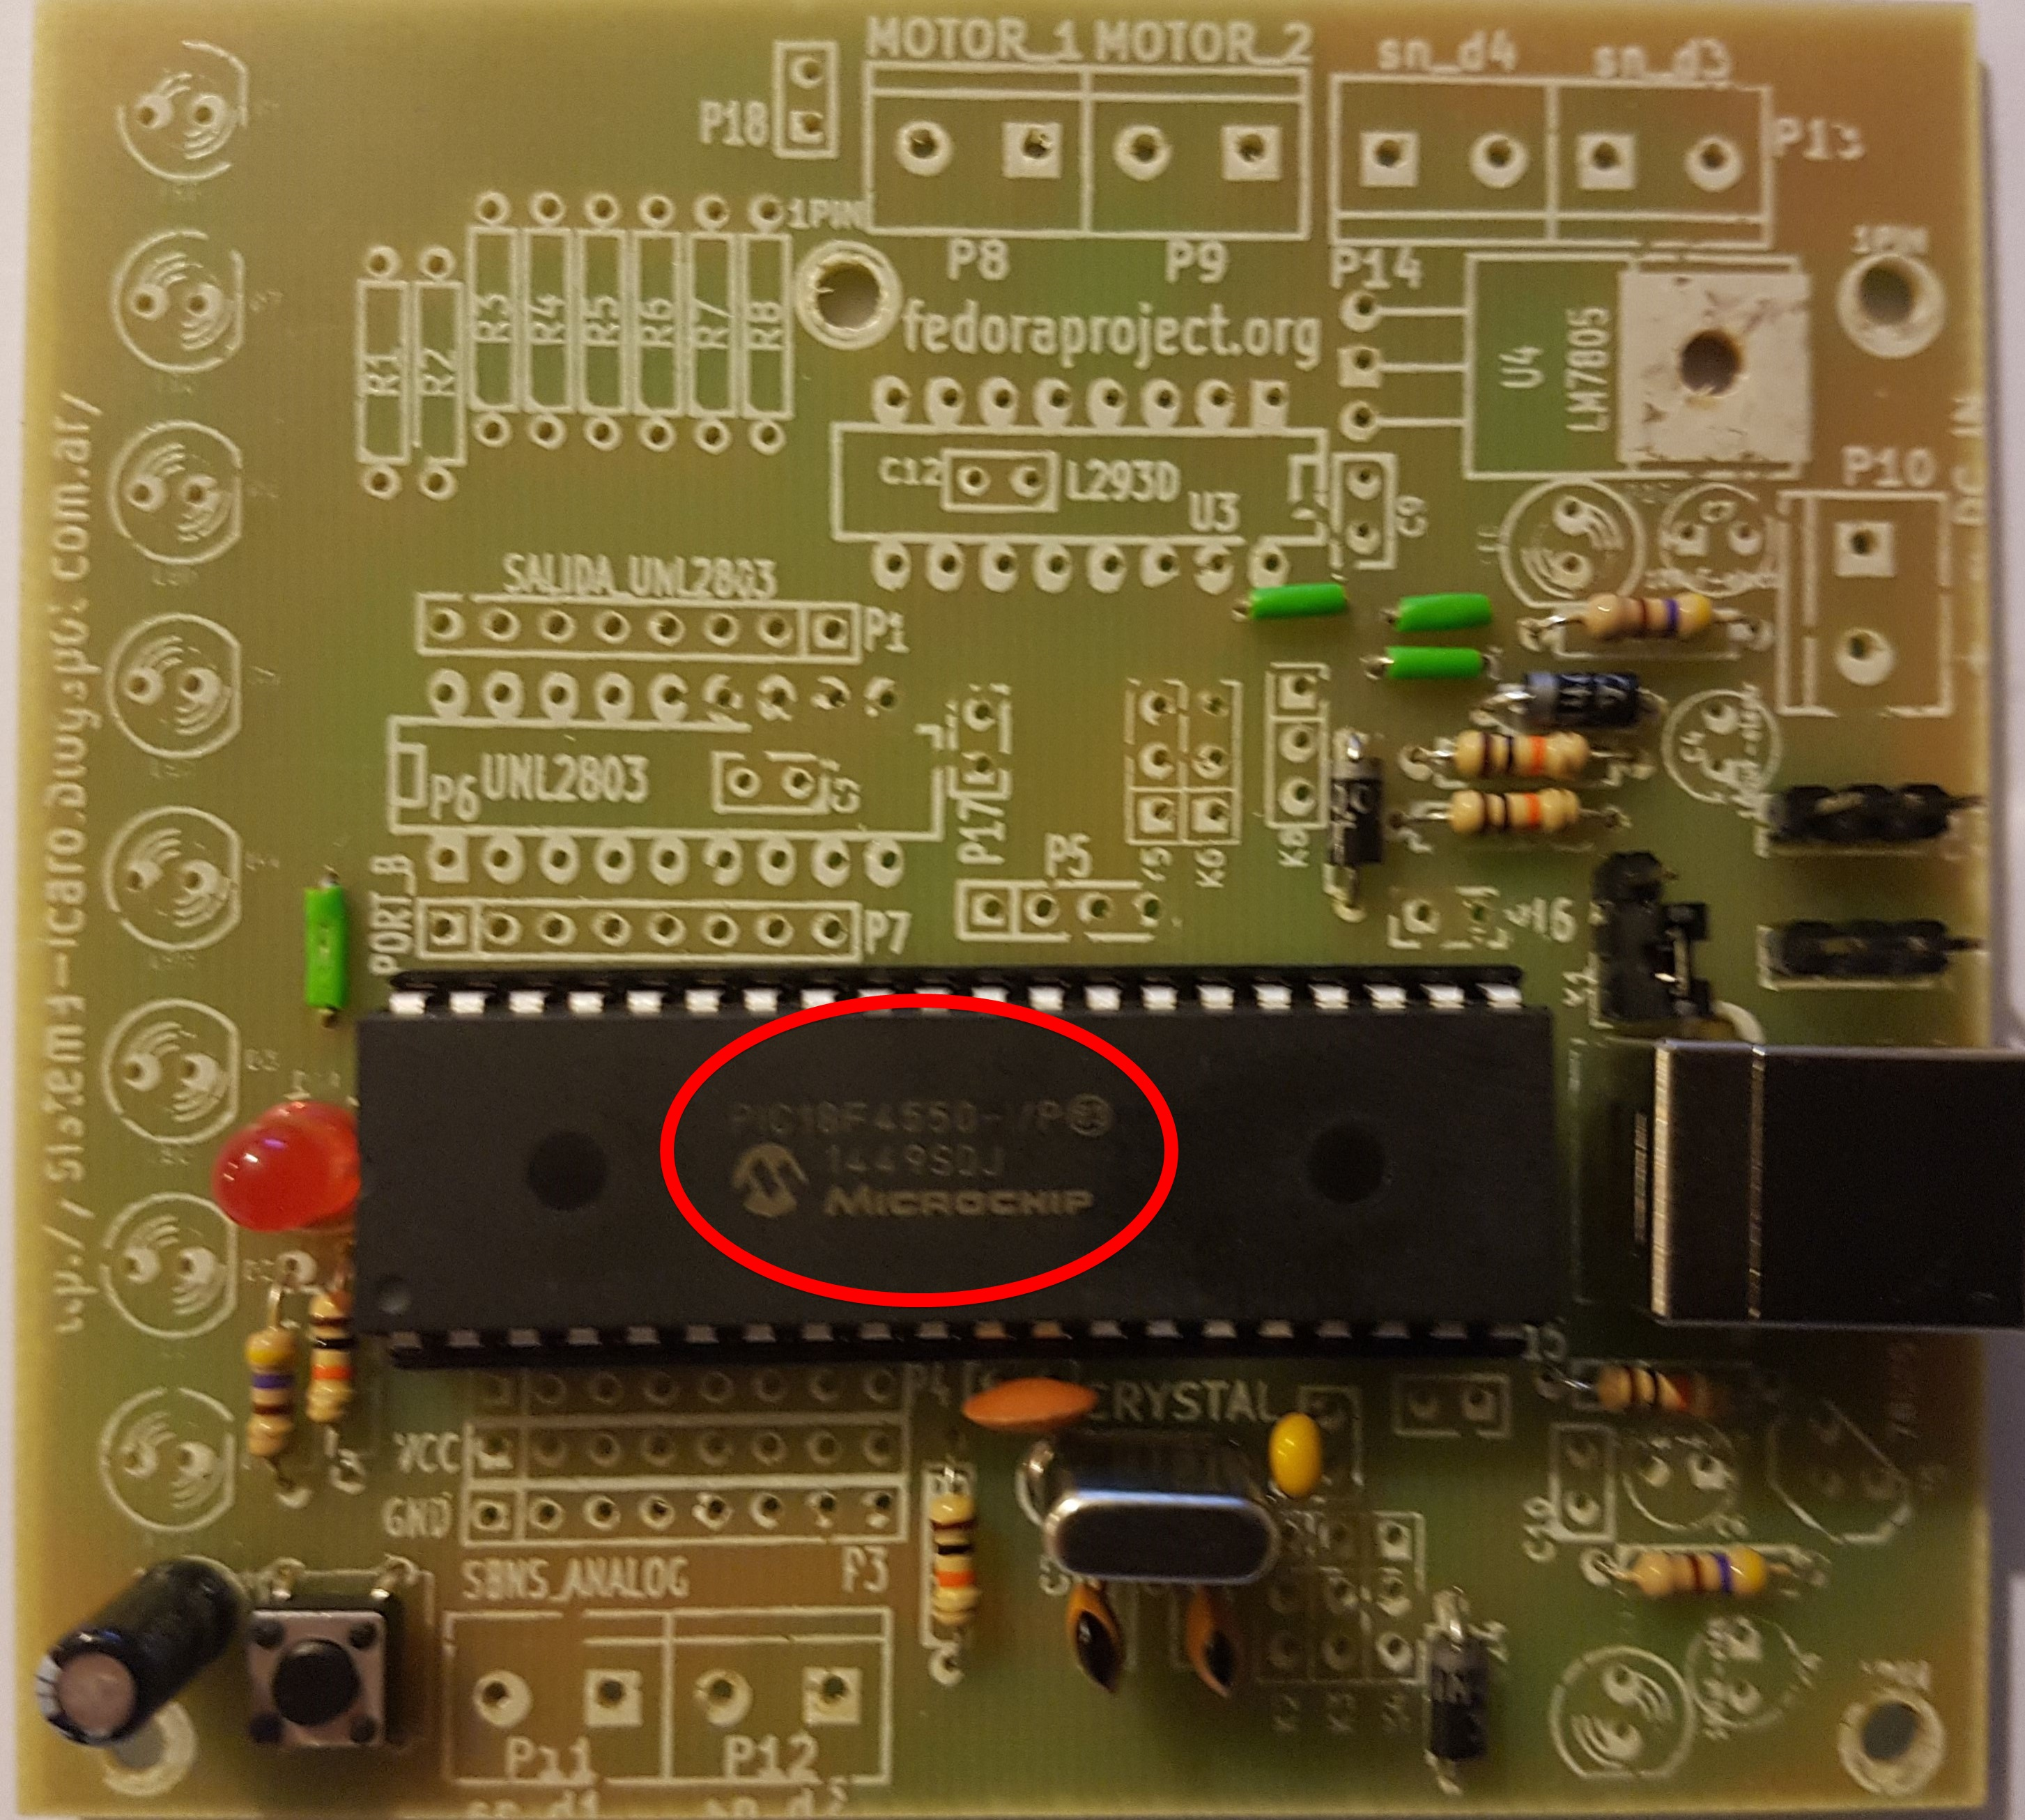
\includegraphics[width=0.8\linewidth]{Modulo_2/M2_13}
	\caption{Módulo 2 - Paso 13}
	\label{fig:M2_13}
\end{figure}

\newpage


NOTA: Las tiras de pines machos K5 y K6 podían instalarse en este momento para la comunicación con vía bluetooth HC-05. Para la comunicación solo se requieren los pines del lado del micro. Por comodidad se pueden instalar de una vez ambos puertos completos (los tres pines de cada puerto) y tener los pines para alimentación.

Comprobación
El puente al centro del micro debe dar +5VDC contra tierra.
El poner un micro con un script debe encender el led rojo D11

Nota: D11 no se enciende si el micro solo tiene el bootloader. Se puede cargar un programa en blanco de icaro bloques para probar que la placa levanta el micro. 



\chapter{Módulo 3: Leds y sensores digitales}

Si tiene instalado el microcontrolador, removerlo del zócalo

\section{Paso 1:}

Instalar resistencias faltantes. R1 a R8

\begin{figure}[h]
	\centering
	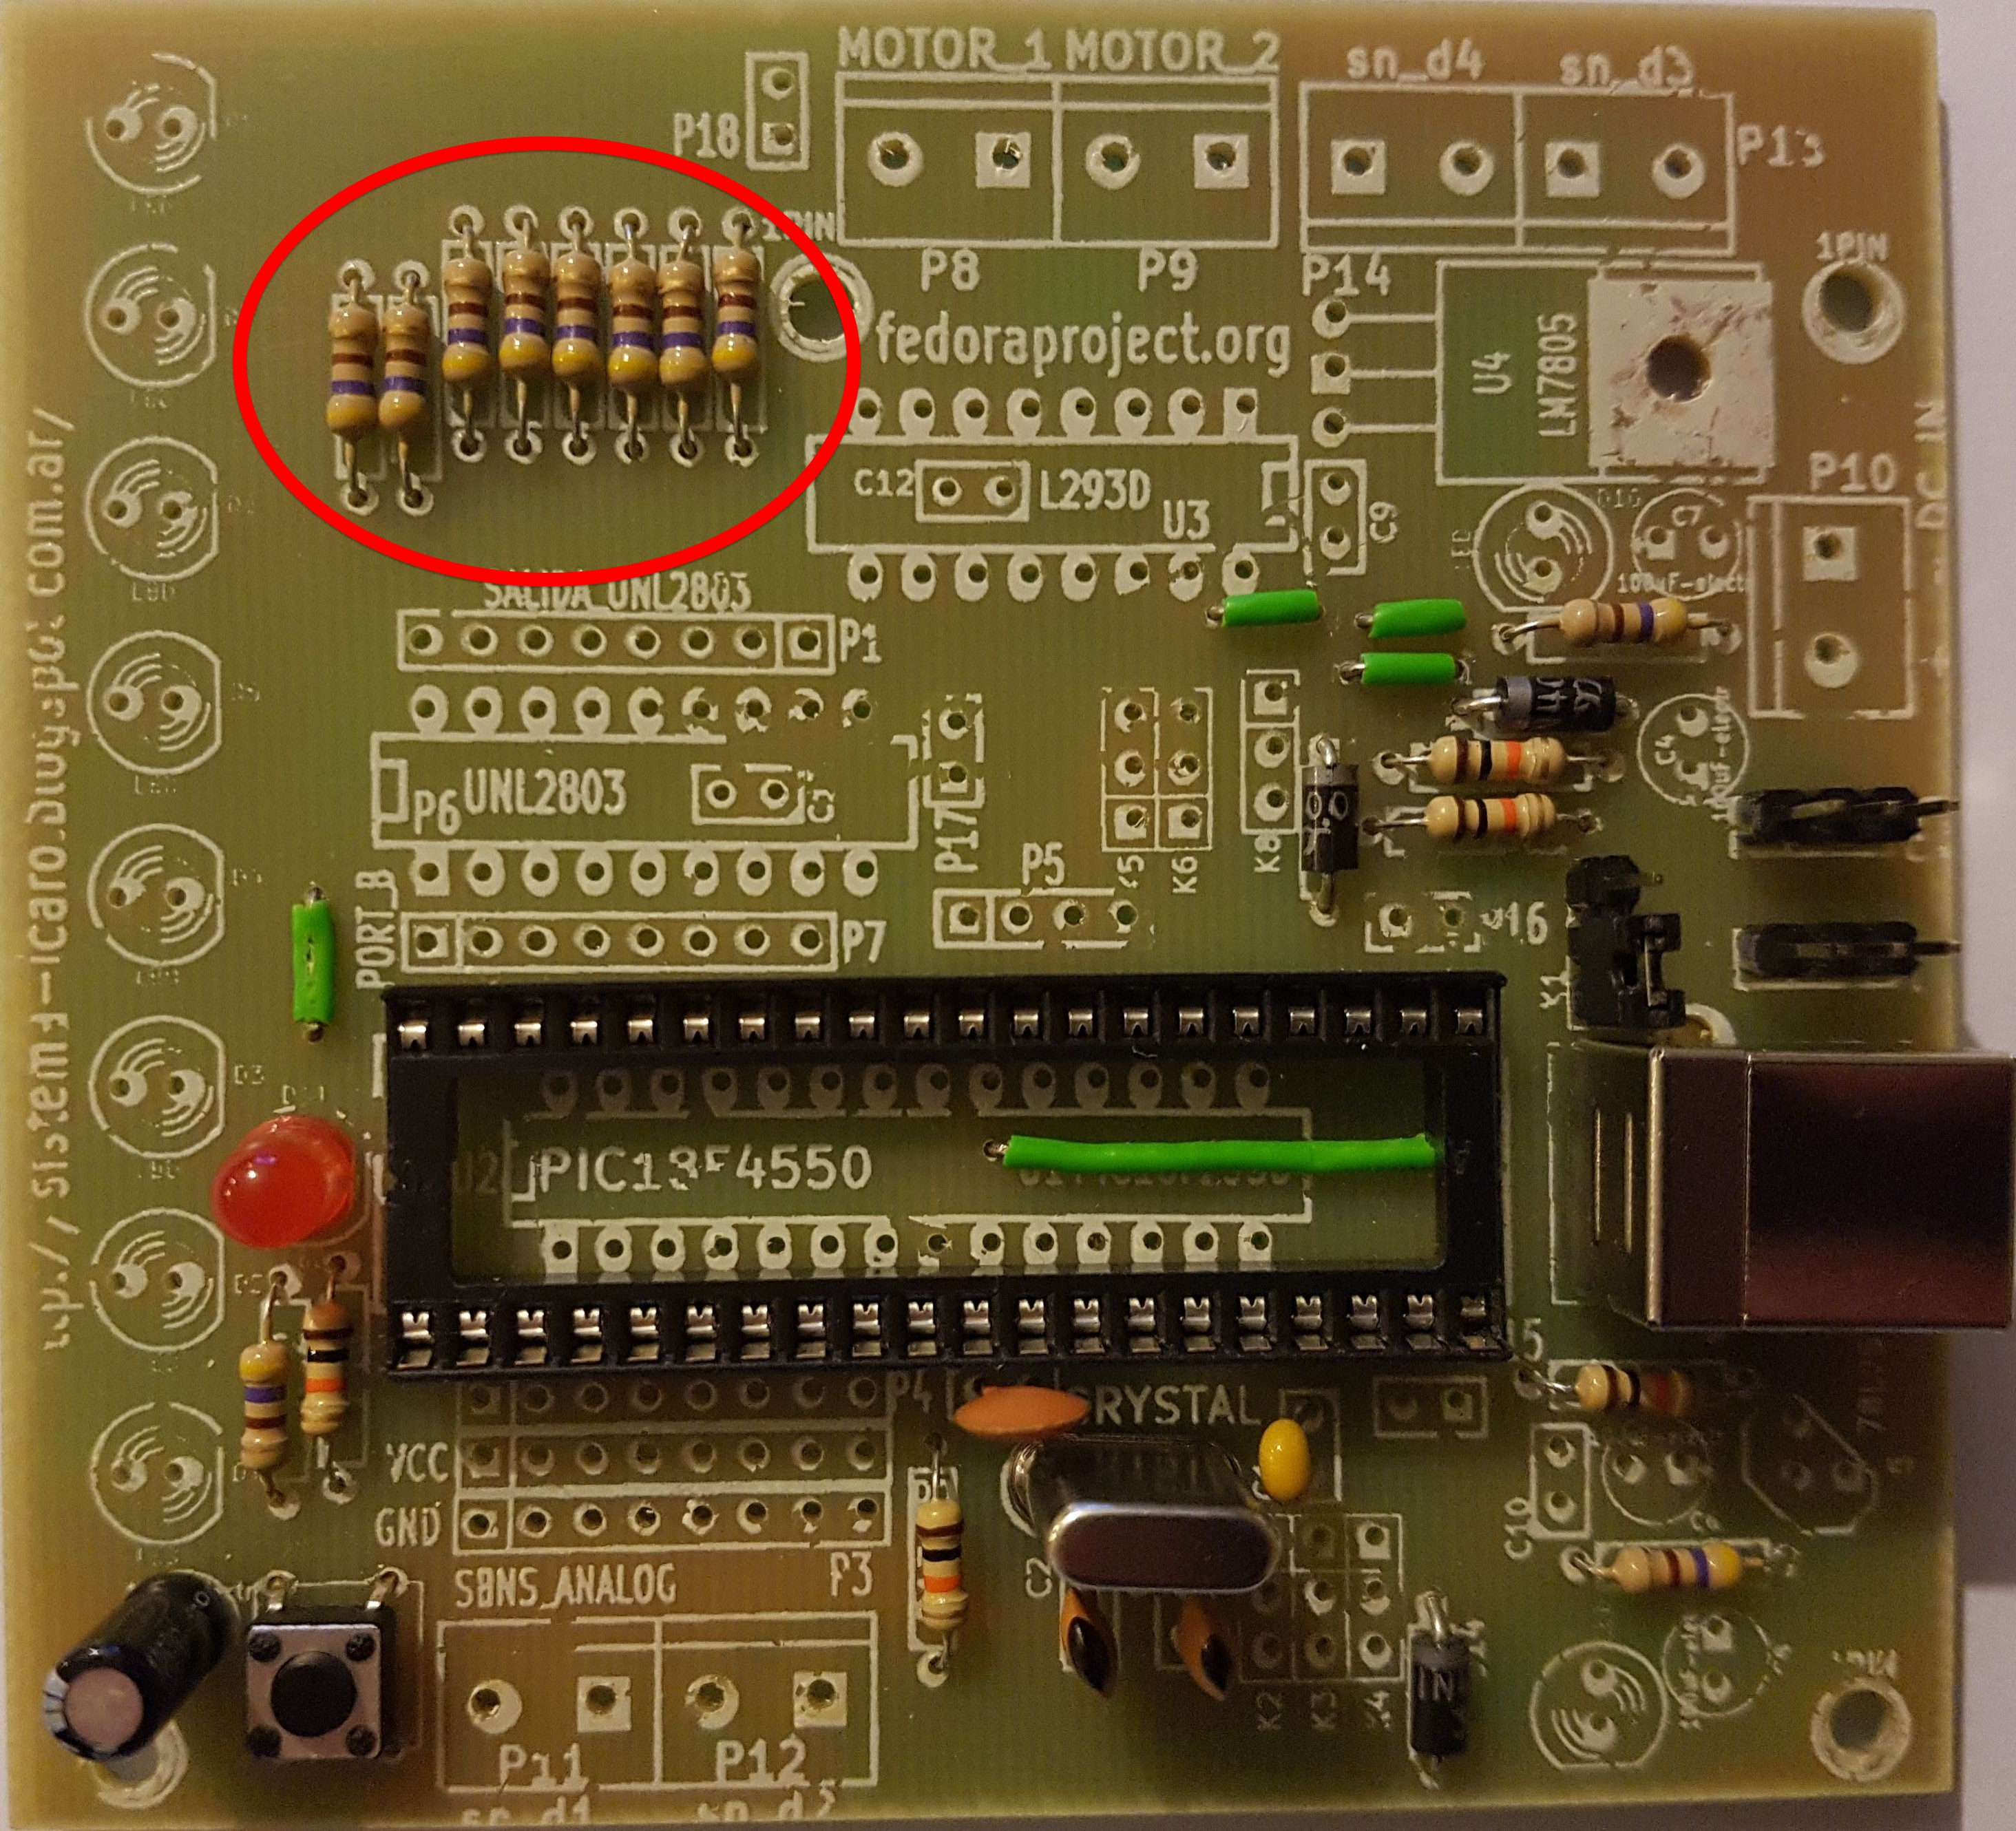
\includegraphics[width=0.8\linewidth]{Modulo_3/M3_1}
	\caption{Módulo 3 - Paso 1}
	\label{fig:M3_1}
\end{figure}

\newpage

\section{Paso 2:}

Instalar capacitor cerámico 0.1uF C13

\begin{figure}[h]
	\centering
	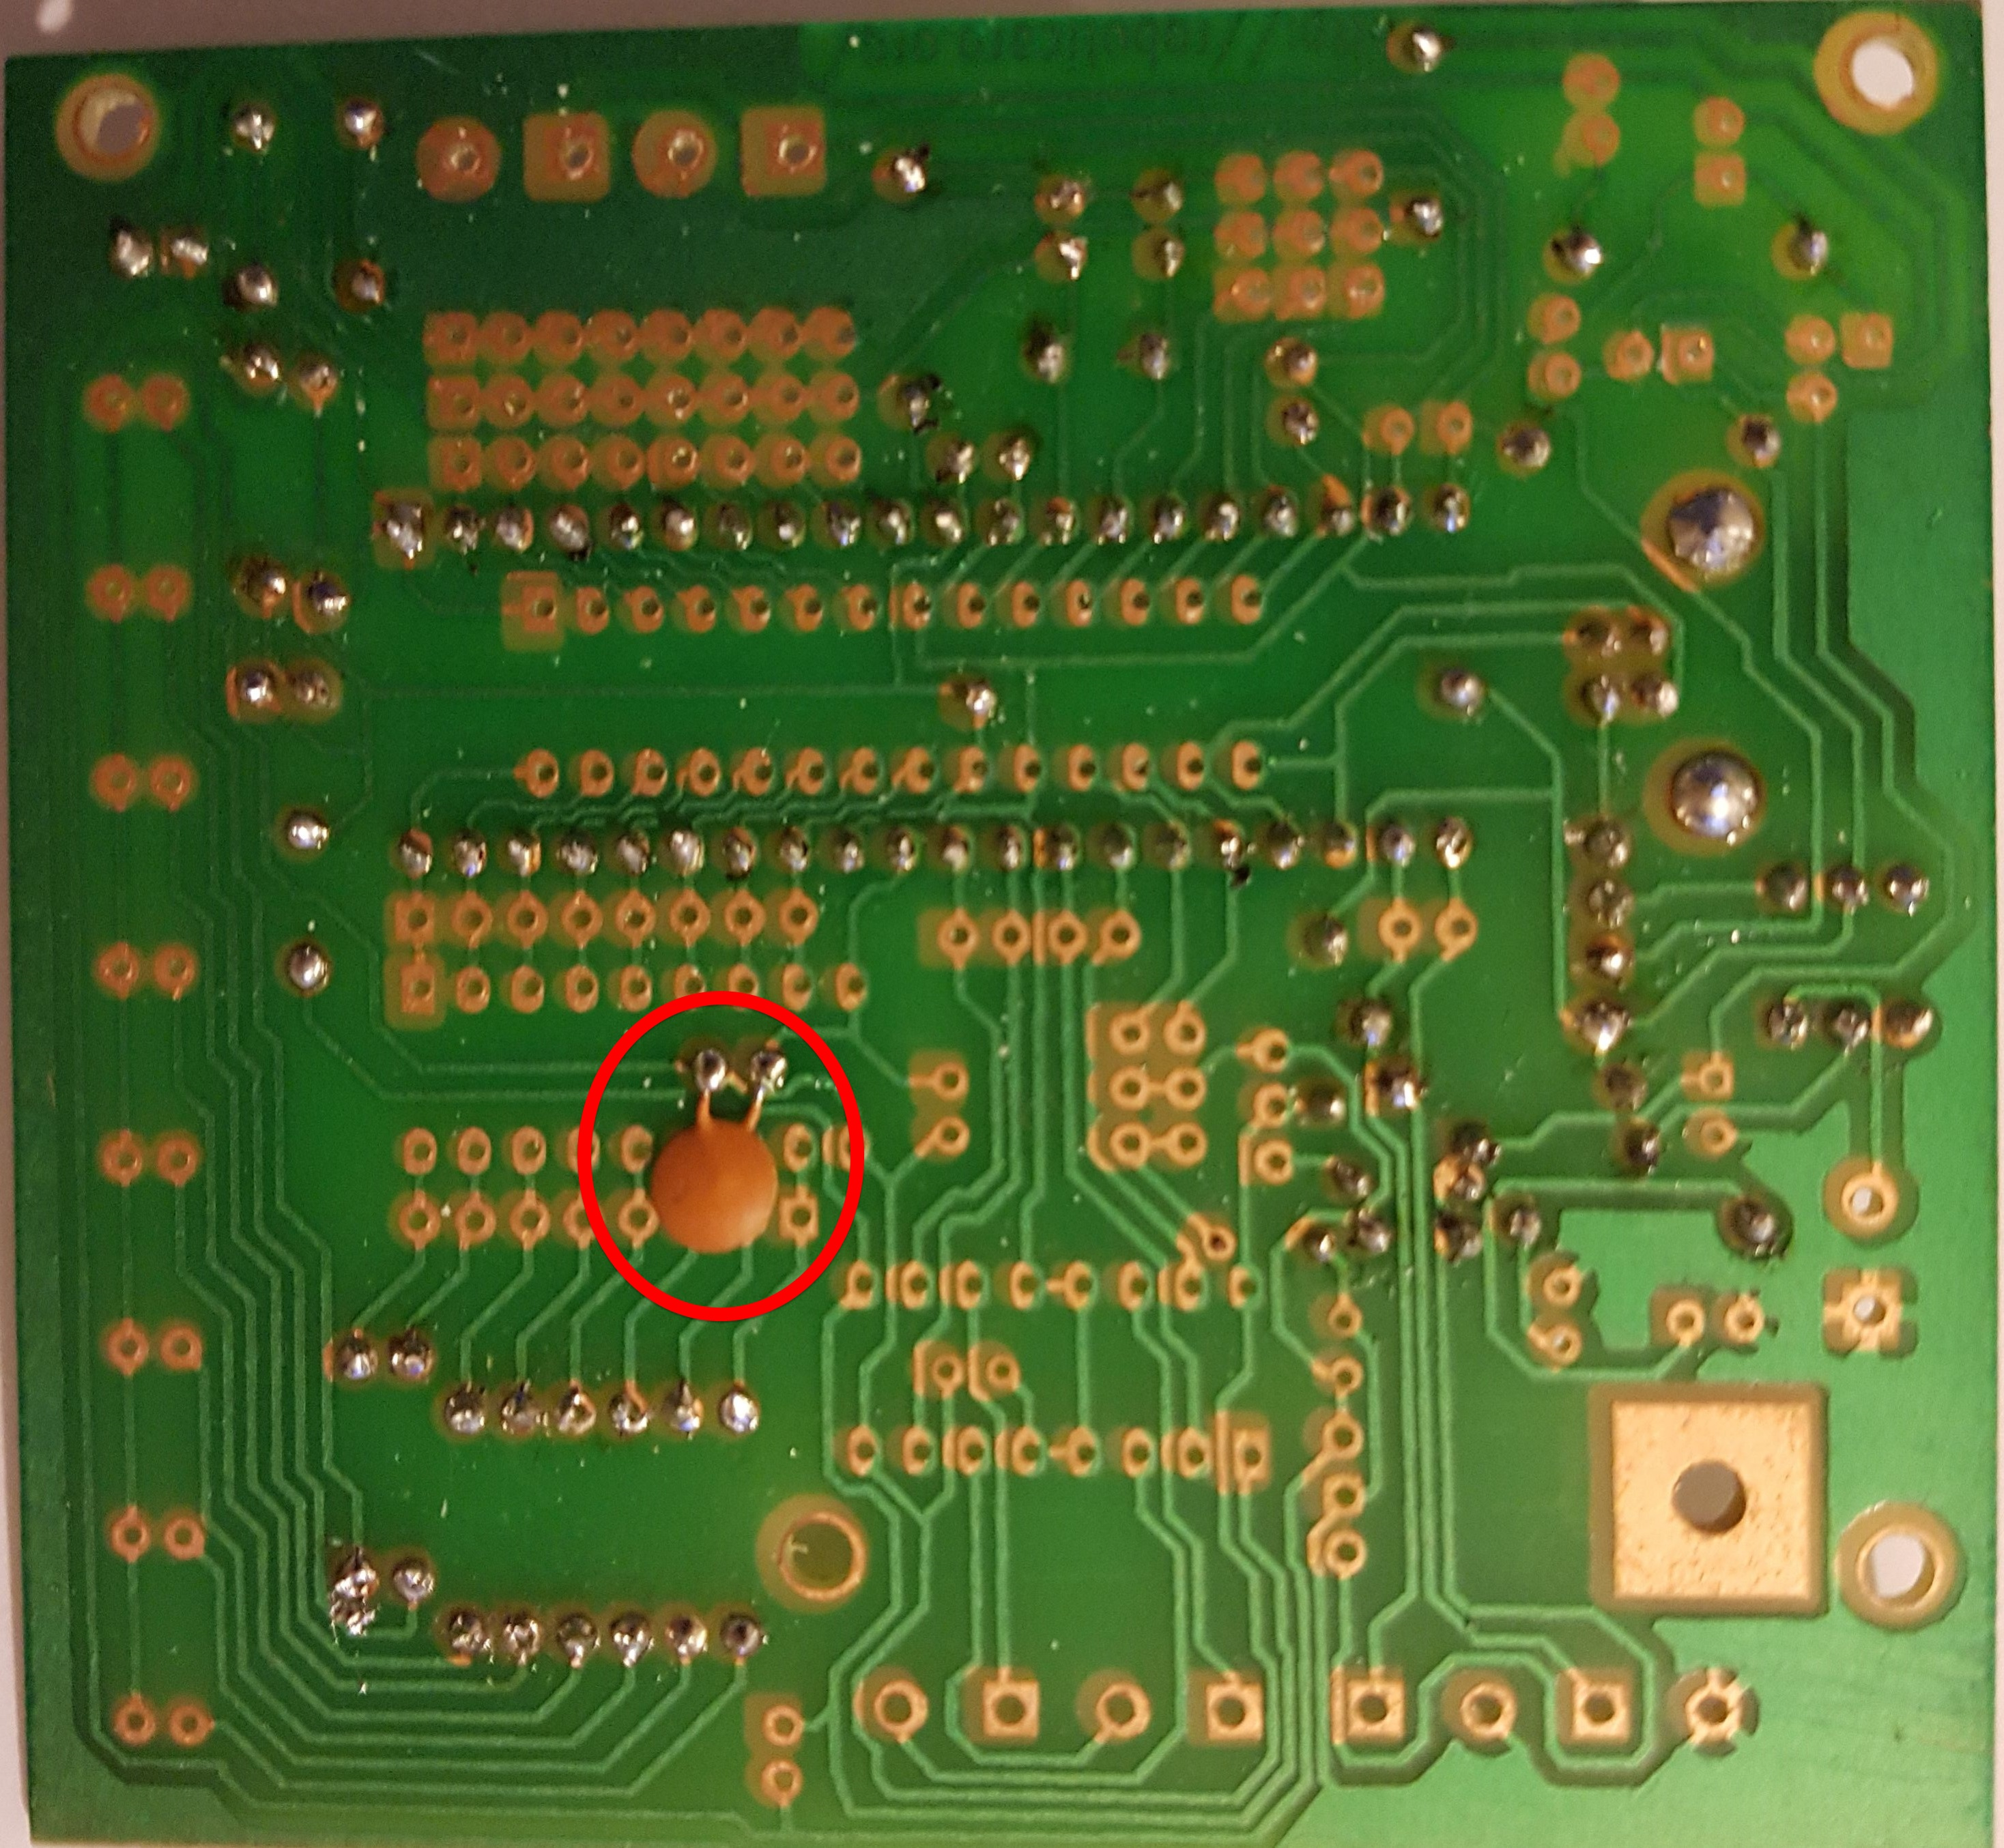
\includegraphics[width=0.8\linewidth]{Modulo_3/M3_2}
	\caption{Módulo 3 - Paso 2}
	\label{fig:M3_2}
\end{figure}

\newpage

\section{Paso 3:}

Instalar zócalo de 18 patas (9x2) P6 Tomar en cuenta alinear la muesca del diagrama de la placa con la muesca del zócalo.

\begin{figure}[h]
	\centering
	\includegraphics[width=0.8\linewidth]{Modulo_3/M3_3}
	\caption{Módulo 3 - Paso 3}
	\label{fig:M3_3}
\end{figure}

\newpage

\section{Paso 4:}

Instalar pines hembras (Port B) P7

\begin{figure}[h]
	\centering
	\includegraphics[width=0.8\linewidth]{Modulo_3/M3_4}
	\caption{Módulo 3 - Paso 4}
	\label{fig:M3_4}
\end{figure}

\newpage
\section{Paso 5:}

Instalar pines hembras P1

\begin{figure}[h]
	\centering
	\includegraphics[width=0.8\linewidth]{Modulo_3/M3_5}
	\caption{Módulo 3 - Paso 5}
	\label{fig:M3_5}
\end{figure}

\newpage

\section{Paso 6:}

Instalar leds de la barra de indicación. D1 a D8. Se recomienda todos del mismo color.

\begin{figure}[h]
	\centering
	\includegraphics[width=0.8\linewidth]{Modulo_3/M3_6}
	\caption{Módulo 3 - Paso 6}
	\label{fig:M3_6}
\end{figure}

\newpage

\section{Paso 7:}

Instalar pines hembras P15 (Se puede usar como entrada de P11 y P12)

\begin{figure}[h]
	\centering
	\includegraphics[width=0.8\linewidth]{Modulo_3/M3_7}
	\caption{Módulo 3 - Paso 7}
	\label{fig:M3_7}
\end{figure}

\newpage

\section{Paso 8:}

Instalar pines hembras P16 (Se puede usar como entrada de P13 y P14)

\begin{figure}[h]
	\centering
	\includegraphics[width=0.8\linewidth]{Modulo_3/M3_8}
	\caption{Módulo 3 - Paso 8}
	\label{fig:M3_8}
\end{figure}

\newpage

\section{Paso 9:}

Instalar borneras de 2 posiciones P11 a P14

\begin{figure}[h]
	\centering
	\includegraphics[width=0.8\linewidth]{Modulo_3/M3_9}
	\caption{Módulo 3 - Paso 9}
	\label{fig:M3_9}
\end{figure}

\newpage

\section{Paso 10:}

Instalar UNL2803 en P6

\begin{figure}[h]
	\centering
	\includegraphics[width=0.8\linewidth]{Modulo_3/M3_10}
	\caption{Módulo 3 - Paso 1}
	\label{fig:M3_10}
\end{figure}

\newpage

Comprobación:
Instalar el microcontrolador si no está instalado.
Cargar un script de ejemplos de la sección de leds y ver si los leds se encienden.
Cargar un script de ejemplos de la sección de icaro testing llamado sensores digitales. Con un cable o alambre, hacer corto entre los polos de la bornera sn-d1 y ver si el led D8 se enciende. Luego hacer corto entre los polos de la bornera sn-d2 y ver si el led D7 se enciende. Luego hacer corto entre los polos de la bornera sn-d3 y ver si el led D6 se enciende. Finalmente hacer corto entre los polos de la bornera sn-d4 y ver si el led D5 se enciende. 



\chapter{Módulo 4: Preparación}

Si tiene instalado el microcontrolador y el UNL2803, removerlos de sus zócalo antes de proseguir.

\section{Paso 1:}

Instalar pines hembras P4 (Pines para señal de entrada analógica)

\begin{figure}[h]
	\centering
	\includegraphics[width=0.8\linewidth]{Modulo_4/M4_1}
	\caption{Módulo 4 - Paso 1}
	\label{fig:M4_1}
\end{figure}

\newpage

\section{Paso 2:}

Instalar tira de pines hembras VCC. P2

\begin{figure}[h]
	\centering
	\includegraphics[width=0.8\linewidth]{Modulo_4/M4_2}
	\caption{Módulo 4 - Paso 2}
	\label{fig:M4_2}
\end{figure}

\newpage

\section{Paso 3:}

Instalar tira de pines hembras GND. P3

\begin{figure}[h]
	\centering
	\includegraphics[width=0.8\linewidth]{Modulo_4/M4_3}
	\caption{Módulo 4 - Paso 3}
	\label{fig:M4_3}
\end{figure}

\newpage

\section{Paso 4:}

Instalar tira de pines machos de servos. K2 a K6

\begin{figure}[h]
	\centering
	\includegraphics[width=0.8\linewidth]{Modulo_4/M4_4}
	\caption{Módulo 4 - Paso 4}
	\label{fig:M4_4}
\end{figure}

\newpage

Comprobación:
Cargar un script de ejemplos de la sección de icaro testing, sensors analogicos. Debe encenderse el led D8 y luego varios led aleatorios. Luego el led D7 y luego varios led aleatorios. Asi con cada uno de los leds. Los leds aleatorios son el valor de ruido que recibe el sensor analogico.



\chapter{Módulo 5: Motores de Corriente Continua}

\section{Paso 1:}

Instalar capacitor cerámico 0.1uF C12

\begin{figure}[h]
	\centering
	\includegraphics[width=0.8\linewidth]{Modulo_5/M5_1}
	\caption{Módulo 5 - Paso 1}
	\label{fig:M5_1}
\end{figure}

\newpage

\section{Paso 2:}

Instalar zócalo de 16 patas (2x8) U3 Tomar en cuenta alinear la muesca del diagrama de la placa con la muesca del zócalo.

\begin{figure}[h]
	\centering
	\includegraphics[width=0.8\linewidth]{Modulo_5/M5_2}
	\caption{Módulo 5 - Paso 2}
	\label{fig:M5_2}
\end{figure}

\newpage

\section{Paso 3:}

Instalar pines hembras P5 (Estos pines pueden usarse para tomar la señal que va al puente H)

\begin{figure}[h]
	\centering
	\includegraphics[width=0.8\linewidth]{Modulo_5/M5_3}
	\caption{Módulo 5 - Paso 3}
	\label{fig:M5_3}
\end{figure}

\newpage

\section{Paso 4:}

Instalar borneras de dos posiciones de motores. P8 y P9

\begin{figure}[h]
	\centering
	\includegraphics[width=0.8\linewidth]{Modulo_5/M5_4}
	\caption{Módulo 5 - Paso 4}
	\label{fig:M5_4}
\end{figure}

\newpage

\section{Paso 5:}

Instalar puente H L293D en U3

\begin{figure}[h]
	\centering
	\includegraphics[width=0.8\linewidth]{Modulo_5/M5_5}
	\caption{Módulo 5 - Paso 5}
	\label{fig:M5_5}
\end{figure}

\chapter{Módulo 6: Fuente de poder externa}

\section{Paso 1:}

Instalar regulador U4. LM7805. Es recomendable doblar las patitas antes de posicionarlo y soldarlo

\begin{figure}[h]
	\centering
	\includegraphics[width=0.8\linewidth]{Modulo_6/M6_1}
	\caption{Módulo 6 - Paso 1}
	\label{fig:M6_1}
\end{figure}

\newpage

\section{Paso 2:}

Instalar capacitor cerámico 0.1uF C9

\begin{figure}[h]
	\centering
	\includegraphics[width=0.8\linewidth]{Modulo_6/M6_2}
	\caption{Módulo 6 - Paso 2}
	\label{fig:M6_2}
\end{figure}

\newpage

\section{Paso 3:}

Instalar led de alimentación de motores. D10 (Se recomienda amarillo)

\begin{figure}[h]
	\centering
	\includegraphics[width=0.8\linewidth]{Modulo_6/M6_3}
	\caption{Módulo 6 - Paso 3}
	\label{fig:M6_3}
\end{figure}

\newpage

\section{Paso 4:}

Instalar capacitores electrolíticos 100uF C4 y C7

\begin{figure}[h]
	\centering
	\includegraphics[width=0.8\linewidth]{Modulo_6/M6_4}
	\caption{Módulo 6 - Paso 4}
	\label{fig:M6_4}
\end{figure}

\newpage

\section{Paso 5:}

Instalar bornera de dos posiciones para alimentación externa. P10

\begin{figure}[h]
	\centering
	\includegraphics[width=0.8\linewidth]{Modulo_6/M6_5}
	\caption{Módulo 6 - Paso 5}
	\label{fig:M6_5}
\end{figure}

\newpage

\section{Paso 6:}

Instalar capacitor cerámico 0.1uF C10

\begin{figure}[h]
	\centering
	\includegraphics[width=0.8\linewidth]{Modulo_6/M6_6}
	\caption{Módulo 6 - Paso 6}
	\label{fig:M6_6}
\end{figure}

\newpage

\section{Paso 7:}

Instalar capacitores electrolíticos 100uF C6 y C8

\begin{figure}[h]
	\centering
	\includegraphics[width=0.8\linewidth]{Modulo_6/M6_7}
	\caption{Módulo 6 - Paso 7}
	\label{fig:M6_7}
\end{figure}

\newpage

\section{Paso 8:}

Instalar regulador 78L05. U5. Se recomienda doblar la pata del centro hacia atrás en 45 grados y luego hacerle otro doblez para que quede paralela a las demás.


\begin{figure}[h]
	\centering
	\includegraphics[width=0.8\linewidth]{Modulo_6/M6_8}
	\caption{Módulo 6 - Paso 8}
	\label{fig:M6_8}
\end{figure}

\newpage

\section{Paso 9:}

Instalar led de alimentación de la placa. D13 Se recomienda color verde.

\begin{figure}[h]
	\centering
	\includegraphics[width=0.8\linewidth]{Modulo_6/M6_9}
	\caption{Módulo 6 - Paso 9}
	\label{fig:M6_9}
\end{figure}

\newpage

\section{Paso 10:}

Instalar tira de pines machos en el selector de voltaje. K8

\begin{figure}[h]
	\centering
	\includegraphics[width=0.8\linewidth]{Modulo_6/M6_10}
	\caption{Módulo 6 - Paso 10}
	\label{fig:M6_10}
\end{figure}

\newpage

\section{Paso 11:}

Instalar jumper en K8 del lado del micro

\begin{figure}[h]
	\centering
	\includegraphics[width=0.8\linewidth]{Modulo_6/M6_11}
	\caption{Módulo 6 - Paso 11}
	\label{fig:M6_11}
\end{figure}

\newpage

\section{Paso 12:}

Instalar tira de pines hembras P17 (es una toma de corriente)

\begin{figure}[h]
	\centering
	\includegraphics[width=0.8\linewidth]{Modulo_6/M6_12}
	\caption{Módulo 6 - Paso 12}
	\label{fig:M6_12}
\end{figure}

\newpage

\section{Paso 13:}

Instalar tira de pines hembras P18 (sirve para saltar un dio de protección y asegurar tener 5VDC. Solo ocupar en casos extremos y estando seguro del porque lo hace.

\begin{figure}[h]
	\centering
	\includegraphics[width=0.8\linewidth]{Modulo_6/M6_13}
	\caption{Módulo 6 - Paso 13}
	\label{fig:M6_13}
\end{figure}

\chapter{Historia de Revisión}


\begin{tabular}{|c|c|p{8cm}|c|}
	\hline
	\textbf{Fecha} & \textbf{Versión} & \textbf{Descripción}                                                          & \textbf{Autor}  \\[0.5cm] \hline\hline
	2016-10-23   &    Release 0     & Versión Inicial.                                                              & Mateo Carabajal \\[0.5cm] \hline
	2017-06-17   &   Release 1.0    & Se cambia la forma de explicar el armado, dividiendo el armado por 6 módulos. & Claudio Oliveda \\[0.5cm] \hline
\end{tabular} 






\end{document}
